
%            ███╗░░░███╗░█████╗░██████╗░██╗░░██╗
%            ████╗░████║██╔══██╗██╔══██╗██║░██╔╝
%            ██╔████╔██║███████║██████╔╝█████═╝░
%            ██║╚██╔╝██║██╔══██║██╔══██╗██╔═██╗░
%            ██║░╚═╝░██║██║░░██║██║░░██║██║░╚██╗
%            ╚═╝░░░░░╚═╝╚═╝░░╚═╝╚═╝░░╚═╝╚═╝░░╚═╝
 
%   ███╗░░██╗░██████╗░██╗░░░██╗██╗░░░██╗███████╗███╗░░██╗
%   ████╗░██║██╔════╝░██║░░░██║╚██╗░██╔╝██╔════╝████╗░██║
%   ██╔██╗██║██║░░██╗░██║░░░██║░╚████╔╝░█████╗░░██╔██╗██║
%   ██║╚████║██║░░╚██╗██║░░░██║░░╚██╔╝░░██╔══╝░░██║╚████║
%   ██║░╚███║╚██████╔╝╚██████╔╝░░░██║░░░███████╗██║░╚███║
%   ╚═╝░░╚══╝░╚═════╝░░╚═════╝░░░░╚═╝░░░╚══════╝╚═╝░░╚══╝



\documentclass{article}


%  ========== PREAMBLE ==========


% -= Packages =-

\usepackage[utf8]{vietnam}
\usepackage[top=1in,bottom=1in,left=1in,right=1in,paper=a4paper]{geometry}
\usepackage{graphicx,float}
\usepackage{hyperref}
\usepackage{tocloft}
\usepackage[immediate]{silence}
\WarningFilter[temp]{latex}{Command} % silence the warning
\usepackage{sectsty}
\DeactivateWarningFilters[temp] % So nothing unrelated gets silenced
\usepackage[most]{tcolorbox}
\usepackage{textcomp}
\usepackage{amsmath,amsfonts,amssymb,amsthm,mathtools,gensymb}
\usepackage{hyperref}
\usepackage{tikz}
\usepackage{titling}
\usepackage{lipsum}
\usepackage{mathtools}
\usepackage{enumitem}
\usepackage[utf8]{inputenc}
\usepackage[titletoc,title]{appendix}
\usepackage{xcolor}
\usepackage[twoside]{fancyhdr}
\usepackage[parfill]{parskip}
\usepackage{multicol}
\usepackage{pgfplots}
\pgfplotsset{compat=1.15}
\usepackage{mathrsfs}
\usetikzlibrary{arrows}
\usepackage{fontawesome5}
\usepackage{titlesec}
%\usepackage{mathpazo}

\usetikzlibrary{arrows.meta, decorations.pathreplacing,calc}

\makeatletter % disable the runtime redefinitions
\let\SS@makeulinesect\relax
\let\SS@makeulinepartchap\relax
\makeatother


% -= Settings =-

\pagestyle{fancy}
\allsectionsfont{\bfseries\sffamily}

\graphicspath{ {./images/} }

\hypersetup{
    colorlinks,
    citecolor=black,
    filecolor=black,
    linkcolor=purple,
    urlcolor=blue
}


\renewcommand{\baselinestretch}{1.5}
\newcommand{\qedblack}{$\hfill\blacksquare$}

\newcommand{\divides}{\mid}
\newcommand{\notdivides}{\nmid}

\DeclareMathOperator{\ord}{ord}

\DeclarePairedDelimiter\abs{\lvert}{\rvert}%
\DeclarePairedDelimiter\norm{\lVert}{\rVert}%

\renewcommand{\footrulewidth}{0.45pt}
\renewcommand{\headrulewidth}{0.45pt}
\definecolor{bbe}{HTML}{000000}
\definecolor{headerbg}{RGB}{0, 0, 0} 
\definecolor{headertext}{RGB}{255, 250, 240}
\definecolor{mahdarkblue}{HTML}{1e3f66}
\definecolor{mahdarknavy}{HTML}{254a6d}
\definecolor{mahnavy}{HTML}{2e5984}
\definecolor{mahblue}{HTML}{528aae}
\definecolor{mahlightblue}{HTML}{73a5c6}
\definecolor{mahsky}{HTML}{91bad6}
\definecolor{mahturquoise}{HTML}{5f8998}
\setlength{\headheight}{21pt}


% -= Theorem Environments =-

\newtcolorbox[auto counter,number within=section,number format=\arabic]{definition}[1][]{
            colback=mahdarkblue!10!white,enhanced,
            title={\textbf{\faBook\ \ Định nghĩa~\thetcbcounter}},
            attach boxed title to top left={xshift=-4mm},
            boxrule=0pt,
            after skip=1cm,before skip=1cm,right skip=0cm,
            breakable,fonttitle=\sffamily,
            toprule=0pt,bottomrule=0pt,rightrule=0pt,leftrule=4pt,
            arc=0mm,
            skin=enhancedlast jigsaw,
            sharp corners,
            colframe=mahdarkblue,colbacktitle=mahdarkblue!90!white,
            boxed title style={
                frame code={
                    \fill[mahdarkblue!90!white](frame.south west)--(frame.north west)--(frame.north east)--([xshift=3mm]frame.east)--(frame.south east)--cycle;
                    \draw[line width=1mm,mahdarkblue!90!white]([xshift=2mm]frame.north east)--([xshift=5mm]frame.east)--([xshift=2mm]frame.south east);
                    \draw[line width=1mm,mahdarkblue!90!white]([xshift=5mm]frame.north east)--([xshift=8mm]frame.east)--([xshift=5mm]frame.south east);
                    \fill[mahdarkblue!80!white](frame.south west)--+(4mm,-2mm)--+(4mm,2mm)--cycle;
                }
            }
}

\newtcolorbox[auto counter,number within=section,number format=\arabic]{theorem}[1][]{
            colback=mahdarknavy!10!white,enhanced,
            title={\textbf{\faPen\ \ Định lí~\thetcbcounter}},
            attach boxed title to top left={xshift=-4mm},
            boxrule=0pt,
            after skip=1cm,before skip=1cm,right skip=0cm,
            breakable,fonttitle=\sffamily,
            toprule=0pt,bottomrule=0pt,rightrule=0pt,leftrule=4pt,
            arc=0mm,
            skin=enhancedlast jigsaw,
            sharp corners,
            colframe=mahdarknavy,colbacktitle=mahdarknavy!90!white,
            boxed title style={
                frame code={
                    \fill[mahdarknavy!90!white](frame.south west)--(frame.north west)--(frame.north east)--([xshift=3mm]frame.east)--(frame.south east)--cycle;
                    \draw[line width=1mm,mahdarknavy!90!white]([xshift=2mm]frame.north east)--([xshift=5mm]frame.east)--([xshift=2mm]frame.south east);
                    \draw[line width=1mm,mahdarknavy!90!white]([xshift=5mm]frame.north east)--([xshift=8mm]frame.east)--([xshift=5mm]frame.south east);
                    \fill[mahdarknavy!80!white](frame.south west)--+(4mm,-2mm)--+(4mm,2mm)--cycle;
                }
            }
}

\newtcolorbox[auto counter,number within=section,number format=\arabic]{property}[1][]{
            colback=mahnavy!10!white,enhanced,
            title={\textbf{\faBookmark\ \ Tính chất~\thetcbcounter}},
            attach boxed title to top left={xshift=-4mm},
            boxrule=0pt,
            after skip=1cm,before skip=1cm,right skip=0cm,
            breakable,fonttitle=\sffamily,
            toprule=0pt,bottomrule=0pt,rightrule=0pt,leftrule=4pt,
            arc=0mm,
            skin=enhancedlast jigsaw,
            sharp corners,
            colframe=mahnavy,colbacktitle=mahnavy!90!white,
            boxed title style={
                frame code={
                    \fill[mahnavy!90!white](frame.south west)--(frame.north west)--(frame.north east)--([xshift=3mm]frame.east)--(frame.south east)--cycle;
                    \draw[line width=1mm,mahnavy!90!white]([xshift=2mm]frame.north east)--([xshift=5mm]frame.east)--([xshift=2mm]frame.south east);
                    \draw[line width=1mm,mahnavy!90!white]([xshift=5mm]frame.north east)--([xshift=8mm]frame.east)--([xshift=5mm]frame.south east);
                    \fill[mahnavy!80!white](frame.south west)--+(4mm,-2mm)--+(4mm,2mm)--cycle;
                }
            }
}

\newtcolorbox[auto counter,number format=\arabic]{problem}[1][]{
            colback=mahblue!10!white,enhanced,
            title={\textbf{\faFile*\ \ Bài toán~\thetcbcounter}},
            attach boxed title to top left={xshift=-4mm},
            boxrule=0pt,
            after skip=1cm,before skip=1cm,right skip=0cm,
            breakable,fonttitle=\sffamily,
            toprule=0pt,bottomrule=0pt,rightrule=0pt,leftrule=4pt,
            arc=0mm,
            skin=enhancedlast jigsaw,
            sharp corners,
            colframe=mahblue,colbacktitle=mahblue!90!white,
            boxed title style={
                frame code={
                    \fill[mahblue!90!white](frame.south west)--(frame.north west)--(frame.north east)--([xshift=3mm]frame.east)--(frame.south east)--cycle;
                    \draw[line width=1mm,mahblue!90!white]([xshift=2mm]frame.north east)--([xshift=5mm]frame.east)--([xshift=2mm]frame.south east);
                    \draw[line width=1mm,mahblue!90!white]([xshift=5mm]frame.north east)--([xshift=8mm]frame.east)--([xshift=5mm]frame.south east);
                    \fill[mahblue!80!white](frame.south west)--+(4mm,-2mm)--+(4mm,2mm)--cycle;
                }
            }
}

\newtcolorbox[auto counter,number within=section,number format=\arabic]{problemme}[1][]{
            colback=mahblue!10!white,enhanced,
            title={\textbf{\faFile*\ \ Bài toán}},
            attach boxed title to top left={xshift=-4mm},
            boxrule=0pt,
            after skip=1cm,before skip=1cm,right skip=0cm,
            breakable,fonttitle=\sffamily,
            toprule=0pt,bottomrule=0pt,rightrule=0pt,leftrule=4pt,
            arc=0mm,
            skin=enhancedlast jigsaw,
            sharp corners,
            colframe=mahblue,colbacktitle=mahblue!90!white,
            boxed title style={
                frame code={
                    \fill[mahblue!90!white](frame.south west)--(frame.north west)--(frame.north east)--([xshift=3mm]frame.east)--(frame.south east)--cycle;
                    \draw[line width=1mm,mahblue!90!white]([xshift=2mm]frame.north east)--([xshift=5mm]frame.east)--([xshift=2mm]frame.south east);
                    \draw[line width=1mm,mahblue!90!white]([xshift=5mm]frame.north east)--([xshift=8mm]frame.east)--([xshift=5mm]frame.south east);
                    \fill[mahblue!80!white](frame.south west)--+(4mm,-2mm)--+(4mm,2mm)--cycle;
                }
            }
}

\newtcolorbox[auto counter,number format=\arabic]{exproblem}[1][]{
            colback=mahblue!10!white,enhanced,
            title={\textbf{\faFile*\ \ Ví dụ~\thetcbcounter}},
            attach boxed title to top left={xshift=-4mm},
            boxrule=0pt,
            after skip=1cm,before skip=1cm,right skip=0cm,
            breakable,fonttitle=\sffamily,
            toprule=0pt,bottomrule=0pt,rightrule=0pt,leftrule=4pt,
            arc=0mm,
            skin=enhancedlast jigsaw,
            sharp corners,
            colframe=mahblue,colbacktitle=mahblue!90!white,
            boxed title style={
                frame code={
                    \fill[mahblue!90!white](frame.south west)--(frame.north west)--(frame.north east)--([xshift=3mm]frame.east)--(frame.south east)--cycle;
                    \draw[line width=1mm,mahblue!90!white]([xshift=2mm]frame.north east)--([xshift=5mm]frame.east)--([xshift=2mm]frame.south east);
                    \draw[line width=1mm,mahblue!90!white]([xshift=5mm]frame.north east)--([xshift=8mm]frame.east)--([xshift=5mm]frame.south east);
                    \fill[mahblue!80!white](frame.south west)--+(4mm,-2mm)--+(4mm,2mm)--cycle;
                }
            }
}

\newtcolorbox[auto counter,number within=section,number format=\arabic]{corollary}[1][]{
            colback=mahlightblue!10!white,enhanced,
            title={\textbf{\faHandPointRight[regular] \ \ Hệ quả \thetcbcounter}},
            boxrule=0pt,
	    frame hidden,
            breakable,fonttitle=\sffamily,
            arc=0mm,
            sharp corners,
            detach title,
            before upper = \tcbtitle\par\smallskip,
            colframe=mahlightblue,coltitle=mahlightblue!85!black,
            borderline west = {1mm}{0pt}{mahlightblue!85!black},
            segmentation style={solid, mahlightblue!85!black}
}

\newtcolorbox[auto counter,number format=\arabic]{lemma}[1][]{
            colback=mahlightblue!10!white,enhanced,
            title={\textbf{\faBook \ \ Bổ đề}},
            boxrule=0pt,
	    frame hidden,
            breakable,fonttitle=\sffamily,
            arc=0mm,
            sharp corners,
            detach title,
            before upper = \tcbtitle\par\smallskip,
            colframe=mahlightblue,coltitle=mahlightblue!85!black,
            borderline west = {1mm}{0pt}{mahlightblue!85!black},
            segmentation style={solid, mahlightblue!85!black}
}

\newtcolorbox[auto counter,number format=\arabic]{claim}[1][]{
            colback=mahturquoise!10!white,enhanced,
            title={\textbf{\faExclamation \ \ Khẳng định --- \ }},
            boxrule=0pt,
	    frame hidden,
            breakable,fonttitle=\sffamily,
            arc=0mm,
            sharp corners,
            detach title,
            before upper = \tcbtitle,
            colframe=mahturquoise,coltitle=mahturquoise!85!black,
            borderline west = {1mm}{0pt}{mahturquoise!85!black},
            segmentation style={solid, mahturquoise!85!black}
}

\newtcolorbox[auto counter,number format=\arabic]{remark}[1][]{
            colback=mahsky!10!white,enhanced,
            title={\textbf{\faExclamation \ \ Nhận xét --- \ }},
            boxrule=0pt,
	    frame hidden,
            breakable,fonttitle=\sffamily,
            arc=0mm,
            sharp corners,
            detach title,
            before upper = \tcbtitle,
            colframe=mahsky,coltitle=mahsky!85!black,
            borderline west = {1mm}{0pt}{mahsky!85!black},
            segmentation style={solid, mahsky!85!black}
}

\newenvironment{solution}[1][Lời giải]{%
  \proof[\normalfont \faPenNib \hspace{0.2cm} \ttfamily \scshape \large #1]%
}{\(\hfill \blacksquare\){\parfillskip0pt\par}}

\theoremstyle{definition}
\newtheorem{exercise}{Bài}

\newcommand{\boom}{\vspace{0.25cm}}


% -= Header + Title =-

% Header

\fancyhead[RO]{\footnotesize \thepage}
\fancyhead[RE]{\footnotesize \textsc{69 bài toán hình học phẳng}, by Mark Nguyen}
\fancyhead[LE]{\footnotesize \thepage}
\fancyhead[LO]{\footnotesize \scshape \leftmark}
\fancyfoot{}



% \fancyhead[L]{\hspace{-1.75cm} \textbf{50 Geometry Problems}} % tiêu đề bài viết
% \fancyhead[R]{%
%     \makebox[-160pt][c]{
%         \fboxsep=1.51pt
%         \colorbox{headerbg}{\parbox[b][15pt][b]{\dimexpr\textwidth-3in\relax}{
%             \hspace{0.56cm}
%             {\textbf{\textcolor{headertext}{Mark Nguyen}}}
%             \vspace{0.075cm}
%         }}
%     }
% }

% \renewcommand{\headrulewidth}{0pt}
\renewcommand{\footrulewidth}{0pt}

% Section title

\makeatletter
\titleformat{\section}
  {\normalfont\Large\bfseries\sffamily}{\color{purple}\S\thesection}{1em}{}
\titleformat{\subsection}
  {\normalfont\large\bfseries\sffamily}{\color{purple}\S\thesubsection}{1em}{}
\titleformat{\subsubsection}
  {\normalfont\normalsize\bfseries\ttfamily}{\color{purple}\S\thesubsubsection}{1em}{}
\makeatother
  

\renewcommand{\cfttoctitlefont}{\hfill\bfseries\LARGE}
\renewcommand{\cftaftertoctitle}{\hfill\hspace{-1cm}}


\makeatletter

\newcommand\frontmatter{%
    \cleardoublepage
  %\@mainmatterfalse
  \pagenumbering{roman}}

\newcommand\mainmatter{%
    \cleardoublepage
 % \@mainmattertrue
  \pagenumbering{arabic}}

\newcommand\backmatter{%
  \if@openright
    \cleardoublepage
  \else
    \clearpage
  \fi
 % \@mainmatterfalse
   }

\makeatother

\begin{document}

    \begin{titlepage}

    \newcommand{\HRule}{\rule{\linewidth}{0.5mm}} 
    \center
    
    % -= Headings =-
    
    \textsc{\LARGE Euclidean Geometry}\\[1.5cm] 
    \textsc{\Large Phương tích - Tỉ số}\\[0.5cm] 
    \textsc{\Large Hàng điểm điều hòa}\\[0.5cm] 
    \textsc{\Large Đẳng giác - Liên hợp}\\[0.5cm] 
    \textsc{\Large Cực - Đối cực}\\[1.5cm]
    
    % -= Title =-
    
    \HRule\\[0.4cm]
    
    {\huge\bfseries 69 BÀI TOÁN HÌNH HỌC PHẲNG}\\[0.1cm]
    
    \HRule\\[1.5cm]
    
    % -= Author =-
    
    \begin{minipage}{0.4\textwidth}
        \begin{flushleft}
            \large
            \textit{Author}\\
            \textsc{Mark Nguyen}
        \end{flushleft}
    \end{minipage}
    ~
    \begin{minipage}{0.4\textwidth}
        \begin{flushright}
            \large
            \textit{\LaTeX}\\
            \textsc{Mark Nguyen}
        \end{flushright}
    \end{minipage}
    
    % -= Quote =-

    \vfill\vfill

    \textit{"Let no one ignorant of geometry enter here."}\\[0.25cm]
    \textit{-- Plato, probably --}\\[0.75cm]

    \textit{"There is no royal road to geometry."}\\[0.25cm]
    \textit{-- Euclid of Alexandria --}
    
    % -= Date =-
    
    \vfill\vfill\vfill
    {\large\today}

    \vfill
    
\end{titlepage}

    \frontmatter

    \newpage

    \clearpage
    \begin{center}
        \thispagestyle{empty}
        \vspace*{\fill}
        \emph{"Mathematics, in essence, is a sea of ideas that when you look at it, it feels like it is something you could've discovered yourself."}
        \emph{--- I don't think I'm the first person in history to say this}
        \vspace*{\fill}
    \end{center}
    \clearpage

    \newpage
    
    \part*{Lời nói đầu}
    \newpage

    \tableofcontents
    \thispagestyle{empty}

    \newpage

    \mainmatter

    \part{Lí thuyết cơ sở}

\section{Phương tích - Trục đẳng phương}

    \subsection{Phương tích của một điểm đối với một đường tròn}
    
        \begin{theorem}
            Cho đường tròn \((O;R)\) và một điểm \(P\) bất kì. Một đường thẳng \(\ell\) thay đổi đi qua \(P\) cắt \((O)\) tại hai điểm \(A\) và \(B\). Khi đó tích \(\overline{PA} \cdot \overline{PB}\) không đổi và bằng \(OP^2 - R^2\).
        \end{theorem}
        
        \begin{center}
            \begin{tikzpicture}[line cap=round,line join=round,>=triangle 45,x=1cm,y=1cm,scale=0.4]
                \draw [line width=0.4pt] (0.24,0.5) circle (4.26cm);
                \draw [line width=0.4pt] (-8.56,0.34)-- (0.24,0.5);
                \draw [line width=0.4pt] (-8.56,0.34)-- (1.5206974893854925,4.562931692839752);
                \begin{scriptsize}
                    \draw [fill=black] (0.24,0.5) circle (0.6pt);
                    \draw[color=black] (0.4,0.85) node {$O$};
                    \draw [fill=black] (-8.56,0.34) circle (0.6pt);
                    \draw[color=black] (-8.4,0.69) node {$P$};
                    \draw [fill=black] (-3.5541505001165925,2.4370136763753134) circle (0.6pt);
                    \draw[color=black] (-3.68,2.81) node {$A$};
                    \draw [fill=black] (1.5206974893854925,4.562931692839752) circle (0.6pt);
                    \draw[color=black] (1.68,4.91) node {$B$};
                \end{scriptsize}
            \end{tikzpicture}
        \end{center}
        
        \begin{definition}
            Đại lượng \(OP^2 - R^2\) được gọi là phương tích của điểm \(P\) đối với đường tròn \((O;R)\). Kí hiệu: \(\mathcal{P}_{P/(O)} = OP^2 - R^2\).
        \end{definition}
        Như vậy \(\mathcal{P}_{P/(O)} > 0\) khi và chỉ khi \(P\) nằm ngoài \((O)\), \(\mathcal{P}_{P/(O)} < 0\) khi và chỉ khi \(P\) nằm trong \((O)\), và \(\mathcal{P}_{P/(O)} = 0\) khi và chỉ khi \(P\) thuộc \((O)\).

        \begin{property}
            Cho đường tròn \((O)\) và một điểm \(P\) nằm ngoài \((O)\). Qua \(P\), kẻ cát tuyến \(PAB\) và tiếp tuyến \(PT\) tới \((O)\). Khi đó \(\mathcal{P}_{P/(O)} = \overline{PA} \cdot \overline{PB} = PT^2\).
        \end{property}

        \begin{property}
            Cho hai đường thẳng \(AB\) và \(CD\) cắt nhau tại \(P\). Khi đó, bốn điểm \(A\), \(B\), \(C\), \(D\) cùng thuộc một đường tròn khi và chỉ khi \(\overline{PA} \cdot \overline{PB} = \overline{PC} \cdot \overline{PD}\).
        \end{property}

        \begin{property}
            Cho hai đường thẳng \(AB\) và \(PT\) cắt nhau tại \(P\). Khi đó \((ABT)\) tiếp xúc \(PT\) tại \(T\) khi và chỉ khi \(\overline{PA} \cdot \overline{PB} = PT^2\).
        \end{property}

        \begin{property}
            Cho \(AB\) là một đường kính bất kì của \((O)\). Khi đó \(\mathcal{P}_{P/(O)} = \overrightarrow{PA} \cdot \overrightarrow{PB}\).
        \end{property}

    \subsection{Trục đẳng phương và tâm đẳng phương}

        \begin{problemme}
            Cho hai đường tròn \((O_1;R_1)\) và \((O_2;R_2)\). Tìm quỹ tích các điểm \(P\) có cùng phương tích với hai đường tròn này.
        \end{problemme}
    
        \begin{solution}
            Ta có \(\mathcal{P}_{P/(O_1)} = \mathcal{P}_{P/(O_2)}\) khi và chỉ khi
            \[PO_1^2 - R_1^2 = PO_2^2 - R_2^2 \Leftrightarrow PO_1^2 - PO_2^2 = R_1^2 - R_2^2.\]
            Nếu \(O_1 \equiv O_2\), không có điểm \(P\) nào thỏa mãn. Nếu \(O_1\) và \(O_2\) không trùng nhau, thì tồn tại duy nhất điểm \(H\) trên đoạn thẳng \(O_1O_2\) sao cho \(HO_1^2 - HO_2^2 = R_1^2 - R_2^2\). Như vậy
            \[PO_1^2 - PO_2^2 = HO_1^2 - HO_2^2.\]
            Áp dụng định lí Pythagore, tập hợp điểm \(P\) là một đường thẳng \(\Delta\) vuông góc với \(O_1O_2\). Nếu gọi \(M\) là trung điểm \(O_1O_2\) thì \(\Delta\) cắt \(O_1O_2\) tại điểm \(H\) thỏa mãn
            \[\overline{MH} = \frac{R_1^2 - R_2^2}{2\overline{O_1O_2}}.\]
            Đây là một độ dài cố định, do đó đường thẳng \(\Delta\) cố định.
        \end{solution}
    
        \begin{definition}
            Tập hợp các điểm có cùng phương tích với hai đường tròn không đồng tâm là một đường thẳng vuông góc với đường nối tâm của hai đường tròn. Đường thẳng này được gọi là trục đẳng phương của hai đường tròn đó.
        \end{definition}
    
        \begin{theorem}
            Nếu ba đường tròn có tâm không thẳng hàng thì trục đẳng phương của từng cặp hai trong ba đường tròn đồng quy tại một điểm.
        \end{theorem}
    
        \begin{center}
            \begin{tikzpicture}[line cap=round,line join=round,>=triangle 45,x=1cm,y=1cm,scale=0.5]
                \draw [line width=0.4pt] (0.24,0.5) circle (4.26cm);
                \draw [line width=0.4pt] (13.530417862835389,0.18659537115743974) circle (4.803555790292192cm);
                \draw [line width=0.4pt] (7.128567204974161,-11.722612992819087) circle (5.724240692746259cm);
                \draw [line width=0.4pt] (0.24,0.5)-- (13.530417862835389,0.18659537115743974);
                \draw [line width=0.4pt] (13.530417862835389,0.18659537115743974)-- (7.128567204974161,-11.722612992819087);
                \draw [line width=0.4pt] (7.128567204974161,-11.722612992819087)-- (0.24,0.5);
                \draw [line width=0.4pt] (4.683222122211225,-2.325884839553151)-- (17.808386849703634,-9.381378527899193);
                \draw [line width=0.4pt] (6.843239657652722,6.423249141706837)-- (6.570277752492664,-5.152131201623202);
                \draw [line width=0.4pt] (8.50462189870942,-2.296557834868234)-- (-4.602205311786399,-9.683461121140095);
                \begin{scriptsize}
                    \draw [fill=black] (0.24,0.5) circle (0.6pt);
                    \draw[color=black] (-0.41810132495604774,0.8902737131521783) node {$O_{1}$};
                    \draw [fill=black] (13.530417862835389,0.18659537115743974) circle (0.6pt);
                    \draw[color=black] (14.094053761374015,0.6212736559809363) node {$O_2$};
                    \draw [fill=black] (7.128567204974161,-11.722612992819087) circle (0.6pt);
                    \draw[color=black] (7.095283932505616,-12.455804401725247) node {$O_3$};
                    \draw [fill=black] (6.612468633193865,-3.362960325012769) circle (0.6pt);
                    \draw[color=black] (7.043822389646289,-4.182188344248325) node {$P$};
                    \draw[color=black] (15.432053875716504,-7.046496230058682) node {$\ell_{23}$};
                    \draw[color=black] (7.609899361098881,5.33819708472704) node {$\ell_{12}$};
                    \draw[color=black] (-1.6017168107205566,-7.04357314434003) node {$\ell_{31}$};
                \end{scriptsize}
            \end{tikzpicture}
        \end{center}
    
        \begin{proof}
            Xét ba đường tròn \((O_1)\), \((O_2)\), \((O_3)\) có tâm không thẳng hàng. Gọi \(\ell_{ij}\) (với \(i \neq j\) và \(i,j \in \{1;2;3\}\)) là trục đẳng phương của \((O_i)\) và \((O_J)\).
    
            Do \(O_1\), \(O_2\), \(O_3\) không thẳng hàng nên hai đường thẳng \(\ell_{12}\) và \(\ell_{23}\) cắt nhau. Gọi \(P\) là giao điểm của hai đường thẳng ấy. Khi đó, ta có \(\mathcal{P}_{P/(O_1)} = \mathcal{P}_{P/(O_2)}\) và \(\mathcal{P}_{P/(O_2)} = \mathcal{P}_{P/(O_3)}\). Suy ra \(\mathcal{P}_{P/(O_3)} = \mathcal{P}_{P/(O_1)}\), hay \(P\) thuộc đường thẳng \(\ell_{31}\). Vì vậy \(\ell_{12}\), \(\ell_{23}\), \(\ell_{31}\) đồng quy.
        \end{proof}
    
        \begin{definition}
            Điểm giao nhau trên là tâm đẳng phương của ba đường tròn.
        \end{definition}
    
        \begin{definition}
            Một bộ đường tròn đồng trục là một tập hợp các đường tròn có chung một trục đẳng phương.
        \end{definition}

\section{Định lí Ceva - Định lí Menelaus}

    \subsection{Định lí Ceva}

        \begin{theorem}
            (\textit{Ceva}) Cho tam giác \(ABC\) và các điểm \(A'\), \(B'\), \(C'\) lần lượt nằm trên các đường thẳng \(BC\), \(CA\), \(AB\) của tam giác, sao cho không có điểm nào nằm ngoài đoạn thẳng tương ứng của nó, hoặc có đúng hai điểm nằm ngoài đoạn thẳng tương ứng của nó. Khi đó các đường thẳng \(AA'\), \(BB'\), \(CC'\) đồng quy hoặc đôi một song song khi và chỉ khi
            \[\frac{\overline{BA'}}{\overline{A'C}} \cdot \frac{\overline{CB'}}{\overline{B'A}} \cdot \frac{\overline{AC'}}{\overline{C'B}} = 1.\]
        \end{theorem}

        \begin{center}
            \begin{tikzpicture}[line cap=round,line join=round,>=triangle 45,x=1cm,y=1cm,scale=0.25]
                \draw [line width=0.4pt] (7.092563517187312,2.3022651241369627)-- (1.065702750052392,-15.398244876637616);
                \draw [line width=0.4pt] (1.065702750052392,-15.398244876637616)-- (27.182099407637047,-15.072468618954648);
                \draw [line width=0.4pt] (27.182099407637047,-15.072468618954648)-- (7.092563517187312,2.3022651241369627);
                \draw [line width=0.4pt] (7.092563517187312,2.3022651241369627)-- (10.948753911986458,-15.274963573162347);
                \draw [line width=0.4pt] (1.065702750052392,-15.398244876637616)-- (14.335878003723051,-3.9622230804344696);
                \draw [line width=0.4pt] (27.182099407637047,-15.072468618954648)-- (4.1946785868523575,-6.208640166756662);
                \begin{scriptsize}
                    \draw [fill=black] (7.092563517187312,2.3022651241369627) circle (0.6pt);
                    \draw[color=black] (7.055109949549961,3.3189063374890693) node {$A$};
                    \draw [fill=black] (1.065702750052392,-15.398244876637616) circle (0.6pt);
                    \draw[color=black] (0.5434000614368346,-16.388632193508448) node {$B$};
                    \draw [fill=black] (27.182099407637047,-15.072468618954648) circle (0.6pt);
                    \draw[color=black] (27.639499290077396,-16.032104572078968) node {$C$};
                    \draw [fill=black] (10.948753911986458,-15.274963573162347) circle (0.6pt);
                    \draw[color=black] (11.095756325750747,-16.032104572078968) node {$A'$};
                    \draw [fill=black] (14.335878003723051,-3.9622230804344696) circle (0.6pt);
                    \draw[color=black] (14.982768729330816,-2.842063226812094) node {$B'$};
                    \draw [fill=black] (9.400078553080839,-8.215814990128232) circle (0.6pt);
                    \draw[color=black] (8.890641705506133,-9.637824223257478) node {$P$};
                    \draw [fill=black] (4.1946785868523575,-6.208640166756662) circle (0.6pt);
                    \draw[color=black] (3.098514681681449,-5.702965144674235) node {$C'$};
                \end{scriptsize}
            \end{tikzpicture}
        \end{center}

        \begin{proof}
            Ở đây ta chỉ chứng minh trường hợp không có điểm nào nằm ngoài đoạn thẳng tương ứng của nó. Đối với trường hợp có đúng hai điểm nằm ngoài đoạn thẳng tương ứng của nó, ta dễ dàng chứng minh tương tự.
            
            Trước hết, ta sẽ chứng minh mệnh đề thuận: nếu các đường thẳng \(AA'\), \(BB'\), \(CC'\) đồng quy thì
            \[\frac{\overline{BA'}}{\overline{A'C}} \cdot \frac{\overline{CB'}}{\overline{B'A}} \cdot \frac{\overline{AC'}}{\overline{C'B}} = 1.\]
            Thật vậy, xét đường thẳng \(\ell\) đi qua \(A\) song song \(BC\), cắt đường thẳng \(BB'\) tại \(M\) và đường thẳng \(CC'\) tại \(N\). Gọi \(P\) là điểm đồng quy của các đường thẳng \(AA'\), \(BB'\), \(CC'\).

            Ta có các tỉ lệ thức
            \(\dfrac{\overline{CB'}}{\overline{B'A}} = \dfrac{\overline{BC}}{\overline{AM}}\) (do \(\triangle B'BC \sim \triangle B'MA\)),
            \(\dfrac{\overline{C'B}}{\overline{AC'}} = \dfrac{\overline{BC}}{\overline{NA}}\) (do \(\triangle C'CB \sim \triangle C'NA\)),
            và \(\dfrac{\overline{A'B}}{\overline{AM}} = \dfrac{\overline{A'C}}{\overline{AN}} = \dfrac{\overline{A'P}}{\overline{AP}}\) (do \(\triangle A'PB \sim \triangle APM\) và \(\triangle A'PC \sim \triangle APN\)). Do đó
            \[
            \frac{\overline{BA'}}{\overline{A'C}} \cdot \frac{\overline{CB'}}{\overline{B'A}} \cdot \frac{\overline{AC'}}{\overline{C'B}}
            = \frac{\overline{BA'}}{\overline{A'C}} \cdot \frac{\overline{BC}}{\overline{AM}} \cdot \frac{\overline{NA}}{\overline{BC}} \\
            = \frac{\overline{BA'}}{\overline{A'C}} \cdot \frac{\overline{NA}}{\overline{AM}} 
            = \frac{\overline{A'B}}{\overline{AM}} \cdot \frac{\overline{AN}}{\overline{A'C}} = 1.
            \]

            \begin{center}
                \begin{tikzpicture}[line cap=round,line join=round,>=triangle 45,x=1cm,y=1cm,scale=0.25]
                \draw [line width=0.4pt] (7.092563517187312,2.3022651241369627)-- (1.065702750052392,-15.398244876637616);
                \draw [line width=0.4pt] (1.065702750052392,-15.398244876637616)-- (27.182099407637047,-15.072468618954648);
                \draw [line width=0.4pt] (27.182099407637047,-15.072468618954648)-- (7.092563517187312,2.3022651241369627);
                \draw [line width=0.4pt] (7.092563517187312,2.3022651241369627)-- (10.948753911986458,-15.274963573162347);
                \draw [line width=0.4pt] (1.065702750052392,-15.398244876637616)-- (14.335878003723051,-3.9622230804344696);
                \draw [line width=0.4pt] (27.182099407637047,-15.072468618954648)-- (4.1946785868523575,-6.208640166756662);
                \draw [line width=0.4pt] (14.335878003723051,-3.9622230804344696)-- (21.818237962465076,2.485953370855604);
                \draw [line width=0.4pt] (4.1946785868523575,-6.208640166756662)-- (-17.095003359668404,2.0005491131990545);
                \draw [line width=0.4pt] (21.818237962465076,2.485953370855604)-- (-17.095003359668404,2.0005491131990545);
                \begin{scriptsize}
                    \draw [fill=black] (7.092563517187312,2.3022651241369627) circle (0.6pt);
                    \draw[color=black] (7.640032587194735,3.403354774246874) node {$A$};
                    \draw [fill=black] (1.065702750052392,-15.398244876637616) circle (0.6pt);
                    \draw[color=black] (0.4543697437634724,-16.334227379808643) node {$B$};
                    \draw [fill=black] (27.182099407637047,-15.072468618954648) circle (0.6pt);
                    \draw[color=black] (27.708099987768534,-16.334227379808643) node {$C$};
                    \draw [fill=black] (10.948753911986458,-15.274963573162347) circle (0.6pt);
                    \draw[color=black] (10.953646067309495,-16.334227379808643) node {$A'$};
                    \draw [fill=black] (14.135878003723051,-3.9622230804344696) circle (0.6pt);
                    \draw[color=black] (14.719902534502519,-2.6170654459252543) node {$B'$};
                    \draw [fill=black] (9.400078553080839,-8.215814990128232) circle (0.6pt);
                    \draw[color=black] (8.799482314330379,-9.714314081603463) node {$P$};
                    \draw [fill=black] (4.1946785868523575,-6.208640166756662) circle (0.6pt);
                    \draw[color=black] (3.743797795450414,-4.559136484690456) node {$C'$};
                    \draw [fill=black] (21.818237962465076,2.485953370855604) circle (0.6pt);
                    \draw[color=black] (22.33503678051813,3.5975618781233942) node {$M$};
                    \draw [fill=black] (-17.095003359668404,2.0005491131990545) circle (0.6pt);
                    \draw[color=black] (-16.57111969607817,3.1444119690781807) node {$N$};
                    \end{scriptsize}
                \end{tikzpicture}
            \end{center}
            
            Bây giờ, ta sẽ chỉ ra mệnh đề đảo vẫn đúng: nếu ta có các điểm \(A'\), \(B'\), \(C'\) lần lượt nằm trên các đường thẳng \(BC\), \(CA\), \(AB\) (sao cho không có điểm nào nằm ngoài đoạn thẳng tương ứng của nó) thỏa mãn
            \[\frac{\overline{BA'}}{\overline{A'C}} \cdot \frac{\overline{CB'}}{\overline{B'A}} \cdot \frac{\overline{AC'}}{\overline{C'B}} = 1\]
            thì các đường thẳng \(AA'\), \(BB'\), \(CC'\) đồng quy. Thật vậy, giả sử ngược lại rằng các đường thẳng \(AA'\), \(BB'\), \(CC'\) không đồng quy. Gọi \(P\) là giao điểm của \(BB'\) và \(CC'\); \(A_0\) là giao điểm của \(AP\) và \(BC\).

            Theo mệnh đề thuận, ta có
            \[\frac{\overline{BA_0}}{\overline{A_0C}} \cdot \frac{\overline{CB'}}{\overline{B'A}} \cdot \frac{\overline{AC'}}{\overline{C'B}} = 1.\]
            Kết hợp với tỉ lệ giả thiết, ta thu được \(\dfrac{\overline{BA'}}{\overline{A'C}} = \dfrac{\overline{BA_0}}{\overline{A_0C}}\). Điều này xảy ra khi và chỉ khi \(A'\) trùng \(A_0\), vô lí. Vì thế giả sử sai, hay ta có mệnh đề đảo đúng.

            Vì vậy, định lí Ceva được chứng minh.
        \end{proof}

        \begin{definition}
            Các đoạn thẳng \(AA'\), \(BB'\), \(CC'\) được xác định như trên được gọi là các cevian của \(\triangle ABC\).
        \end{definition}

        \begin{corollary}
            (\textit{Trọng tâm}) Cho tam giác \(ABC\). Gọi \(M\), \(N\), \(P\) lần lượt là trung điểm của đoạn thẳng \(BC\), \(CA\), \(AB\). Khi đó \(AM\), \(BN\), \(CP\) đồng quy tại trọng tâm \(G\) của tam giác \(ABC\). 
        \end{corollary}

        \begin{corollary}
            (\textit{Trực tâm}) Cho tam giác \(ABC\). Gọi \(D\), \(E\), \(F\) lần lượt là hình chiếu vuông góc của \(A\), \(B\), \(C\) lên \(BC\), \(CA\), \(AB\). Khi đó \(AD\), \(BE\), \(CF\) đồng quy tại trực tâm \(H\) của tam giác \(ABC\). 
        \end{corollary}

        Đối với trực tâm thì sẽ hơi khó thấy, nhưng chú ý rằng \(\dfrac{DB}{DC} = \dfrac{AB \cos B}{AC \cos C}\), v.v.

        \begin{corollary}
            (\textit{Điểm Gergonne}) Cho tam giác \(ABC\). Gọi \(A_1\), \(B_1\), \(C_1\) lần lượt là tiếp điểm của đường tròn nội tiếp tam giác \(ABC\) với các cạnh \(BC\), \(CA\), \(AB\). Khi đó \(AA_1\), \(BB_1\), \(CC_1\) đồng quy tại điểm Gergonne \(G_e\) của tam giác \(ABC\). 
        \end{corollary}

        \begin{corollary}
            (\textit{Điểm Nagel}) Cho tam giác \(ABC\). Gọi \(A_2\), \(B_2\), \(C_2\) lần lượt là tiếp điểm của đường tròn bàng tiếp ứng với góc \(A\), \(B\), \(C\) của tam giác \(ABC\) với các cạnh \(BC\), \(CA\), \(AB\). Khi đó \(AA_2\), \(BB_2\), \(CC_2\) đồng quy tại điểm Nagel \(N_a\) của tam giác \(ABC\). 
        \end{corollary}

        \begin{theorem}
            (\textit{Ceva lượng giác}) Cho tam giác \(ABC\) và các điểm \(A'\), \(B'\), \(C'\) lần lượt nằm trên các đường thẳng \(BC\), \(CA\), \(AB\) của tam giác, sao cho không có điểm nào nằm ngoài đoạn thẳng tương ứng của nó, hoặc có đúng hai điểm nằm ngoài đoạn thẳng tương ứng của nó. Khi đó các đường thẳng \(AA'\), \(BB'\), \(CC'\) đồng quy khi và chỉ khi
            \[\frac{\sin (AA';AB)}{\sin (AA';AC)} \cdot \frac{\sin (BB';BC)}{\sin (BB';BA)} \cdot \frac{\sin (CC';CA)}{\sin (CC';CB)} = 1.\]
        \end{theorem}

        \begin{proof}
            Theo định lí sine, ta có
            \[\frac{\overline{A'B}}{\overline{AB}} = \frac{\sin (AA';AB)}{\sin (A'A;A'B)} \hspace{0.25cm} \text{ và } \hspace{0.25cm} \frac{\overline{CA'}}{\overline{CA}} = \frac{\sin (AA';AC)}{\sin (A'A;A'C)}.\]
            Mà \(\sin (A'A;A'B) = \sin (A'A;A'C)\) nên
            \[\frac{\overline{A'B}}{\overline{AB}} : \frac{\overline{CA'}}{\overline{CA}} = \frac{\sin (AA';AB)}{\sin (AA';AC)}\]
            Tương tự ta thu được
            \[\frac{\overline{B'C}}{\overline{BC}} : \frac{\overline{AB'}}{\overline{AB}} = \frac{\sin (BB';BC)}{\sin (BB';BA)} \text{ và } \frac{\overline{C'A}}{\overline{CA}} : \frac{\overline{BC'}}{\overline{BC}} = \frac{\sin (CC';CA)}{\sin (CC';CB)}.\]
            Do đó
            \begin{equation}
                \begin{aligned}
                    \frac{\sin (AA';AB)}{\sin (AA';AC)} \cdot \frac{\sin (BB';BC)}{\sin (BB';BA)} \cdot \frac{\sin (CC';CA)}{\sin (CC';CB)}
                    & = \left(\frac{\overline{A'B}}{\overline{AB}} : \frac{\overline{CA'}}{\overline{CA}}\right) \cdot \left(\frac{\overline{B'C}}{\overline{BC}} : \frac{\overline{AB'}}{\overline{AB}}\right) \cdot \left(\frac{\overline{C'A}}{\overline{CA}} : \frac{\overline{BC'}}{\overline{BC}}\right) \\
                    & = \frac{\overline{BA'}}{\overline{A'C}} \cdot \frac{\overline{CB'}}{\overline{B'A}} \cdot \frac{\overline{AC'}}{\overline{C'B}} = 1
                \end{aligned}
                \notag
            \end{equation}
            theo định lí Ceva.
        \end{proof}

        \begin{corollary}
            (\textit{Tâm nội tiếp}) Các đường phân giác trong của tam giác \(ABC\) đồng quy tại tâm nội tiếp \(I\) của tam giác.
        \end{corollary}

        \begin{corollary}
            (\textit{Điểm Lemoine}) Cho tam giác \(ABC\). Qua phân giác góc \(A\) kẻ đường đối xứng với trung tuyến ứng với điểm \(A\) trong tam giác, cắt \(BC\) tại \(A_0\). Tương tự xác định các điểm \(B_0\), \(C_0\). Khi đó \(AA_0\), \(BB_0\), \(CC_0\) đồng quy tại điểm Lemoine \(L_e\) của tam giác \(ABC\).
        \end{corollary}

    \subsection{Định lí Menelaus}

        \begin{theorem}
            (\textit{Menelaus}) Cho tam giác \(ABC\) và các điểm \(A'\), \(B'\), \(C'\) lần lượt nằm trên các đường \(BC\), \(CA\), \(AB\) của tam giác, sao cho có đúng một điểm nằm ngoài đoạn thẳng tương ứng của nó, hoặc cả ba điểm đều nằm ngoài đoạn thẳng tương ứng của nó. Khi đó các điểm \(A'\), \(B'\), \(C'\) thẳng hàng khi và chỉ khi
            \[\frac{\overline{BA'}}{\overline{A'C}} \cdot \frac{\overline{CB'}}{\overline{B'A}} \cdot \frac{\overline{AC'}}{\overline{C'B}} = -1.\]
        \end{theorem}

        \begin{center}
            \begin{tikzpicture}[line cap=round,line join=round,>=triangle 45,x=1cm,y=1cm,scale=0.15]
                \draw [line width=0.4pt] (7.092563517187312,2.3022651241369627)-- (1.065702750052392,-15.398244876637616);
                \draw [line width=0.4pt] (1.065702750052392,-15.398244876637616)-- (27.182099407637047,-15.072468618954648);
                \draw [line width=0.4pt] (27.182099407637047,-15.072468618954648)-- (7.092563517187312,2.3022651241369627);
                \draw [line width=0.4pt] (-12.587281071379635,-15.568552367133648)-- (15.111619632486653,-4.63313475936515);
                \draw [line width=0.4pt] (-12.587281071379635,-15.568552367133648)-- (1.065702750052392,-15.398244876637616);
                \begin{scriptsize}
                    \draw [fill=black] (7.092563517187312,2.3022651241369627) circle (0.6pt);
                    \draw[color=black] (7.539986503379553,3.323906413570112) node {$A$};
                    \draw [fill=black] (1.065702750052392,-15.398244876637616) circle (0.6pt);
                    \draw[color=black] (0.8367606363171438,-16.448986123008405) node {$B$};
                    \draw [fill=black] (27.182099407637047,-15.072468618954648) circle (0.6pt);
                    \draw[color=black] (27.66690454149169,-16.037031660240029) node {$C$};
                    \draw [fill=black] (-12.587281071379635,-15.568552367133648) circle (0.6pt);
                    \draw[color=black] (-12.880723884272507,-16.566687398085085) node {$A'$};
                    \draw [fill=black] (15.111619632486653,-4.63313475936515) circle (0.6pt);
                    \draw[color=black] (15.837926396285434,-3.6204688159539447) node {$B'$};
                    \draw [fill=black] (3.1190260723064864,-9.367763768035514) circle (0.6pt);
                    \draw[color=black] (2.714234225235708,-8.269669181482762) node {$C'$};
                \end{scriptsize}
            \end{tikzpicture}
        \end{center}

        \begin{proof}
            Ở đây ta chỉ chứng minh trường hợp có đúng một điểm nằm ngoài đoạn thẳng tương ứng của nó. Đối với trường hợp có cả ba điểm nằm ngoài đoạn thẳng tương ứng của nó, ta dễ dàng chứng minh tương tự.

            Trước hết, ta sẽ chứng minh mệnh đề thuận: nếu các các điểm \(A'\), \(B'\), \(C'\) thẳng hàng thì
            \[\frac{\overline{BA'}}{\overline{A'C}} \cdot \frac{\overline{CB'}}{\overline{B'A}} \cdot \frac{\overline{AC'}}{\overline{C'B}} = -1.\]
            Thật vậy, gọi \(D\), \(E\), \(F\) lần lượt là hình chiếu vuông góc của các điểm \(A\), \(B\), \(C\) trên đường thẳng \(A'B'\). 
            
            Khi đó, ta có các tỉ lệ thức \(\dfrac{\overline{BA'}}{\overline{A'C}} = \dfrac{\overline{BE}}{\overline{FC}}\) (do \(\triangle A'BE \sim \triangle A'CF\)), \(\dfrac{\overline{CB'}}{\overline{B'A}} = \dfrac{\overline{CF}}{\overline{DA}}\) (do \(\triangle B'CF \sim \triangle B'AD\)), và \(\dfrac{\overline{AC'}}{\overline{C'B}} = \dfrac{\overline{AD}}{\overline{EB}}\) (do \(\triangle C'AD \sim \triangle C'BE\)). Từ đó ta thu được
            \[\frac{\overline{BA'}}{\overline{A'C}} \cdot \frac{\overline{CB'}}{\overline{B'A}} \cdot \frac{\overline{AC'}}{\overline{C'B}} = \frac{\overline{BE}}{\overline{FC}} \cdot \frac{\overline{CF}}{\overline{DA}} \cdot \frac{\overline{AD}}{\overline{EB}} = -1.\]

            \begin{center}
                \begin{tikzpicture}[line cap=round,line join=round,>=triangle 45,x=1cm,y=1cm,scale=0.75]
                \draw [line width=0.4pt] (-3.44,5.36)-- (-6.1,-1.66);
                \draw [line width=0.4pt] (-6.1,-1.66)-- (3.2,-1.6);
                \draw [line width=0.4pt] (3.2,-1.6)-- (-3.44,5.36);
                \draw [line width=0.4pt] (-10.01970781653209,-1.6852884375260133)-- (-1.3189016461474612,3.1366800387328815);
                \draw [line width=0.4pt] (-1.3189016461474612,3.1366800387328815)-- (0.12994876810252365,3.939629890449809);
                \draw [line width=0.4pt] (-6.1,-1.66)-- (-7.010285157420316,-0.01747273058966406);
                \draw [line width=0.4pt] (-3.44,5.36)-- (-1.9989682794330506,2.759788541181722);
                \draw [line width=0.4pt] (3.2,-1.6)-- (0.12994876810252365,3.939629890449809);
                \draw [line width=0.4pt] (-10.01970781653209,-1.6852884375260133)-- (-6.1,-1.66);
                \begin{scriptsize}
                \draw [fill=black] (-3.44,5.36) circle (0.6pt);
                \draw[color=black] (-3.42,5.79) node {$A$};
                \draw [fill=black] (-6.1,-1.66) circle (0.6pt);
                \draw[color=black] (-6.1,-2) node {$B$};
                \draw [fill=black] (3.2,-1.6) circle (0.6pt);
                \draw[color=black] (3.36,-2) node {$C$};
                \draw [fill=black] (-10.01970781653209,-1.6852884375260133) circle (0.6pt);
                \draw[color=black] (-10.3,-2) node {$A'$};
                \draw [fill=black] (-1.3189016461474612,3.1366800387328815) circle (0.6pt);
                \draw[color=black] (-1.2,3.59) node {$B'$};
                \draw [fill=black] (-5.070211739044405,1.0577118766572449) circle (0.6pt);
                \draw[color=black] (-5.25,1.41) node {$C'$};
                \draw [fill=black] (-1.9989682794330506,2.759788541181722) circle (0.6pt);
                \draw[color=black] (-1.84,2.41) node {$D$};
                \draw [fill=black] (-7.010285157420316,-0.01747273058966406) circle (0.6pt);
                \draw[color=black] (-7.08,0.23) node {$E$};
                \draw [fill=black] (0.12994876810252365,3.939629890449809) circle (0.6pt);
                \draw[color=black] (0.28,4.29) node {$F$};
                \end{scriptsize}
                \end{tikzpicture}
            \end{center}

            Bây giờ, ta sẽ chỉ ra mệnh đề đảo vẫn đúng: nếu ta có các điểm \(A'\), \(B'\), \(C'\) lần lượt nằm trên các đường thẳng \(BC\), \(CA\), \(AB\) (trong đó có đúng một điểm nằm ngoài đoạn thẳng tương ứng của nó) thỏa mãn
            \[\frac{\overline{BA'}}{\overline{A'C}} \cdot \frac{\overline{CB'}}{\overline{B'A}} \cdot \frac{\overline{AC'}}{\overline{C'B}} = -1\]
            thì \(A'\), \(B'\), \(C'\) thẳng hàng. Thật vậy, giả sử ngược lại rằng các điểm \(A'\), \(B'\), \(C'\) không thẳng hàng. Gọi \(A_0\) là giao điểm của \(B'C'\) và \(BC\).

            Theo mệnh đề thuận, ta có
            \[\frac{\overline{BA_0}}{\overline{A_0C}} \cdot \frac{\overline{CB'}}{\overline{B'A}} \cdot \frac{\overline{AC'}}{\overline{C'B}} = -1.\]
            Kết hợp với tỉ lệ giả thiết, ta thu được \(\dfrac{\overline{BA'}}{\overline{A'C}} = \dfrac{\overline{BA_0}}{\overline{A_0C}}\). Điều này xảy ra khi và chỉ khi \(A'\) trùng \(A_0\), vô lí. Vì thế giả sử sai, hay ta có mệnh đề đảo đúng.

            Vì vậy, định lí Menelaus được chứng minh.
        \end{proof}

        \begin{theorem}
            (\textit{Menelaus lượng giác}) Cho tam giác \(ABC\) và các điểm \(A'\), \(B'\), \(C'\) lần lượt nằm trên các đường thẳng \(BC\), \(CA\), \(AB\) của tam giác, sao cho có đúng một điểm nằm ngoài đoạn thẳng tương ứng của nó, hoặc cả ba điểm đều nằm ngoài đoạn thẳng tương ứng của nó. Khi đó các đường thẳng \(AA'\), \(BB'\), \(CC'\) đồng quy khi và chỉ khi
            \[\frac{\sin (AA';AB)}{\sin (AA';AC)} \cdot \frac{\sin (BB';BC)}{\sin (BB';BA)} \cdot \frac{\sin (CC';CA)}{\sin (CC';CB)} = -1.\]
        \end{theorem}

        \begin{proof}
            Ta chứng minh tương tự như định lí Ceva lượng giác.
        \end{proof}

\section{Tỉ số kép - Hàng điểm điều hòa - Tứ giác điều hòa}

    \subsection{Tỉ số đơn, tỉ số kép}

    \subsubsection*{Tỉ số đơn - tỉ số kép của hàng điểm}

        \begin{definition}
            Cho ba điểm \(A\), \(B\), \(C\) thẳng hàng với \(B\) không trùng \(C\). Tỉ số đơn của \(A\), \(B\), \(C\) là một số thực, kí hiệu là \((A,B;C)\), được xác định như sau: \((A,B;C) = \dfrac{\overline{CA}}{\overline{CB}}\). 
        \end{definition}

        \begin{definition}
            Bộ bốn điểm đôi một khác nhau, có kể thứ tự, cùng thuộc một đường thẳng được gọi là hàng điểm. Đường thẳng chứa bốn điểm đó được gọi là giá của hàng điểm.
        \end{definition}

        \begin{definition}
            Tỉ số kép của hàng điểm \(A\), \(B\), \(C\), \(D\) là một số thực (khác 1), kí hiệu là \((A,B;C,D)\), được xác định như sau: \((A,B;C,D) = \dfrac{\overline{CA}}{\overline{CB}} : \dfrac{\overline{DA}}{\overline{DB}} = \dfrac{(A,B;C)}{(A,B;D)}\).
        \end{definition}

        \begin{center}
            \begin{tikzpicture}[line cap=round,line join=round,>=triangle 45,x=1cm,y=1cm]
                \draw [line width=0.4pt] (-4,0)-- (4,0);
                \begin{scriptsize}
                    \draw [fill=black] (-4,0) circle (0.6pt);
                    \draw[color=black] (-3.9033559654447316,0.2062325469819677) node {$A$};
                    \draw [fill=black] (1,0) circle (0.6pt);
                    \draw[color=black] (1.090159019603703,0.2062325469819677) node {$B$};
                    \draw [fill=black] (-2,0) circle (0.6pt);
                    \draw[color=black] (-1.9082564448595605,0.2062325469819677) node {$C$};
                    \draw [fill=black] (4,0) circle (0.6pt);
                    \draw[color=black] (4.093474963481795,0.2062325469819677) node {$D$};
                \end{scriptsize}
            \end{tikzpicture}
        \end{center}

        \begin{property}
            Một số tính chất cơ bản của tỉ số kép từ định nghĩa trên:
            \begin{itemize}
                \itemsep 0.25cm
                \item \((A,B;C,D) = (C,D;A,B) = (B,A;D,C) = (D,C;A,B)\);
                \item \((A,B;C,D) = \dfrac{1}{(B,A;C,D)}\);
                \item \((A,B;C,D) = 1 - (A,C;B,D) = 1 - (D,B;C,A)\);
                \item \((A,B;C,D) \neq 1\);
                \item Nếu \((A,B;C,D) = (A',B;C,D)\) thì \(A \equiv A'\) và tương tự cho các điểm \(B\), \(C\), \(D\).
            \end{itemize}
        \end{property}

    \subsubsection*{Tỉ số kép của chùm đường thẳng}

        \begin{definition}
            Một tập hợp các đường thẳng đồng quy được gọi là chùm đầy đủ đường thẳng. Điểm đồng quy được gọi là tâm của chùm.
        \end{definition}

        \begin{definition}
            Bộ bốn đường thẳng đôi một khác nhau, có kể đến thứ tự, cùng thuộc một chùm đầy đủ đường thẳng được gọi là chùm đường thẳng.
        \end{definition}

        \begin{theorem}
            Cho chùm đường thẳng \(a\), \(b\), \(c\), \(d\) tâm \(O\). Một đường thẳng \(\Delta\) không đi qua \(O\) lần lượt cắt \(a\), \(b\), \(c\), \(d\) tại \(A\), \(B\), \(C\), \(D\). Đường thẳng \(\Delta'\) không đi qua \(O\) lần lượt cắt \(a\), \(b\), \(c\) tại \(A'\), \(B'\), \(C'\). Khi đó \(\Delta' \parallel d\) khi và chỉ khi \((A,B;C,D) = (A',B';C')\).
        \end{theorem}

        \begin{center}
            \begin{tikzpicture}[line cap=round,line join=round,>=triangle 45,x=1cm,y=1cm]
                \draw [line width=0.4pt] (-4,0)-- (5,0);
                \draw [line width=0.4pt] (-1,5)-- (-4,0);
                \draw [line width=0.4pt] (-1,5)-- (0.5,0);
                \draw [line width=0.4pt] (-1,5)-- (-2,0);
                \draw [line width=0.4pt] (-1,5)-- (5,0);
                \draw [line width=0.4pt] (-1.9,3.5)-- (-0.1,2);
                \draw [line width=0.4pt] (-3.3333333333333335,1.1111111111111112)-- (1.3333333333333333,-2.7777777777777777);
                \draw [line width=0.4pt] (0.5,0)-- (1.3333333333333333,-2.7777777777777777);
                \begin{scriptsize}
                    \draw [fill=black] (-4,0) circle (0.6pt);
                    \draw[color=black] (-4.181219366388895,0.2502841361497203) node {$A$};
                    \draw [fill=black] (0.5,0) circle (0.6pt);
                    \draw[color=black] (0.6099032462218028,0.2502841361497203) node {$B$};
                    \draw [fill=black] (-2,0) circle (0.6pt);
                    \draw[color=black] (-1.7500096643576147,0.2502841361497203) node {$C$};
                    \draw [fill=black] (5,0) circle (0.6pt);
                    \draw[color=black] (5.11556023621959,0.2502841361497203) node {$D$};
                    \draw[color=black] (1.6563784180922567,-0.15493778897916096) node {$\Delta$};
                    \draw [fill=black] (-1,5) circle (0.6pt);
                    \draw[color=black] (-0.8871376246484298,5.2501099573085375) node {$O$};
                    \draw[color=black] (-2.645797288486276,2.7938001788903972) node {$a$};
                    \draw[color=black] (-0.4220375482615614,2.6048532728582328) node {$b$};
                    \draw[color=black] (-1.6719940035512704,2.7211282919549493) node {$c$};
                    \draw[color=black] (1.9034628336727806,2.388578253761516) node {$d$};
                    \draw [fill=black] (-1.9,3.5) circle (0.6pt);
                    \draw[color=black] (-1.9301315130996289,3.75306908643831) node {$A'$};
                    \draw [fill=black] (-0.1,2) circle (0.6pt);
                    \draw[color=black] (0.07213128289948627,2.2560282155680826) node {$B'$};
                    \draw [fill=black] (-1.3857142857142857,3.0714285714285716) circle (0.6pt);
                    \draw[color=black] (-1.106893927164402,3.231572142212712) node {$C'$};
                    \draw [fill=black] (-3.3333333333333335,1.1111111111111112) circle (0.6pt);
                    \draw[color=black] (-3.3463629874860548,1.3694311949556182) node {$A''$};
                    \draw [fill=black] (1.3333333333333333,-2.7777777777777777) circle (0.6pt);
                    \draw[color=black] (1.569172153769719,-2.52578194478439) node {$B''$};
                    \draw[color=black] (-0.6981907186162645,2.2248532728582328) node {$\Delta'$};
                \end{scriptsize}
            \end{tikzpicture}
        \end{center}

        \begin{proof}
            Qua \(C\) kẻ đường thẳng song song với \(d\), cắt \(a\) và \(b\) lần lượt tại \(A''\) và \(B''\). Theo định nghĩa của tỉ số kép và định lí Thalès, ta có
            \begin{equation}
                (A,B;C,D) = \frac{\overline{CA}}{\overline{CB}} : \frac{\overline{DA}}{\overline{DB}} = \frac{\overline{CA}}{\overline{DA}} : \frac{\overline{CB}}{\overline{DB}} = \frac{\overline{CA''}}{\overline{DO}} : \frac{\overline{CB''}}{\overline{DO}} = \frac{\overline{CA''}}{\overline{CB''}} = (A'',B'';C).
                \label{crossratio1}
            \end{equation}
            Nói cách khác, \((A,B;C,D) = (A',B';C')\) xảy ra khi và chỉ khi \((A'',B'';C) = (A',B';C')\). Điều này xảy ra khi và chỉ khi \(\Delta' \parallel A''B'' \parallel d\).
        \end{proof}

        Từ đó, ta dẫn đến định lí sau:

        \begin{theorem}
            Cho chùm đường thẳng \(a\), \(b\), \(c\), \(d\) tâm \(O\). Một đường thẳng \(\Delta\) không đi qua \(O\) lần lượt cắt \(a\), \(b\), \(c\), \(d\) tại \(A\), \(B\), \(C\), \(D\). Khi đó \((A,B;C,D)\) không phụ thuộc vào cách chọn \(\Delta\).
        \end{theorem}

        \begin{definition}
            Số không đổi được đề cập trong định lí trên được gọi là tỉ số kép của chùm \(a\), \(b\), \(c\), \(d\), kí hiệu: \((a,b;c,d) = (A,B;C,D)\).
        \end{definition}

        Ngoài ra, nếu ta biết bốn điểm \(A\), \(B\), \(C\), \(D\) lần lượt nằm trên chùm \(a\), \(b\), \(c\), \(d\) (có tâm \(O\)) thì ta có thể viết chùm tỉ số kép của chùm \(a\), \(b\), \(c\), \(d\) dưới dạng \(O(A,B;C,D)\).

    \subsubsection*{Phép chiếu xuyên tâm}

        \begin{definition}
            Cho hai đường thẳng \(d\), \(d'\) và một điểm \(S\) không thuộc \(d\), \(d'\). Xét ánh xạ \(f: d \to d'\), được xác định như sau: \(f(M) = M'\) sao cho \(S\), \(M\), \(M'\) thẳng hàng. Khi đó \(f\) được gọi là phép chiếu xuyên tâm. Điểm \(S\) được gọi là tâm chiếu của \(f\).
        \end{definition}

        Nhờ phép chiếu xuyên tâm, ta có thể phát biểu lại định lí về tỉ số kép của chùm đường thẳng: \textit{Phép chiếu xuyên tâm bảo toàn tỉ số kép.} Nói cách khác, xét hai đường thẳng \(\Delta\) và \(\Delta'\), bốn điểm \(A\), \(B\), \(C\), \(D\) thuộc \(\Delta\) và một điểm \(O\) không thuộc \(\Delta\); qua phép chiếu \(f\) xuyên tâm \(O\)
        \begin{equation}
            \begin{aligned}
                f: \Delta & \to \Delta' \\
                A & \mapsto A' \\
                B & \mapsto B' \\
                C & \mapsto C' \\
                D & \mapsto D'
            \end{aligned}
            \notag
        \end{equation}
        thì \((A,B;C,D) = (A',B';C',D')\). Trong trường hợp \(\Delta \parallel d\) thì \(D\) được xem là trùng với điểm vô cùng của \(d\), kí hiệu là \(\infty\). Điều này gợi ra một số nhận xét như sau:
        \begin{itemize}
            \item Trong hình học xạ ảnh, mọi phương trên mặt phẳng đều có một điểm vô cùng ứng với phương đó. Vì vậy các đường thẳng song song có thể coi là đồng quy tại điểm vô cùng ứng với phương của các đường thẳng đó.
            \item Phép chiếu song song có thể được coi là phép chiếu xuyên tâm, với tâm chiếu là điểm vô cùng.
            \item Bằng phép chiếu xuyên tâm, hệ thức (\ref{crossratio1}) tương đương \((A,B;C,D) = (A',B';C',\infty) = (A',B';C')\).
            \item Nhờ những cách chọn tâm chiếu khác nhau, bắt đầu từ hàng điểm \(A\), \(B\), \(C\), \(D\), ta có thể nhận vô số hàng điểm có cùng tỉ số kép với \(A\), \(B\), \(C\), \(D\).
        \end{itemize}

        \begin{center}
            \begin{tikzpicture}[line cap=round,line join=round,>=triangle 45,x=1cm,y=1cm,scale=0.8]
                \draw [line width=0.4pt] (-4,0)-- (5,0);
                \draw [line width=0.4pt] (-1,5)-- (-4,0);
                \draw [line width=0.4pt] (-1,5)-- (0.5,0);
                \draw [line width=0.4pt] (-1,5)-- (-2,0);
                \draw [line width=0.4pt] (-1,5)-- (5,0);
                \draw [line width=0.4pt] (-2.0128560714475725,3.3119065475873795)-- (3.6420385629574015,5.143816250763612);
                \draw [line width=0.4pt] (3.6420385629574015,5.143816250763612)-- (-0.3276958737319833,2.7589862457732774);
                \draw [line width=0.4pt] (-1.3792006089321895,3.1039969553390514)-- (3.6420385629574015,5.143816250763612);
                \draw [line width=0.4pt] (3.6420385629574015,5.143816250763612)-- (2.99908046797846,1.6674329433512831);
                \draw [line width=0.4pt] (-2.0128560714475725,3.3119065475873795)-- (2.99908046797846,1.6674329433512831);
                \draw [line width=0.4pt] (1.3394362976488332,4.397885565033304)-- (3.352797135331736,3.579928839340777);
                \begin{scriptsize}
                    \draw [fill=black] (-4,0) circle (0.6pt);
                    \draw[color=black] (-4.181219366388895,0.2502841361497203) node {$A$};
                    \draw [fill=black] (0.5,0) circle (0.6pt);
                    \draw[color=black] (0.6099032462218028,0.2502841361497203) node {$B$};
                    \draw [fill=black] (-2,0) circle (0.6pt);
                    \draw[color=black] (-1.7500096643576147,0.2502841361497203) node {$C$};
                    \draw [fill=black] (5,0) circle (0.6pt);
                    \draw[color=black] (5.11556023621959,0.2502841361497203) node {$D$};
                    \draw [fill=black] (-1,5) circle (0.6pt);
                    \draw[color=black] (-0.8957100784057308,5.224567259618038) node {$O$};
                    \draw [fill=black] (-2.0128560714475725,3.3119065475873795) circle (0.6pt);
                    \draw[color=black] (-2.3499951340836296,3.538227914652984) node {$A'$};
                    \draw [fill=black] (-0.3276958737319833,2.7589862457732774) circle (0.6pt);
                    \draw[color=black] (-0.18672818714156044,2.989187197687618) node {$B'$};
                    \draw [fill=black] (-1.3792006089321895,3.1039969553390514) circle (0.6pt);
                    \draw[color=black] (-1.16525200289803537,3.3290695462852256) node {$C'$};
                    \draw [fill=black] (2.99908046797846,1.6674329433512831) circle (0.6pt);
                    \draw[color=black] (3.256733308719593,1.891105763756886) node {$D'$};
                    \draw [fill=black] (3.6420385629574015,5.143816250763612) circle (0.6pt);
                    \draw[color=black] (3.797280811845854,5.368363637870871) node {$O'$};
                    \draw [fill=black] (1.3394362976488332,4.397885565033304) circle (0.6pt);
                    \draw[color=black] (1.3488283518924484,4.623236950560732) node {$A''$};
                    \draw [fill=black] (1.9723594452711706,4.140751455858925) circle (0.6pt);
                    \draw[color=black] (1.9763034569957243,3.874861388124018) node {$B''$};
                    \draw [fill=black] (1.5726347893617216,4.303145332111405) circle (0.6pt);
                    \draw[color=black] (1.5841315163061768,4.031730164399837) node {$C''$};
                    \draw [fill=black] (3.352797135331736,3.579928839340777) circle (0.6pt);
                    \draw[color=black] (3.6619776474321254,3.612748273135667) node {$D''$};
                \end{scriptsize}
            \end{tikzpicture}
        \end{center}

    \subsubsection*{Tỉ số kép của bốn điểm trên đường tròn}

        \begin{theorem}
            Với mọi chùm \(O(A,B;C,D)\), ta có
            \[O(A,B;C,D) = \frac{\sin(\overrightarrow{OC},\overrightarrow{OA})}{\sin(\overrightarrow{OC},\overrightarrow{OB})} : \frac{\sin(\overrightarrow{OD},\overrightarrow{OA})}{\sin(\overrightarrow{OD},\overrightarrow{OB})}\]
        \end{theorem}

        Chú ý rằng trong cách phát biểu của Định lí 3.3, các điểm \(A\), \(B\), \(C\), \(D\) không nhất thiết cùng nằm trên một đường thẳng.

        \begin{proof}
            Theo định lí sine, ta có \(\dfrac{\overline{CA}}{\overline{CB}} = \dfrac{OA \cdot \sin(\overrightarrow{OC},\overrightarrow{OA})}{OB \cdot \sin(\overrightarrow{OC},\overrightarrow{OB})}\) và \(\dfrac{\overline{DA}}{\overline{DB}} = \dfrac{OA \cdot \sin(\overrightarrow{OD},\overrightarrow{OA})}{OB \cdot \sin(\overrightarrow{OD},\overrightarrow{OB})}\).
            
            Do đó \(O(A,B;C,D) = \dfrac{\overline{CA}}{\overline{CB}} : \dfrac{\overline{DA}}{\overline{DB}} = \dfrac{\sin(\overrightarrow{OC},\overrightarrow{OA})}{\sin(\overrightarrow{OC},\overrightarrow{OB})} : \dfrac{\sin(\overrightarrow{OD},\overrightarrow{OA})}{\sin(\overrightarrow{OD},\overrightarrow{OB})}\).
        \end{proof}

        \begin{theorem}
            Cho bốn điểm phân biệt \(A\), \(B\), \(C\), \(D\) cố định trên đường tròn \((O)\) và điểm \(M\) chuyển động trên \((O)\). Khi đó \(M(A,B;C,D)\) không đổi. Trong trường hợp \(M\) trùng với một trong bốn điểm trên, chẳng hạn \(A\), thì \(MA\) được coi là tiếp tuyến của \((O)\) tại \(A\).
        \end{theorem}

        \begin{proof}
            Đây là hệ quả trực tiếp của Định lí 3.3.
        \end{proof}

        \begin{definition}
            Tỉ số kép \(M(A,B;C,D)\) được gọi là tỉ số kép của bốn điểm phân biệt \(A\), \(B\), \(C\), \(D\) trên đường tròn \((O)\), kí hiệu: \((A,B;C,D)\).
        \end{definition}

    \subsubsection*{Tính chất}

        \begin{property}
            Hai đường thẳng \(d\) và \(d'\) cắt nhau tại \(O\). Trên \(d\) lấy các điểm \(A\), \(B\), \(C\); trên \(d'\) lấy các điểm \(A'\), \(B'\), \(C'\). Khi đó \((O,A;B,C) = (O,A';B',C')\) khi và chỉ khi \(AA'\), \(BB'\), \(CC'\) đôi một song song hoặc đồng quy.
        \end{property}

        \begin{center}
            \begin{tikzpicture}[line cap=round,line join=round,>=triangle 45,x=1cm,y=1cm]
                \draw [line width=0.4pt] (-1,5)-- (-0.5,0);
                \draw [line width=0.4pt] (-1,5)-- (2,0);
                \draw [line width=0.4pt] (2,0)-- (-4.425956080427346,0);
                \draw [line width=0.4pt] (0.21343176179704182,2.977613730338264)-- (-4.425956080427346,0);
                \draw [line width=0.4pt] (0.9637779130218644,1.7270368116302262)-- (-4.425956080427346,0);
                \begin{scriptsize}
                    \draw [fill=black] (-1,5) circle (0.6pt);
                    \draw[color=black] (-0.904555334332078,5.225155895243506) node {$O$};
                    \draw [fill=black] (2,0) circle (0.6pt);
                    \draw[color=black] (2.0983136348624143,0.21616858108294626) node {$C$};
                    \draw [fill=black] (-0.5,0) circle (0.6pt);
                    \draw[color=black] (-0.3494030879263736-0.4,0.21616858108294626) node {$C'$};
                    \draw [fill=black] (0.21343176179704182,2.977613730338264) circle (0.6pt);
                    \draw[color=black] (0.3193030270623157,3.1938033572589966) node {$A$};
                    \draw [fill=black] (-0.7367759251362644,2.367759251362645) circle (0.6pt);
                    \draw[color=black] (-0.5891279216015642-0.4,2.58818272481641) node {$A'$};
                    \draw [fill=black] (-4.425956080427346,0) circle (0.6pt);
                    \draw[color=black] (-4.0494030879263736-0.4,0.21616858108294626) node {$P$};
                    \draw [fill=black] (0.9637779130218644,1.7270368116302262) circle (0.6pt);
                    \draw[color=black] (1.0637117211063285,1.9447108028461622) node {$B$};
                    \draw [fill=black] (-0.6218938722259788,1.218938722259788) circle (0.6pt);
                    \draw[color=black] (-0.4755740530185792-0.4,1.4400269424773398) node {$B'$};
                \end{scriptsize}
            \end{tikzpicture}
        \end{center}

        \begin{proof}
            Gọi \(P\) là giao của \(AA'\) và \(BB'\); \(C''\) là giao của \(PC'\) và đường thẳng \(d\). Xét phép chiếu xuyên tâm \(P\) đi từ \(d'\) vào \(d\): \(O \mapsto O\), \(A' \mapsto A\), \(B' \mapsto B\), \(C' \mapsto C''\). Phép chiếu này bảo toàn tỉ số kép, hay ta có \((O,A';B',C') = (O,A;B,C'')\). Do đó \((O,A;B,C) = (O,A';B',C')\) khi và chỉ khi \((O,A;B,C) = (O,A;B,C'')\), tương đương \(C \equiv C''\) hay \(AA'\), \(BB'\), \(CC'\) đồng quy hoặc đôi một song song (đồng quy tại điểm vô cùng).
        \end{proof}

        \begin{property}
            Cho hai chùm \(O(A,B;C,O')\) và \(O'(A,B;C,O)\). Khi đó \(A\), \(B\), \(C\) thẳng hàng khi và chỉ khi \(O(A,B;C,O') = O'(A,B;C,O)\).
        \end{property}

        \begin{center}
            \begin{tikzpicture}[line cap=round,line join=round,>=triangle 45,x=1cm,y=1cm]
                \draw [line width=0.4pt] (-2,2)-- (0.8415101827667313,5.0348303329461865);
                \draw [line width=0.4pt] (-2,2)-- (1.087278508444727,3.6889561685190695);
                \draw [line width=0.4pt] (-2,2)-- (1.7609354167268358,-0.00011737683533138608);
                \draw [line width=0.4pt] (3,3)-- (0.8415101827667313,5.0348303329461865);
                \draw [line width=0.4pt] (3,3)-- (1.087278508444727,3.6889561685190695);
                \draw [line width=0.4pt] (3,3)-- (1.7609354167268358,-0.00011737683533138608);
                \draw [line width=0.4pt] (0.8415101827667313,5.0348303329461865)-- (1.7609354167268358,-0.00011737683533138608);
                \draw [line width=0.4pt] (-2,2)-- (3,3);
                \begin{scriptsize}
                    \draw [fill=black] (-2,2) circle (0.6pt);
                    \draw[color=black] (-1.9074235304080835-0.3,2.2050986199677816) node {$O$};
                    \draw [fill=black] (0.8415101827667313,5.0348303329461865) circle (0.6pt);
                    \draw[color=black] (0.9359313082714632,5.234141937908023) node {$A$};
                    \draw [fill=black] (1.087278508444727,3.6889561685190695) circle (0.6pt);
                    \draw[color=black] (1.1796474373011385,3.887900463267916) node {$B$};
                    \draw [fill=black] (1.7609354167268358,-0.00011737683533138608) circle (0.6pt);
                    \draw[color=black] (1.8527681746211944,0.19734193796141392-0.4) node {$C$};
                    \draw [fill=black] (3,3) circle (0.6pt);
                    \draw[color=black] (3.140981999492336,3.2031741959940683) node {$O'$};
                    \draw [fill=black] (1.2760495638426517,2.6552099127685302) circle (0.6pt);
                    \draw[color=black] (1.3653359165618435,2.8550082973802473) node {$P$};
                \end{scriptsize}
            \end{tikzpicture}
        \end{center}

        \begin{proof}
            Gọi \(P\) là giao điểm của \(BC\) và \(OO'\); \(A_1\) là giao của \(OA\) và \(BC\), \(A_2\) là giao của \(O'A\) và \(BC\). Ta có \(O(A,B;C,O') = O(A_1,B;C,P)\) và \(O'(A,B;C,O) = O'(A_2,B;C,P)\). Như vậy \(O(A,B;C,O') = O'(A,B;C,O)\) khi và chỉ khi \(O(A_1,B;C,P) = O'(A_2,B;C,P)\), tương đương \(A_1 \equiv A_2 \equiv A\) hay \(A\), \(B\), \(C\) thẳng hàng.
        \end{proof}

        \begin{property}
            Nếu hai chùm \((a,b;c,d)\), \((a',b';c',d')\) có \(a \perp a'\), \(b \perp b'\), \(c \perp c'\), \(d \perp d'\) thì \((a,b;c,d) = (a',b';c',d')\).
        \end{property}

        \begin{proof}
            Từ giả thiết, ta có \(\sin(\vec{c};\vec{a}) \equiv \sin(\vec{c'};\vec{a'}) \pmod{2\pi}\). Theo Định lí 3.3 ta có
            \[(a,b;c,d) = \frac{\sin(\vec{c};\vec{a})}{\sin(\vec{c};\vec{b})} : \frac{\sin(\vec{d};\vec{a})}{\sin(\vec{d};\vec{b})} \hspace{0.2cm} \text{ và } \hspace{0.2cm} (a',b';c',d') = \frac{\sin(\vec{c'};\vec{a'})}{\sin(\vec{c'};\vec{b'})} : \frac{\sin(\vec{d'};\vec{a'})}{\sin(\vec{d'};\vec{b'})}.\]
            Kết hợp những điều trên ta thu được điều phải chứng minh.
        \end{proof}

        \begin{property}
            Các phép biến hình thông thường (dời hình, đồng dạng, nghịch đảo) đều bảo toàn tỉ số kép.  
        \end{property}

    \subsection{Hàng điểm điều hòa, chùm điều hòa}

    \subsubsection*{Hàng điểm điều hòa}

        \begin{definition}
            Một hàng điểm \(A\), \(B\), \(C\), \(D\) được gọi là một hàng điểm điều hòa nếu tỉ số kép \[(A,B;C,D) = \frac{\overline{CA}}{\overline{CB}} : \frac{\overline{DA}}{\overline{DB}}\] có giả trị bằng \(-1\). Khi đó, ta nói cặp điểm \(A\), \(B\) chia điều hòa cặp điểm \(C\), \(D\); hoặc cặp điểm \(A\), \(B\) và cặp điểm \(C\), \(D\) là hai cặp điểm liên hợp điều hòa.

            Kết hợp tính chất của tỉ số kép, nếu \((A,B;C,D) = -1\) thì ta cũng có \((A,B;D,C) = (B,A;C,D) = (B,A;D,C) = (C,D;A,B) = (C,D;B,A) = (D,C;A,B) = (D,C;B,A) = -1\).
        \end{definition}

        \begin{theorem}
            Cho hàng điểm \(A\), \(B\), \(C\), \(D\) với \(I\) là trung điểm của \(AB\). Các khẳng định sau là tương đương:
            \vspace{-0.25cm}
            \begin{multicols}{2}
                \begin{enumerate}
                    \itemsep 0.25cm
                    \item[\textit{i)}] \((A,B;C,D) = -1\);
                    \item[\textit{ii)}] \(\dfrac{\overline{CA}}{\overline{CB}} = -\dfrac{\overline{DA}}{\overline{DB}}\);
                    \item[\textit{iii)}] \(\dfrac{2}{\overline{AB}} = \dfrac{1}{\overline{AC}} + \dfrac{1}{\overline{AD}}\) (\textit{hệ thức Descartes});
                \end{enumerate}
        
                \columnbreak
                
                \begin{enumerate}
                    \itemsep 0.25cm
                    \item[\textit{iv)}] \(IA^2 = IB^2 = \overline{IC} \cdot \overline{ID}\) (\textit{hệ thức Newton});
                    \item[\textit{v)}] \(\overline{CI} \cdot \overline{CD} = \overline{CA} \cdot \overline{CB}\) (\textit{hệ thức Maclaurin}).
                \end{enumerate}
            \end{multicols}
        \end{theorem}

        \begin{proof}
            Biểu thức mệnh đề \textit{i} tương đương \textit{ii} là điều hiển nhiên. Ta chứng minh các biểu thức mệnh đề \textit{i} tương đương \textit{iii}, \textit{iv}, \textit{v}; tương ứng với việc chứng minh hệ thức Descartes, Newton và Maclaurin.

            Trước hết, coi giá của hàng điểm \(A\), \(B\), \(C\), \(D\) như một trục số và đặt tọa độ của \(A\), \(B\), \(C\), \(D\) lần lượt là \(a\), \(b\), \(c\), \(d\). Khi đó \(-1 = (A,B;C,D) = \dfrac{a - c}{b - c} : \dfrac{a - d}{b - d}\) và tọa độ của \(I\) là \(\dfrac{a + b}{2}\).

            \begin{itemize}
                \item \textit{Chứng minh hệ thức Descartes.} Nghĩa là ta cần chứng minh \(\dfrac{2}{b - a} = \dfrac{1}{c - a} + \dfrac{1}{d - a}\). \\ Đẳng thức tương đương
                \[\frac{1}{b - a} - \frac{1}{c - a} = \frac{1}{d - a} - \frac{1}{b - a} \Leftrightarrow \frac{c - b}{(b - a)(c - a)} = \frac{b - d}{(d - a)(b - a)} \Leftrightarrow \frac{c - a}{c - b} = -\frac{d - a}{d - b}.\]
                Đây chính là khẳng định \textit{ii}.

                \item \textit{Chứng minh hệ thức Newton.} Nghĩa là ta cần chứng minh \(\left(\dfrac{b - a}{2}\right)^2 = \left(c - \dfrac{a + b}{2}\right)\left(d - \dfrac{a + b}{2}\right)\). \\ Đẳng thức tương đương
                \[\left(\frac{b - a}{2}\right)^2 = cd - \frac{(a + b)(c + d)}{2} + \left(\frac{a + b}{2}\right)^2 \Leftrightarrow ab + cd = \frac{(a + b)(c + d)}{2}\]
                \[\Leftrightarrow 2ab + 2cd = ac + ad + bc + bd \Leftrightarrow (c - a)(d - b) = -(d - a)(c - b).\]
                Đây chính là khẳng định \textit{ii}.

                \item \textit{Chứng minh hệ thức Maclaurin.} Nghĩa là ta cần chứng minh 
                \[\left(\frac{a + b}{2} - c\right)(d - c) = (a - c)(b - c) \Leftrightarrow \frac{(a + b)(c + d)}{2} = ab + cd\]
                nhưng đây lại là đẳng thức tương đương của khẳng định \textit{iv}.
            \end{itemize}
            Chứng minh hoàn tất.
        \end{proof}

    \subsubsection*{Các hàng điểm điều hòa đặc biệt}

        \begin{property}
            (\textit{Hàng phân giác}) Cho tam giác \(ABC\) có \(AD\) và \(AE\) lần lượt là phân giác trong và phân giác ngoài của góc \(BAC\) (với \(\{D;E\} \in BC\)). Khi đó \((B,C;D,E) = -1\).
        \end{property}

        \begin{center}
            \begin{tikzpicture}[line cap=round,line join=round,>=triangle 45,x=1cm,y=1cm]
                \draw [line width=0.4pt] (0,3)-- (-1,0);
                \draw [line width=0.4pt] (-1,0)-- (6,0);
                \draw [line width=0.4pt] (6,0)-- (0,3);
                \draw [line width=0.4pt] (-1,0)-- (-7.242640687119284,0);
                \draw [line width=0.4pt] (0,3)-- (1.2426406871192852,0);
                \draw [line width=0.4pt] (0,3)-- (-7.242640687119284,0);
                \begin{scriptsize}
                    \draw [fill=black] (0,3) circle (0.6pt);
                    \draw[color=black] (0.08434545529212978,3.2994487113624777) node {$A$};
                    \draw [fill=black] (-1,0) circle (0.6pt);
                    \draw[color=black] (-1.2072185454556022,0.29963822638645327) node {$B$};
                    \draw [fill=black] (6,0) circle (0.6pt);
                    \draw[color=black] (6.143966425244194,0.29963822638645327) node {$C$};
                    \draw [fill=black] (1.2426406871192852,0) circle (0.6pt);
                    \draw[color=black] (1.3826393182764223,0.29963822638645327) node {$D$};
                    \draw [fill=black] (-7.242640687119284,0) circle (0.6pt);
                    \draw[color=black] (-7.311010136277809,0.29963822638645327) node {$E$};
                \end{scriptsize}
            \end{tikzpicture}
        \end{center}

        \begin{proof}
            Đây là hệ quả trực tiếp của định lí đường phân giác.
        \end{proof}

        \begin{property}
            (\textit{Hàng tứ giác toàn phần}) Cho tam giác \(ABC\) và một điểm \(P\) bất kì không nằm trên cạnh của tam giác \(ABC\). \(AP\), \(BP\), \(CP\) cắt cạnh tam giác đối diện tại \(D\), \(E\), \(F\). Giả sử \(EF\) cắt \(BC\) tại \(K\). Khi đó \((B,C;D,K) = -1\). 
        \end{property}

        \begin{center}
            \begin{tikzpicture}[line cap=round,line join=round,>=triangle 45,x=1cm,y=1cm]
                \draw [line width=0.4pt] (0,5)-- (-1.5,0);
                \draw [line width=0.4pt] (-1.5,0)-- (3.5,0);
                \draw [line width=0.4pt] (3.5,0)-- (0,5);
                \draw [line width=0.4pt] (0,5)-- (2.0416274686844442,0);
                \draw [line width=0.4pt] (-1.5,0)-- (1.985694295705743,2.1632938632775094);
                \draw [line width=0.4pt] (3.5,0)-- (-0.525950959035233,3.2468301365492227);
                \draw [line width=0.4pt] (-0.525950959035233,3.2468301365492227)-- (7.000225788874053,0);
                \draw [line width=0.4pt] (7.000225788874053,0)-- (3.5,0);
                \begin{scriptsize}
                    \draw [fill=black] (0,5) circle (0.6pt);
                    \draw[color=black] (0.12437672120547535,5.254974227581552) node {$A$};
                    \draw [fill=black] (-1.5,0) circle (0.6pt);
                    \draw[color=black] (-1.3771909784258947-0.3,0.2644698141008329) node {$B$};
                    \draw [fill=black] (3.5,0) circle (0.6pt);
                    \draw[color=black] (3.613313435054835,0.2644698141008329) node {$C$};
                    \draw [fill=black] (1.325581956597697,1.7536145135922927) circle (0.6pt);
                    \draw[color=black] (1.4492893973508016,2.0162987970040938) node {$P$};
                    \draw [fill=black] (2.0416274686844442,0) circle (0.6pt);
                    \draw[color=black] (2.155909491294976,0.2644698141008329) node {$D$};
                    \draw [fill=black] (1.985694295705743,2.1632938632775094) circle (0.6pt);
                    \draw[color=black] (2.0970244834662948,2.413772599847691) node {$E$};
                    \draw [fill=black] (-0.525950959035233,3.2468301365492227) circle (0.6pt);
                    \draw[color=black] (-0.40558834925265524-0.3,3.50314524467829) node {$F$};
                    \draw [fill=black] (7.000225788874053,0) circle (0.6pt);
                    \draw[color=black] (7.116971400861365,0.2644698141008329) node {$K$};
                    \draw [fill=black] (0.9813870438783836,2.5965570141188477) circle (0.6pt);
                    \draw[color=black] (1.0959793503787147,2.855410158562799) node {$L$};
                \end{scriptsize}
            \end{tikzpicture}
        \end{center}

        \begin{proof}
            Áp dụng định lí Menelaus cho tam giác \(ABC\) và cát tuyến \(KEF\): \(\dfrac{\overline{BK}}{\overline{KC}} \cdot \dfrac{\overline{CE}}{\overline{EA}} \cdot \dfrac{\overline{AF}}{\overline{FB}} = -1\).

            Áp dụng định lí Ceva cho tam giác \(ABC\) và bộ ba cevian \(AD\), \(BE\), \(CF\): \(\dfrac{\overline{BD}}{\overline{DC}} \cdot \dfrac{\overline{CE}}{\overline{EA}} \cdot \dfrac{\overline{AF}}{\overline{FB}} = 1\).

            Lấy phép chia vế trái của hai hệ thức trên ta thu được \(\dfrac{\overline{DB}}{\overline{DC}} : \dfrac{\overline{KB}}{\overline{KC}} = (B,C;D,K) = -1\).
        \end{proof}

        \textbf{Nhận xét.} Nếu ta gọi \(L\) là giao điểm của \(AD\) và \(EF\) thì ta có \(-1 = (B,C;D,K) = A(B,C;D,K) = (F,E;L,K)\) và \(-1 = (B,C;D,K) = F(B,C;D,K) = (A,P;D,L)\).

        \begin{property}
            (\textit{Hàng tiếp tuyến, cát tuyến}) Cho đường tròn \((O)\) và một điểm \(P\) nằm ngoài đường tròn \((O)\). Từ \(P\) kẻ hai tiếp tuyến \(PA\), \(PB\) (với \(\{A;B\} \in (O)\)), và một cát tuyến \(PCD\) (với \(C\) nằm giữa \(P\) và \(D\)) tới \((O)\). \(AB\) cắt \(CD\) tại \(Q\). Khi đó \((P,Q;C,D) = -1\).
        \end{property}

        \begin{center}
            \begin{tikzpicture}[line cap=round,line join=round,>=triangle 45,x=1cm,y=1cm]
                \draw [line width=0.4pt] (2.5,2.5) circle (2.5cm);
                \draw [line width=0.4pt] (1.4583333333333333,4.7726483572157745)-- (1.4583333333333333,0.22735164278422618);
                \draw [line width=0.4pt] (-3.5,2.5)-- (1.4583333333333333,4.7726483572157745);
                \draw [line width=0.4pt] (-3.5,2.5)-- (1.4583333333333333,0.22735164278422618);
                \draw [line width=0.4pt] (-3.5,2.5)-- (4.715223853805418,1.341214740544447);
                \draw [line width=0.4pt] (-3.5,2.5)-- (2.5,2.5);
                \draw [line width=0.4pt] (1.458333333333333,2.5)-- (0.05068097703514152,1.9991643745274605);
                \draw [line width=0.4pt] (1.458333333333333,2.5)-- (4.715223853805418,1.341214740544447);
                \draw [line width=0.4pt] (2.5,2.5)-- (0.05068097703514152,1.9991643745274605);
                \draw [line width=0.4pt] (2.5,2.5)-- (4.715223853805418,1.341214740544447);
                \begin{scriptsize}
                    \draw [fill=black] (2.5,2.5) circle (0.6pt);
                    \draw[color=black] (2.5995028713016626,2.700429978426544) node {$O$};
                    \draw [fill=black] (-3.5,2.5) circle (0.6pt);
                    \draw[color=black] (-3.4081475355345496,2.700429978426544) node {$P$};
                    \draw [fill=black] (1.4583333333333333,4.7726483572157745) circle (0.6pt);
                    \draw[color=black] (1.5531606282323418-0.1,4.9812209352293335) node {$A$};
                    \draw [fill=black] (1.4583333333333333,0.22735164278422618) circle (0.6pt);
                    \draw[color=black] (1.5531606282323418-0.1,0.4313956760402634-0.4) node {$B$};
                    \draw [fill=black] (0.05068097703514152,1.9991643745274605) circle (0.6pt);
                    \draw[color=black] (0.1423620982512353-0.25,2.2066504929331563-0.35) node {$C$};
                    \draw [fill=black] (4.715223853805418,1.341214740544447) circle (0.6pt);
                    \draw[color=black] (4.809753901605396+0.15,1.5482778456086397-0.3) node {$D$};
                    \draw [fill=black] (1.4583333333333333,1.8006102231198107) circle (0.6pt);
                    \draw[color=black] (1.5531606282323418+0.15,2.0067873678524997-0.45) node {$Q$};
                    \draw [fill=black] (1.458333333333333,2.5) circle (0.6pt);
                    \draw[color=black] (1.5531606282323418+0.15,2.700429978426544) node {$M$};
                \end{scriptsize}
            \end{tikzpicture}
        \end{center}

        \begin{proof}
            Gọi \(M\) là giao điểm của \(OP\) và \(AB\). Ta có \(\overline{PM} \cdot \overline{PO} = PA^2 = \overline{PC} \cdot \overline{PD}\), hay tứ giác \(OMCD\) nội tiếp. Khi đó \(\angle PMC = \angle ODC = \angle OCD = \angle OMD\), mà \(AB \perp OP\) nên ta có \(MQ\) là phân giác trong của góc \(CMD\), đồng thời \(MP\) là phân giác ngoài của góc \(CMD\). Theo tính chất về hàng phân giác, ta thu được \((P,Q;C,D) = -1\).
        \end{proof}

        \subsubsection*{Chùm điều hòa}

        \begin{definition}
            Cho chùm \(a\), \(b\), \(c\), \(d\). Khi đó \(a\), \(b\), \(c\), \(d\) được gọi là chùm điều hòa nếu \((a,b;c,d) = -1\).
        \end{definition}

        \begin{theorem}
            Chùm \(a\), \(b\), \(c\), \(d\) là chùm điều hòa khi và chỉ khi mọi đường thẳng song song với một đường thẳng bất kì của chùm định ra trên ba đường còn lại hai đoạn thẳng bằng nhau. 
        \end{theorem}

        \begin{theorem}
            Cho chùm điều hòa \(a\), \(b\), \(c\), \(d\). Khi đó \(c \perp d\) khi và chỉ khi \(c\) là hai phân giác của góc tạo bởi \(a\) và \(b\) và \(d\) là hai phân giác của góc tạo bởi \(a\) và \(b\).
        \end{theorem}

        \begin{proof}
            Gọi \(O\) là tâm của chùm. Kẻ một đường thẳng song song với \(d\) không trùng \(d\), cắt \(a\), \(b\), \(c\) lần lượt tại \(A\), \(B\), \(C\). Theo Định lí 3.6, ta có \(CA = CB\). Như vậy \(c \perp d\) khi và chỉ khi \(OC \perp AB\), tương đương tam giác \(OAB\) cân tại \(O\) hay \(OC\) là phân giác của góc \(AOB\).
        \end{proof}

    \subsection{Tứ giác điều hòa}

        \begin{definition}
            Một tứ giác nội tiếp \(ABCD\) được gọi là điều hòa nếu \((A,C;B,D) = -1\).
        \end{definition}

        \begin{theorem}
            Cho tứ giác \(ABCD\) nội tiếp đường tròn \((O)\). Các mệnh đề sau là tương đương:
            \begin{enumerate}
                \item[\textit{i)}] \((A,C;B,D) = -1\);
                \item[\textit{ii)}] \(AB \cdot CD = AD \cdot BC = \dfrac{1}{2}AC \cdot BD\);
                \item[\textit{iii)}] \(AC\) là đường đối trung của các tam giác \(BAD\) và \(BCD\);
                \item[\textit{iv)}] \(BD\) là đường đối trung của các tam giác \(ABC\) và \(ADC\);
                \item[\textit{v)}] Tiếp tuyến tại \(A\) và \(C\) của \((O)\) cắt nhau trên \(BD\);
                \item[\textit{vi)}] Tiếp tuyến tại \(B\) và \(D\) của \((O)\) cắt nhau trên \(AC\).
            \end{enumerate}
        \end{theorem}

    \section{Đẳng giác - Cặp điểm liên hợp đẳng giác - Đường đối trung}

    \subsection{Hai đường đẳng giác}

        \begin{definition}
            Cho góc \(xOy\). Hai đường thẳng \(d_1\) và \(d_2\) được gọi là hai đường đối song ứng với góc \(xOy\) khi và chỉ khi tồn tại đường thẳng \(d_3\) sao cho \(d_3 \parallel d_2\) và \(d_3\) đối xứng với \(d_1\) qua phân giác (trong hoặc ngoài) của góc \(xOy\) (hoặc ngược lại).
        \end{definition}

        \begin{definition}
            Cho góc \(xOy\). Hai đường thẳng \(d_1\) và \(d_2\) được gọi là hai đường đẳng giác trong góc \(xOy\) nếu \(d_1\) và \(d_2\) cùng đi qua \(O\), đồng thời đối xứng nhau qua phân giác (trong hoặc ngoài) của góc \(xOy\).
        \end{definition}

        \begin{center}
            \begin{tikzpicture}[line cap=round,line join=round,>=triangle 45,x=1cm,y=1cm,scale=0.8]
                \draw [line width=0.4pt] (1,4)-- (-0.5,0);
                \draw [line width=0.4pt] (1,4)-- (3.5,0);
                \draw [line width=0.4pt] (-0.62817059681837,2.9885170755939874)-- (3.3867576728835265,2.758747084255629);
                \draw [line width=0.4pt] (3.6769934514161933,1.5252450254918113)-- (-0.6914066877628513,0.3772003507415127);
                \draw [line width=0.4pt] (1,4)-- (1.4009192635091374,0.0007308652582196373);
                \draw [line width=0.4pt] (9,4)-- (7.5,0);
                \draw [line width=0.4pt] (9,4)-- (12,0);
                \draw [line width=0.4pt] (8.683980503139537,0.07872634511806391)-- (9.053610643372583,4.6652184614134855);
                \draw [line width=0.4pt] (10.404776613370547,0.32537647297110833)-- (8.76168882367784,4.62337587836561);
                \draw [line width=0.4pt] (6.991207575188804,3.7120699509581097)-- (11.464302902651015,4.353220595045339);
                \draw [line width=0.4pt] (8.803746254435747,5.3691972711501865)-- (9.573339575529218,0);
                \begin{scriptsize}
                    \draw [fill=black] (1,4) circle (0.6pt);
                    \draw[color=black] (1.1109178517181826,4.2225800424041555) node {$O$};
                    \draw[color=black] (-0.3361147224612097+0.1,0.22196057261414998) node {$x$};
                    \draw[color=black] (3.6645047473288748,0.22196057261414998) node {$y$};
                    \draw[color=black] (-0.47798066110624815,3.257891659617913) node {$d_1$};
                    \draw[color=black] (-0.5347270365642636,0.6333717946847535) node {$d_2$};
                    \draw [fill=black] (9,4) circle (0.6pt);
                    \draw[color=black] (9.168903166756367,4.2225800424041555) node {$O$};
                    \draw[color=black] (7.721870592576975,0.22196057261414998) node {$x$};
                    \draw[color=black] (12.233207441489197,0.22196057261414998) node {$y$};
                    \draw[color=black] (8.899357883330795,0.33545332353017854) node {$d_1$};
                    \draw[color=black] (10.61593574093576,0.5908120130912426) node {$d_2$};
                \end{scriptsize}
            \end{tikzpicture}
        \end{center}
        
        \begin{theorem}
            Cho góc \(xOy\) và hai điểm \(P\), \(Q\) bất kì nằm trong mặt phẳng. Gọi \(A\) và \(B\) lần lượt là hình chiếu vuông góc của \(P\) và \(Q\) lên \(Ox\), \(C\) và \(D\) lần lượt là hình chiếu vuông góc của \(P\) và \(Q\) lên \(Oy\). Khi đó, \(OP\) và \(OQ\) là hai đường đẳng giác trong góc \(xOy\) khi và chỉ khi \(A\), \(B\), \(C\), \(D\) đồng viên.
        \end{theorem}

        \begin{center}
            \begin{tikzpicture}[line cap=round,line join=round,>=triangle 45,x=1cm,y=1cm,scale=1.2]
                \draw [line width=0.4pt] (1,4)-- (-0.5,0);
                \draw [line width=0.4pt] (1,4)-- (3.5,0);
                \draw [line width=0.4pt] (1,4)-- (0.8738359403971871,1.1473177966639894);
                \draw [line width=0.4pt,dash pattern=on 3pt off 3pt] (1.1768006640310409,1.6102295772516924) circle (1.1404905956820355cm);
                \draw [line width=0.4pt] (0.8738359403971871,1.1473177966639894)-- (1.4797653876648935,2.073141357839396);
                \draw [line width=0.4pt] (1,4)-- (1.4797653876648935,2.073141357839396);
                \draw [line width=0.4pt] (0.8738359403971871,1.1473177966639894)-- (0.04657740525356755,1.4575397473428469);
                \draw [line width=0.4pt] (1.4797653876648935,2.073141357839396)-- (0.4256613846182129,2.468430358981901);
                \draw [line width=0.4pt] (0.8738359403971871,1.1473177966639894)-- (2.246665018464833,2.005335970456268);
                \draw [line width=0.4pt] (1.4797653876648935,2.073141357839396)-- (2.0007694424499607,2.3987688920800627);
                \draw [line width=0.4pt] (0.04657740525356755,1.4575397473428469)-- (-0.7806811298900516,1.7677616980217041);
                \draw [line width=0.4pt] (2.246665018464833,2.005335970456268)-- (3.6194940965324776,2.863354144248546);
                \draw [line width=0.4pt] (1,4)-- (-0.7806811298900516,1.7677616980217041);
                \draw [line width=0.4pt] (1,4)-- (3.6194940965324776,2.863354144248546);
                \draw [line width=0.4pt] (1.4797653876648935,2.073141357839396)-- (-0.7806811298900516,1.7677616980217041);
                \draw [line width=0.4pt] (1.4797653876648935,2.073141357839396)-- (3.6194940965324776,2.863354144248546);
                \draw [line width=0.4pt] (1.1768006640310404,1.6102295772516926)-- (0.04657740525356755,1.4575397473428469);
                \draw [line width=0.4pt] (1.1768006640310404,1.6102295772516926)-- (2.246665018464833,2.005335970456268);
                \draw [line width=0.4pt] (1.1768006640310404,1.6102295772516926)-- (0.4256613846182129,2.468430358981901);
                \draw [line width=0.4pt] (1.1768006640310404,1.6102295772516926)-- (2.0007694424499607,2.3987688920800627);
                \begin{scriptsize}
                    \draw [fill=black] (1,4) circle (0.6pt);
                    \draw[color=black] (1.0654650304992417,4.137904258191442) node {$O$};
                    \draw[color=black] (-0.3933001102093918-0.2,0.13277393103881938) node {$x$};
                    \draw[color=black] (3.6031984705485804,0.13277393103881938) node {$y$};
                    \draw [fill=black] (0.8738359403971871,1.1473177966639894) circle (0.6pt);
                    \draw[color=black] (0.9446205809730827-0.1,1.280796201537308-0.3) node {$P$};
                    \draw [fill=black] (0.04657740525356755,1.4575397473428469) circle (0.6pt);
                    \draw[color=black] (0.11597292707942103-0.25,1.5915390717474251-0.2) node {$A$};
                    \draw [fill=black] (2.246665018464833,2.005335970456268) circle (0.6pt);
                    \draw[color=black] (2.31706825773446+0.2,2.1353390946151305-0.2) node {$C$};
                    \draw [fill=black] (1.4797653876648935,2.073141357839396) circle (0.6pt);
                    \draw[color=black] (1.5488428286038776,2.2043930657729343) node {$Q$};
                    \draw [fill=black] (0.4256613846182129,2.468430358981901) circle (0.6pt);
                    \draw[color=black] (0.49576976844734927-0.2,2.6014533999303064) node {$B$};
                    \draw [fill=black] (2.0007694424499607,2.3987688920800627) circle (0.6pt);
                    \draw[color=black] (2.066747612287416,2.5323994287725022) node {$D$};
                    \draw [fill=black] (1.1768006640310404,1.6102295772516926) circle (0.6pt);
                    \draw[color=black] (1.24673170478848-0.05,1.746910506852484) node {$I$};
                    \draw [fill=black] (-0.7806811298900516,1.7677616980217041) circle (0.6pt);
                    \draw[color=black] (-0.7126747268142406-0.1,1.9022819419575425) node {$K$};
                    \draw [fill=black] (3.6194940965324776,2.863354144248546) circle (0.6pt);
                    \draw[color=black] (3.689515934495837,2.998513734087678) node {$L$};
                \end{scriptsize}
            \end{tikzpicture}
        \end{center}

        \begin{proof}
            Gọi \(I\) là trung điểm của đoạn thẳng \(PQ\); \(K\) và \(L\) lần lượt là điểm đối xứng của \(P\) qua tia \(Ox\) và \(Oy\). Dễ dàng chỉ ra được \(OP = OK = OL\).

            \begin{enumerate}[leftmargin=1.25cm]
                \item[Thuận.] Giả sử \(OP\) và \(OQ\) là hai đường đẳng giác trong góc \(xOy\). Suy ra \(\angle KOQ = \angle KOx + \angle xOQ = \angle POx + \angle yOP = \angle QOy + \angle yOL = \angle QOL\). Khi đó hai tam giác \(OKQ\) và \(OLQ\) đồng dạng, suy ra \(QK = QL\). Theo tính chất của đường trung bình trong các tam giác \(PKQ\) và \(PLQ\), \(IA = \dfrac{1}{2}QK\) và \(IC = \dfrac{1}{2}QL\). Suy ra \(IA = IC\).\\
                Mặt khác, do \(I\) là trung điểm \(PQ\) và \(PA \perp Ox\), \(QB \perp Ox\) nên \(I\) thuộc đường trung trực của đoạn thẳng \(AB\), kéo theo \(IA = IB\). Tương tự, \(IC = ID\), do đó \(IA = IB = IC = ID\), hay bốn điểm \(A\), \(B\), \(C\), \(D\) cùng thuộc đường tròn tâm \(I\).
                \item[Đảo.] Giả sử bốn điểm \(A\), \(B\), \(C\), \(D\) đồng viên. Như lập luận trên, ta có \(IA = IB\) và \(IC = ID\), suy ra \(I\) là tâm đường tròn ngoại tiếp tứ giác \(ABCD\). Do đó \(IA = IC\), suy ra \(QK = QL\). Khi đó hai tam giác \(OKQ\) và \(OLQ\) đồng dạng, suy ra \(\angle KOQ = \angle LOQ\). Từ đó
                \[2 \angle POx = \angle POK = \angle QOK - \angle POQ = \angle QOL - \angle POQ = \angle POy + \angle QOy - \angle POQ = 2 \angle QOy\]
                hay \(OP\) và \(OQ\) là hai đường đẳng giác trong góc \(xOy\).
            \end{enumerate}
            
        \end{proof}

        \begin{theorem}
            (\textit{Định lí Steiner}) Cho tam giác \(ABC\) và hai điểm \(P\), \(Q\) nằm trên đường thẳng \(BC\). Đẳng thức
            \[\frac{BP}{CP} \cdot \frac{BQ}{CQ} = \frac{AB^2}{AC^2}\]
            đúng khi và chỉ khi \(AP\), \(AQ\) là hai đường đẳng giác trong góc \(BAC\).
        \end{theorem}

        \begin{proof}
            Áp dụng công thức tính diện tích, ta có
            \[S[ABP] \cdot S[ABQ] = \frac{1}{2} BA \cdot BP \cdot \sin \angle ABC \cdot \frac{1}{2} BA \cdot BQ \cdot \sin \angle ABC = \frac{1}{4} AB^2 \left(\sin \angle ABC\right)^2 \cdot BP \cdot BQ \text{;}\]
            \[S[ACP] \cdot S[ACQ] = \frac{1}{2} CA \cdot CP \cdot \sin \angle ACB \cdot \frac{1}{2} CA \cdot CQ \cdot \sin \angle ACB = \frac{1}{4} AC^2 \left(\sin \angle ACB\right)^2 \cdot CP \cdot CQ \text{.}\]
            Xét tỉ số
            \[\frac{S[ABP] \cdot S[ABQ]}{S[ACP] \cdot S[ACQ]} = \frac{AB^2 \left(\sin \angle ABC\right)^2 \cdot BP \cdot BQ}{AC^2 \left(\sin \angle ACB\right)^2 \cdot CP \cdot CQ}\]
            Tương đương
            \[\frac{\frac{1}{2} AB \cdot AP \cdot \sin \angle BAP \cdot \frac{1}{2} AB \cdot AQ \cdot \sin \angle BAQ}{\frac{1}{2} AC \cdot AP \cdot \sin \angle CAP \cdot \frac{1}{2} AC \cdot AQ \cdot \sin \angle CAQ} = \frac{AB^2 \left(\sin \angle ABC\right)^2 \cdot BP \cdot BQ}{AC^2 \left(\sin \angle ACB\right)^2 \cdot CP \cdot CQ}.\]
            Hai đường \(AP\), \(AQ\) đẳng giác trong góc \(BAC\) tương đương \(\sin \angle BAP = \sin \angle CAQ\) và \(\sin \angle BAQ = \sin \angle CAP\). Phương trình trên tương đương
            \(\dfrac{BP \cdot BQ}{CP \cdot CQ} = \dfrac{\left(\sin \angle ACB\right)^2}{\left(\sin \angle ABC\right)^2} = \dfrac{AB^2}{AC^2}\), theo định lí sine.
        \end{proof}

        \begin{property}
            Cho tam giác \(ABC\) và hai điểm \(P\), \(Q\) nằm trên đường thẳng \(BC\). Khi đó, đường tròn \((APQ)\) tiếp xúc với đường tròn \((ABC)\) khi và chỉ khi \(AP\), \(AQ\) là hai đường đẳng giác trong góc \(BAC\).
        \end{property}

        \begin{proof}
            Tại \(A\), kẻ tiếp tuyến \(Ax\) của đường tròn ngoại tiếp tam giác \(ABC\). Kéo dài \(AP\) và \(AQ\), cắt \((ABC)\) tương ứng tại \(M\) và \(N\).

            \begin{enumerate}[leftmargin=1.25cm]
                \item[Thuận.] Giả sử \(AP\), \(AQ\) là hai đường đẳng giác trong góc \(BAC\). Khi đó \(\angle BAM = \angle CAN\). Suy ra
                \[\angle xAP = \angle xAM = \angle ACM = \angle ACB + \angle BCM = \angle ACB + \angle CAN = \angle AQP\]
                hay \(Ax\) là tiếp tuyến tại \(A\) của đường tròn ngoại tiếp tam giác \(APQ\). Từ đó, đường tròn \((APQ)\) tiếp xúc với đường tròn \(ABC\).
                \item[Đảo.] Giả sử đường tròn \((APQ)\) tiếp xúc với đường tròn \((ABC)\). Khi đó \(\angle xAM = \angle ACM = \angle AQP\), suy ra \(\angle ACB + \angle BAM = \angle ACB + \angle BCM = \angle ACB + \angle CAN\), hay \(\angle BAM = \angle CAN\). Từ đó \(AP\), \(AQ\) là hai đường đẳng giác trong góc \(BAC\).
            \end{enumerate}
        \end{proof}

        \subsection{Cặp điểm liên hợp đẳng giác - Đường tròn pedal}

        Để định nghĩa cặp điểm liên hợp đẳng giác, ta không thể không nhắc đến định lí sau:
        
        \begin{theorem}
            Cho tam giác \(ABC\) và một điểm \(P\) bất kì trong mặt phẳng. Khi đó các đường lần lượt đẳng giác với \(AP\), \(BP\), \(CP\) trong các góc \(A\), \(B\), \(C\) tương ứng của tam giác \(ABC\) đồng quy tại một điểm \(Q\).
        \end{theorem}

        \begin{proof}
            Gọi \(Q\) là giao điểm của đường đẳng giác với \(AP\) trong \(\angle BAC\) và đường đẳng giác với \(BP\) trong \(\angle ABC\); \(I\) là trung điểm của đoạn thẳng \(PQ\); \(X\), \(Y\), \(Z\) là hình chiếu của \(P\) trên \(BC\), \(CA\), \(AB\); \(X'\), \(Y'\), \(Z'\) là hình chiếu của \(Q\) trên \(BC\), \(CA\), \(AB\).\\
            Theo Định lí 4.1, các bộ điểm \(Y\), \(Y'\), \(Z\), \(Z'\) và \(X\), \(X'\), \(Z\), \(Z'\) cùng thuộc đường tròn tâm \(I\), tức là \(X\), \(Y\), \(Z\), \(X'\), \(Y'\), \(Z'\) cùng thuộc đường tròn \((I)\). Cũng theo Định lí 4.1, ta thu được \(CP\) và \(CQ\) là hai đường đẳng giác trong \(\angle ACB\).
        \end{proof}

        Từ Định lí 4.3 ta có một số định nghĩa sau:

        \begin{definition}
            Cặp điểm \(P\) và \(Q\) như trên được gọi là cặp điểm liên hợp đẳng giác trong tam giác \(ABC\).
        \end{definition}

        \begin{definition}
            Gọi \(X\), \(Y\), \(Z\) lần lượt là hình chiếu vuông góc của \(P\) trên \(BC\), \(CA\), \(AB\); \(X'\), \(Y'\), \(Z'\) lần lượt là hình chiếu vuông góc của \(Q\) trên \(BC\), \(CA\), \(AB\). Khi đó
            \begin{itemize}
                \item Các tam giác \(XYZ\) và \(X'Y'Z'\) tương ứng được gọi là tam giác pedal của cặp điểm liên hợp đẳng giác \(P\) và \(Q\) ứng với tam giác \(ABC\);
                \item Đường tròn \((I)\) đi qua 6 hình chiếu trên được gọi là đường tròn pedal của cặp điểm liên hợp đẳng giác $P$ và $Q$ ứng với tam giác \(ABC\).
            \end{itemize}
        \end{definition}

        Ta có một số cặp điểm liên hợp đẳng giác quen thuộc trong tam giác:
        \begin{itemize}
            \item Trực tâm và tâm đường tròn ngoại tiếp. Đường tròn pedal của cặp điểm này là đường tròn Euler (đường tròn 9 điểm - nine-point circle).
            \item Tâm đường tròn nội tiếp, các tâm đường tròn bàng tiếp của tam giác liên hợp đẳng giác với chính nó. Đường tròn pedal của các điểm này chính là đường tròn nội tiếp và các đường tròn bàng tiếp.
            \item Đường đẳng giác với đường trung tuyến được gọi là đường đối trung. Điểm liên hợp đẳng giác của trọng tâm được gọi là điểm symmedian.
        \end{itemize}

        \begin{corollary}
            (\textit{Điểm Bevan}) Cho tam giác \(ABC\). Gọi \(I_a\), \(I_b\), \(I_c\) là tâm các đường tròn bàng tiếp ứng với các góc \(A\), \(B\), \(C\) của tam giác \(ABC\). Gọi \(D\), \(E\), \(F\) lần lượt là tiếp điểm của đường tròn \((I_a)\) với \(BC\), đường tròn \((I_b)\) với \(CA\), đường tròn \((I_c)\) với \(AB\). Khi đó \(I_aD\), \(I_bE\), \(I_cF\) đồng quy tại điểm Bevan \(B_e\) của tam giác \(ABC\).
        \end{corollary}

    \subsection{Đường đối trung - Điểm symmedian}

    \subsubsection*{Đường đối trung}

        \begin{definition}
            Đường đẳng giác với đường trung tuyến được gọi là đường đối trung.
        \end{definition}

        Bây giờ, ta hãy xét tam giác \(ABC\). Từ giờ, đường trung tuyến, đường đối trung ứng với đỉnh \(A\) trong tam giác \(ABC\) được viết tắt là đường \(A\)-trung tuyến và đường \(A\)-đối trung; tương tự với các đỉnh \(B\) và \(C\) trong tam giác.

        \begin{property}
            Quỹ tích các điểm có khoảng cách tới hai cạnh \(AB\), \(AC\) tỉ lệ thuận với độ dài của hai cạnh \(AB\), \(AC\) là đường \(A\)-đối trung.
        \end{property}

        \begin{proof}
            Gọi \(P\) là một điểm bất kì trong tam giác \(ABC\). Gọi \(Q\) là điểm đối xứng với điểm \(P\) qua phân giác trong góc \(BAC\). Do tính đối xứng, ta có \(d(P,AB) = d(Q,AC)\) và \(d(P,AC) = d(Q,AB)\).\\
            Các mệnh đề sau là tương đương:
            \begin{multicols}{2}
                \begin{enumerate}
                    \item[\textit{i)}] \(AP\) là đường \(A\)-đối trung;
                    \item[\textit{ii)}] \(AQ\) là đường \(A\)-trung tuyến;
                    \item[\textit{iii)}] \(S[AQB] = S[AQC]\);
                \end{enumerate}
        
                \columnbreak
                
                \begin{enumerate}
                    \item[\textit{iv)}] \(\dfrac{1}{2} AB \cdot d(Q,AB) = \dfrac{1}{2} AC \cdot d(Q,AC)\);
                    \item[\textit{v)}] \(AB \cdot d(P,AC) = AC \cdot d(P,AB)\);
                    \item[\textit{vi)}] \(\dfrac{d(P,AB)}{d(P,AC)} = \dfrac{AB}{AC}\).
                \end{enumerate}
            \end{multicols}
        \end{proof}

        \begin{property}
            Đường \(A\)-đối trung cắt \(BC\) tại điểm chia đoạn thẳng \(BC\) theo tỉ lệ bình phương độ dài hai cạnh \(AB\) và \(AC\).
        \end{property}

        \begin{proof}
            Đây là hệ quả trực tiếp của định lí Steiner.
        \end{proof}

        \begin{property}
            Đường \(A\)-đối trung đi qua đỉnh đối của một tứ giác điều hòa có ba đỉnh là \(A\), \(B\), \(C\). Hơn nữa, đường \(A\)-đối trung đi qua giao của hai tiếp tuyến tại \(B\) và \(C\) của đường tròn ngoại tiếp tam giác \(ABC\).
        \end{property}

        \begin{proof}
            Gọi \(P\) là giao điểm của đường \(A\)-đối trung và đường tròn \((ABC)\); \(E\), \(F\) là hình chiếu của \(P\) trên các đường thẳng \(AB\), \(AC\).\\
            Dễ thấy \(\triangle PEB \sim \triangle PFC\). Khi đó \(\dfrac{\overline{PB}}{\overline{PC}} = \dfrac{\overline{PE}}{\overline{PF}} = \dfrac{\overline{AB}}{\overline{AC}}\), hay tứ giác \(ABPC\) là tứ giác điều hòa.\\
            Gọi \(S\) là giao của hai tiếp tuyến tại \(B\) và \(C\) của đường tròn ngoại tiếp tam giác \(ABC\). Gọi \(M\) là trung điểm của đoạn thẳng \(BC\), \(D\) là điểm đối xứng của \(A\) qua \(M\).\\
            Ta có \(\angle SBC = \angle BAC = \angle BDC = 180 \degree - \angle DBA\). Do đó \(BS\) và \(BD\) là hai đường đẳng giác trong góc \(ABC\). Tương tự, \(CS\) và \(CD\) là hai đường đẳng giác trong góc \(ACB\). Suy ra \(S\) và \(D\) là cặp điểm liên hợp đẳng giác trong tam giác \(ABC\). Từ đó \(AS\) và \(AM\) là hai đường đẳng giác trong góc \(BAC\), hay \(AS\) là đường \(A\)-đối trung.
        \end{proof}

    \subsubsection*{Điểm symmedian}

        \begin{theorem}
            Giao điểm ba đường đối trung ứng với ba góc trong một tam giác đồng quy tại một điểm \(L_e\). 
        \end{theorem}

        \begin{proof}
            Đây là hệ quả trực tiếp của định lí Ceva lượng giác.
        \end{proof}

        \begin{definition}
            Điểm \(L_e\) được định nghĩa như trên được gọi là điểm symmedian (hoặc điểm Lemoine). Điểm này liên hợp đẳng giác với trọng tâm của tam giác.
        \end{definition}

        \begin{center}
            \begin{tikzpicture}[line cap=round,line join=round,>=triangle 45,x=1cm,y=1cm,scale=0.7]
                \draw [line width=0.4pt] (0,6)-- (-2,0);
                \draw [line width=0.4pt] (-2,0)-- (5,0);
                \draw [line width=0.4pt] (5,0)-- (0,6);
                \draw [line width=0.4pt] (0,6)-- (1.5,0);
                \draw [line width=0.4pt] (-2,0)-- (2.5,3);
                \draw [line width=0.4pt] (5,0)-- (-1,3);
                \draw [line width=0.4pt] (0,6)-- (0.7722772277227721,0);
                \draw [line width=0.4pt] (-2,0)-- (2.2471910112359557,3.303370786516853);
                \draw [line width=0.4pt] (5,0)-- (-1.1090909090909093,2.672727272727272);
                \begin{scriptsize}
                    \draw [fill=black] (0,6) circle (0.6pt);
                    \draw[color=black] (-0.01914786643566408,6.242095001438777) node {$A$};
                    \draw [fill=black] (-2,0) circle (0.6pt);
                    \draw[color=black] (-2.0905793680233824,-0.06007841551293844) node {$B$};
                    \draw [fill=black] (5,0) circle (0.6pt);
                    \draw[color=black] (5.052720779876083,-0.06007841551293844) node {$C$};
                    \draw [fill=black] (1.5,0) circle (0.6pt);
                    \draw [fill=black] (2.5,3) circle (0.6pt);
                    \draw [fill=black] (-1,3) circle (0.6pt);
                    \draw [fill=black] (1,2) circle (0.6pt);
                    \draw[color=black] (1.0981697313904386+0.3,2.1996650407645686-0.2) node {$G$};
                    \draw [fill=black] (0.52,1.96) circle (0.6pt);
                    \draw[color=black] (0.6587751704475893-0.4,2.187110910451916-0.3) node {$L_e$};
                    \draw [fill=black] (0.7722772277227721,0) circle (0.6pt);
                    \draw [fill=black] (2.2471910112359557,3.303370786516853) circle (0.6pt);
                    \draw [fill=black] (-1.1090909090909093,2.672727272727272) circle (0.6pt);
                \end{scriptsize}
            \end{tikzpicture}
        \end{center}

        \begin{property}
            Điểm symmedian của tam giác \(ABC\) là trọng tâm của tam giác pedal nó tạo thành ứng với tam giác \(ABC\).
        \end{property}

        \begin{proof}
            Gọi \(X\), \(Y\), \(Z\) lần lượt là hình chiếu vuông góc của \(L_e\) trên \(BC\), \(CA\), \(AB\).\\
            Áp dụng định lí sine
            \[\frac{LZ}{LY} = \frac{AB}{AC} = \frac{\sin \angle ACB}{\sin \angle ABC} = \frac{XY}{XZ} = \frac{\sin \angle XLY}{\sin \angle XLZ}.\]
            Suy ra \(S[LXZ] = \dfrac{1}{2} LX \cdot LZ \cdot \sin \angle XLZ = \dfrac{1}{2} LX \cdot LY \cdot \sin \angle XLY = S[LXY]\). Tương tự, ta thu được \(S[LXY] = S[LYZ] = S[LZX]\). Vì vậy, \(L\) là trọng tâm của tam giác \(XYZ\).
        \end{proof}

        \begin{property}
            (\textit{Đường tròn Lemoine thứ nhất}) Đường thẳng song song \(BC\) đi qua điểm symmedian \(L_e\) cắt \(CA\) tại \(A_1\) và cắt \(AB\) tại \(A_2\). Các điểm \(B_1\), \(B_2\), \(C_1\), \(C_2\) được định nghĩa tương tự theo hoán vị vòng quanh. Khi đó, sáu điểm \(A_1\), \(A_2\), \(B_1\), \(B_2\), \(C_1\), \(C_2\) đồng viên.
        \end{property}

        \begin{proof}
            Gọi \(K\), \(L\) là hình chiếu vuông góc của \(L_e\) lên \(AB\), \(AC\).\\
            Ta có tứ giác \(AB_1L_eC_2\) là hình bình hành, biến đổi góc ta được \(\triangle KL_eB_1 \sim \triangle LL_eC_2\). Khi đó kết hợp với Tính chất 4.2 ta được \(\dfrac{AC_2}{AB_1} = \dfrac{L_eB_1}{L_eC_2} = \dfrac{L_eK}{L_eL} = \dfrac{AA_2}{AA_1}\). Suy ra \(A_1\), \(A_2\), \(B_1\), \(C_2\) đồng viên.\\
            Tương tự, \(B_1\), \(B_2\), \(C_1\), \(A_2\) đồng viên. Khi đó \(\angle AB_1C_2 = \angle AA_1A_2 = \angle ACB = \angle BB_2B_1 = \angle BA_2C_1\), hay tứ giác \(C_1A_2B_1C_2\) là hình thang cân. Vì vậy, sáu điểm \(A_1\), \(A_2\), \(B_1\), \(B_2\), \(C_1\), \(C_2\) đồng viên.
        \end{proof}

        \begin{center}
            \begin{tikzpicture}[line cap=round,line join=round,>=triangle 45,x=1cm,y=1cm,scale=0.9]
                \draw [line width=0.4pt] (0,6)-- (-2,0);
                \draw [line width=0.4pt] (-2,0)-- (5,0);
                \draw [line width=0.4pt] (5,0)-- (0,6);
                \draw [line width=0.4pt] (3.3666666666666676,1.96)-- (-1.3466666666666667,1.96);
                \draw [line width=0.4pt] (-0.8133333333333335,3.56)-- (2.153333333333333,0);
                \draw [line width=0.4pt] (-0.13333333333333325,0)-- (1.3333333333333333,4.4);
                \draw [line width=0.4pt,dash pattern=on 3pt off 3pt] (1.01,2.063333333333333) circle (2.3589310196687725cm);
                \draw [line width=0.4pt] (0.52,1.96)-- (-1.16,2.52);
                \draw [line width=0.4pt] (0.52,1.96)-- (2.2,3.36);
                \begin{scriptsize}
                    \draw [fill=black] (0,6) circle (0.6pt);
                    \draw[color=black] (-0.023025929012583816,6.2883173297159445) node {$A$};
                    \draw [fill=black] (-2,0) circle (0.6pt);
                    \draw[color=black] (-2.1520388599153826,-0.08393665097226322) node {$B$};
                    \draw [fill=black] (5,0) circle (0.6pt);
                    \draw[color=black] (5.092519029962197,-0.06915183895210497) node {$C$};
                    \draw [fill=black] (0.52,1.96) circle (0.6pt);
                    \draw[color=black] (0.6127209878542241,1.793734475587835-0.2) node {$L_e$};
                    \draw [fill=black] (3.3666666666666676,1.96) circle (0.6pt);
                    \draw[color=black] (3.525328955825415,2.237278836192583) node {$A_1$};
                    \draw [fill=black] (-1.3466666666666667,1.96) circle (0.6pt);
                    \draw[color=black] (-1.619785627189683,2.192924400132108) node {$A_2$};
                    \draw [fill=black] (-0.8133333333333335,3.56) circle (0.6pt);
                    \draw[color=black] (-1.0136083343631916,3.9079625944704657) node {$B_1$};
                    \draw [fill=black] (2.153333333333333,0) circle (0.6pt);
                    \draw[color=black] (2.179911061991007,-0.069151838952105-0.2) node {$B_2$};
                    \draw [fill=black] (-0.13333333333333325,0) circle (0.6pt);
                    \draw[color=black] (-0.14130442517385045,-0.0543670269319467-0.2) node {$C_1$};
                    \draw [fill=black] (1.3333333333333333,4.4) circle (0.6pt);
                    \draw[color=black] (1.4998097090637237,4.676772819518694) node {$C_2$};
                    \draw [fill=black] (-1.16,2.52) circle (0.6pt);
                    \draw[color=black] (-1.338874198806675,2.7251776328578052) node {$K$};
                    \draw [fill=black] (2.2,3.36) circle (0.6pt);
                    \draw[color=black] (2.312974370172432,3.5826967300269836) node {$L$};
                \end{scriptsize}
            \end{tikzpicture}
        \end{center}

        \begin{property}
            (\textit{Đường tròn Lemoine thứ hai}) Đường thẳng đối song \(BC\) đi qua điểm symmedian \(L_e\) cắt \(CA\) tại \(A_1\) và cắt \(AB\) tại \(A_2\). Các điểm \(B_1\), \(B_2\), \(C_1\), \(C_2\) được định nghĩa tương tự theo hoán vị vòng quanh. Khi đó, sáu điểm \(A_1\), \(A_2\), \(B_1\), \(B_2\), \(C_1\), \(C_2\) đồng viên. Đặc biệt, sáu điểm thuộc đường tròn có tâm là điểm symmedian.
        \end{property}

        \begin{center}
            \begin{tikzpicture}[line cap=round,line join=round,>=triangle 45,x=1cm,y=1cm,scale=0.9]
                \draw [line width=0.4pt] (0,6)-- (-2,0);
                \draw [line width=0.4pt] (-2,0)-- (5,0);
                \draw [line width=0.4pt] (5,0)-- (0,6);
                \draw [line width=0.4pt,dash pattern=on 3pt off 3pt] (0.52,1.96) circle (2.3051632865759806cm);
                \draw [line width=0.4pt] (2.666666666666667,2.8)-- (-1.6266666666666663,1.12);
                \draw [line width=0.4pt] (-0.6933333333333331,3.92)-- (1.7333333333333327,0);
                \draw [line width=0.4pt] (-0.6933333333333319,0)-- (1.7333333333333327,3.92);
                \begin{scriptsize}
                    \draw [fill=black] (0,6) circle (0.6pt);
                    \draw[color=black] (-0.027298628740153874,6.335776344433451) node {$A$};
                    \draw [fill=black] (-2,0) circle (0.6pt);
                    \draw[color=black] (-2.182108167516542,-0.09361471841962846) node {$B$};
                    \draw [fill=black] (5,0) circle (0.6pt);
                    \draw[color=black] (5.105702955499534,-0.07609594168160919) node {$C$};
                    \draw [fill=black] (0.52,1.96) circle (0.6pt);
                    \draw[color=black] (0.5683397803525061,1.7808943925484355-0.2) node {$L_e$};
                    \draw [fill=black] (-0.6933333333333331,3.92) circle (0.6pt);
                    \draw[color=black] (-0.885718688903105,4.391192126513309) node {$B_1$};
                    \draw [fill=black] (1.7333333333333327,0) circle (0.6pt);
                    \draw[color=black] (1.8647292589659428,-0.023539611467551347-0.2) node {$B_2$};
                    \draw [fill=black] (-0.6933333333333319,0) circle (0.6pt);
                    \draw[color=black] (-0.798124805213008,-0.023539611467551347-0.2) node {$C_1$};
                    \draw [fill=black] (1.7333333333333327,3.92) circle (0.6pt);
                    \draw[color=black] (1.917285589180001,4.251041912609155) node {$C_2$};
                    \draw [fill=black] (2.666666666666667,2.8) circle (0.6pt);
                    \draw[color=black] (2.8632995330330493,3.129840201375921) node {$A_1$};
                    \draw [fill=black] (-1.6266666666666663,1.12) circle (0.6pt);
                    \draw[color=black] (-1.9368452931842697,1.3078874206219147) node {$A_2$};
                \end{scriptsize}
            \end{tikzpicture}
        \end{center}

        \begin{proof}
            Theo tính chất của đường đối song, \(AL\) là đường \(A\)-trung tuyến trong tam giác \(AA_1A_2\), hay \(L_eA_1 = L_eA_2\). Tương tự, \(L_eB_1 = L_eB_2\) và \(L_eC_1 = L_eC_2\).\\
            Mặt khác, ta có \(\angle L_eC_1B_2 = \angle BAC = \angle L_eB_2C_1\) nên \(L_eB_2 = L_eC_1\). Từ đó sáu điểm \(A_1\), \(A_2\), \(B_1\), \(B_2\), \(C_1\), \(C_2\) cách đều điểm \(L_e\).
        \end{proof}

    \section{Đường thẳng Simson - Đường thẳng Steiner}

        Về mặt bản chất, phần này bắt nguồn từ định lí nổi tiếng sau đây:

        \begin{theorem}
            Cho tam giác \(ABC\) và một điểm \(P\) bất kì trên mặt phẳng. Khi đó, hình chiếu vuông góc của \(P\) trên các cạnh của tam giác \(ABC\) thẳng hàng khi và chỉ khi \(P\) thuộc đường tròn ngoại tiếp tam giác \(ABC\).
        \end{theorem}

        \begin{center}
            \begin{tikzpicture}[line cap=round,line join=round,>=triangle 45,x=1cm,y=1cm,scale=0.7]
                \draw [line width=0.4pt] (0,6)-- (-2,0);
                \draw [line width=0.4pt] (-2,0)-- (5,0);
                \draw [line width=0.4pt] (5,0)-- (0,6);
                \draw [line width=0.4pt] (1.5,2.1666666666666665) circle (4.1163630117428225cm);
                \draw [line width=0.4pt] (0.47574912995088803,0)-- (4.040994495907222,1.150806604911333);
                \draw [line width=0.4pt] (0.47574912995088803,0)-- (-2.298494447020595,-0.8954833410617848);
                \draw [line width=0.4pt] (0.47574912995088803,-1.820231200052279)-- (0.47574912995088803,0);
                \draw [line width=0.4pt] (0.47574912995088803,-1.820231200052279)-- (4.040994495907222,1.150806604911333);
                \draw [line width=0.4pt] (0.47574912995088803,-1.820231200052279)-- (-2.298494447020595,-0.8954833410617848);
                \draw [line width=0.4pt] (-2,0)-- (-2.298494447020595,-0.8954833410617848);
                \draw [line width=0.4pt] (0.47574912995088803,-1.820231200052279)-- (-2,0);
                \draw [line width=0.4pt] (0.47574912995088803,-1.820231200052279)-- (5,0);
                \begin{scriptsize}
                    \draw [fill=black] (0,6) circle (0.6pt);
                    \draw[color=black] (-0.02772085961593551,6.2910042116005505) node {$A$};
                    \draw [fill=black] (-2,0) circle (0.6pt);
                    \draw[color=black] (-2.24525299764923,-0.025602484615479232) node {$B$};
                    \draw [fill=black] (5,0) circle (0.6pt);
                    \draw[color=black] (5.0793228522183185+0.1,-0.1263993999806286) node {$C$};
                    \draw [fill=black] (0.47574912995088803,-1.820231200052279) circle (0.6pt);
                    \draw[color=black] (0.4258652595272384,-1.974342848341701) node {$P$};
                    \draw [fill=black] (0.47574912995088803,0) circle (0.6pt);
                    \draw[color=black] (0.3586673159504719,0.4615826063160762) node {$A_1$};
                    \draw [fill=black] (4.040994495907222,1.150806604911333) circle (0.6pt);
                    \draw[color=black] (4.138551642143588,1.5871481612269112) node {$B_1$};
                    \draw [fill=black] (-2.298494447020595,-0.8954833410617848) circle (0.6pt);
                    \draw[color=black] (-2.4972452860621046,-0.8655767793250577) node {$C_1$};
                \end{scriptsize}
            \end{tikzpicture}
        \end{center}

        \begin{proof}
            Không mất tính tổng quát, giả sử \(P\) nằm trong góc \(BAC\). Gọi \(A_1\), \(B_1\), \(C_1\) lần lượt là hình chiếu vuông góc của \(P\) lên \(BC\), \(CA\), \(AB\).\\
            Do \(\angle PA_1B = \angle PC_1B = 90 \degree\) nên \(P\), \(A_1\), \(B\), \(C_1\) đồng viên. Tương tự, \(P\), \(A_1\), \(C\), \(B_1\) đồng viên. Khi đó \(\angle BA_1C_1 = \angle BPC_1\) và \(\angle CA_1B_1 = \angle CPB_1\).\\
            Ta có \(A_1\), \(B_1\), \(C_1\) thẳng hàng khi và chỉ khi \(\angle BA_1C_1 = \angle CA_1B_1\), hay \(\angle BPC_1 = \angle CPB_1\), tương đương \(\angle BPC = \angle B_1PC_1 = 180 \degree - \angle BAC\). Điều này xảy ra khi và chỉ khi \(P\) thuộc đường tròn \((ABC)\).
        \end{proof}

        \begin{remark}
            Tam giác \(P\)-pedal của tam giác \(ABC\) suy biến thành một đường thẳng.
        \end{remark}

        \begin{definition}
            Đường thẳng đi qua ba hình chiếu vuông góc của \(P\) lên các cạnh tam giác \(ABC\) được gọi là đường thẳng Simson của điểm \(P\) ứng với tam giác \(ABC\).
        \end{definition}

        \begin{theorem}
            Cho tam giác \(ABC\) và một điểm \(P\) bất kì nằm trên đường tròn ngoại tiếp tam giác \(ABC\). Khi đó, các điểm đối xứng với \(P\) qua ba cạnh của tam giác \(ABC\) cùng nằm trên một đường thẳng, đồng thời đường thẳng ấy đi qua trực tâm của tam giác \(ABC\).
        \end{theorem}

        \begin{center}
            \begin{tikzpicture}[line cap=round,line join=round,>=triangle 45,x=1cm,y=1cm,scale=0.7]
                \draw [line width=0.4pt] (0,6)-- (-2,0);
                \draw [line width=0.4pt] (-2,0)-- (5,0);
                \draw [line width=0.4pt] (5,0)-- (0,6);
                \draw [line width=0.4pt] (1.5,2.1666666666666665) circle (4.1163630117428225cm);
                \draw [line width=0.4pt] (0.8420190348829251,0)-- (4.22874641622833,0.9255043005260039);
                \draw [line width=0.4pt] (0.8420190348829251,0)-- (-2.2848286516902574,-0.8544859550707731);
                \draw [line width=0.4pt] (0.842019034882925,-1.8967685172618336)-- (0.8420190348829251,0);
                \draw [line width=0.4pt] (0.842019034882925,-1.8967685172618336)-- (4.22874641622833,0.9255043005260039);
                \draw [line width=0.4pt] (0.842019034882925,-1.8967685172618336)-- (-2.2848286516902574,-0.8544859550707731);
                \draw [line width=0.4pt] (-2,0)-- (-2.2848286516902574,-0.8544859550707731);
                \draw [line width=0.4pt] (0.842019034882925,-1.8967685172618336)-- (-2,0);
                \draw [line width=0.4pt] (0.842019034882925,-1.8967685172618336)-- (5,0);
                \draw [line width=0.4pt] (-2.2848286516902574,-0.8544859550707731)-- (-5.41167633826344,0.18779660712028878);
                \draw [line width=0.4pt] (0.8420190348829251,0)-- (0.842019034882925,1.8967685172618336);
                \draw [line width=0.4pt] (4.22874641622833,0.9255043005260039)-- (7.615473797573735,3.7477771183138424);
                \draw [line width=0.4pt] (0.842019034882925,1.8967685172618336)-- (7.615473797573735,3.7477771183138424);
                \draw [line width=0.4pt] (0.842019034882925,1.8967685172618336)-- (-5.41167633826344,0.18779660712028878);
                \draw [line width=0.4pt] (-2,0)-- (4.2622950819672125,5.218579234972677);
                \draw [line width=0.4pt] (5,0)-- (-2.6,2.533333333333333);
                \draw [line width=0.4pt] (7.615473797573735,3.7477771183138424)-- (4.2622950819672125,5.218579234972677);
                \draw [line width=0.4pt] (-5.41167633826344,0.18779660712028878)-- (-2.6,2.533333333333333);
                \draw [line width=0.4pt] (0.842019034882925,-1.8967685172618336)-- (0,1.6666666666666667);
                \draw [line width=0.4pt] (0.842019034882925,-1.8967685172618336)-- (4.2622950819672125,5.218579234972677);
                \draw [line width=0.4pt] (0.842019034882925,-1.8967685172618336)-- (-2.6,2.533333333333333);
                \begin{scriptsize}
                    \draw [fill=black] (0,6) circle (0.6pt);
                    \draw[color=black] (-0.04948650675327619,6.373903049363097) node {$A$};
                    \draw [fill=black] (-2,0) circle (0.6pt);
                    \draw[color=black] (-2.3291331682742795,-0.03893475547634773) node {$B$};
                    \draw [fill=black] (5,0) circle (0.6pt);
                    \draw[color=black] (5.170265194860237,-0.16676540939341306) node {$C$};
                    \draw [fill=black] (0.842019034882925,-1.8967685172618336) circle (0.6pt);
                    \draw[color=black] (0.7814127437076503,-2.1055303271355705) node {$P$};
                    \draw [fill=black] (0.8420190348829251,0) circle (0.6pt);
                    \draw[color=black] (0.5470565448596968,0.5363031871504463) node {$A_1$};
                    \draw [fill=black] (4.22874641622833,0.9255043005260039) circle (0.6pt);
                    \draw[color=black] (4.211535290482245,1.4950330915284362) node {$B_1$};
                    \draw [fill=black] (-2.2848286516902574,-0.8544859550707731) circle (0.6pt);
                    \draw[color=black] (-2.5421842581360563,-0.8272237879649174-0.2) node {$C_1$};
                    \draw [fill=black] (0.842019034882925,1.8967685172618336) circle (0.6pt);
                    \draw[color=black] (1.0796842695141369,1.8572199442934547-0.1) node {$A_2$};
                    \draw [fill=black] (7.615473797573735,3.7477771183138424) circle (0.6pt);
                    \draw[color=black] (7.769488491173904,3.6042388811600143) node {$B_2$};
                    \draw [fill=black] (-5.41167633826344,0.18779660712028878) circle (0.6pt);
                    \draw[color=black] (-5.631425061131809,0.216726552357783-0.2) node {$C_2$};
                    \draw [fill=black] (0,1.6666666666666667) circle (0.6pt);
                    \draw[color=black] (-0.1347069426979866,2.155491470099941) node {$H$};
                    \draw [fill=black] (4.2622950819672125,5.218579234972677) circle (0.6pt);
                    \draw[color=black] (4.488501707302554,5.670834452819237) node {$B_3$};
                    \draw [fill=black] (-2.6,2.533333333333333) circle (0.6pt);
                    \draw[color=black] (-2.968286437859608,3.007695829547043) node {$C_3$};
                \end{scriptsize}
            \end{tikzpicture}
        \end{center}

        \begin{proof}
            Không mất tính tổng quát, giả sử \(P\) nằm trên cung nhỏ \(BC\) của đường tròn \((ABC)\). Gọi \(H\) là trực tâm của tam giác \(ABC\)); \(A_2\), \(B_2\), \(C_2\) lần lượt là điểm đối xứng với \(P\) qua \(BC\), \(CA\), \(AB\); \(B_3\), \(C_3\) lần lượt là giao điểm khác \(B\), \(C\) của \(BH\), \(CH\) với đường tròn \((ABC)\).\\
            Không khó để chỉ ra rằng \(H\) và \(B_3\) đối xứng nhau qua \(CA\). Lại có \(P\) và \(B_2\) đối xứng nhau qua \(CA\) nên tứ giác \(PB_2B_3H\) là hình thang cân. Tương tự, tứ giác \(PC_2C_3H\) cũng là hình thang cân.\\
            Khi đó, \(\angle B_2HC_2 = \angle B_2HB_3 + \angle C_2HC_3 + \angle B_3HC_3 = \angle PB_2H + \angle PC_2H + \angle BHC = \angle PB_2H + \angle PC_2H + \angle B_2PC_2 = 180 \degree\), suy ra \(B_2\), \(H\), \(C_2\) thẳng hàng.\\
            Tương tự, \(C_2\), \(H\), \(A_2\) thẳng hàng. Vì vậy, bốn điểm \(A_2\), \(B_2\), \(C_2\), \(H\) thẳng hàng.
        \end{proof}

        \begin{remark}
            Dựa theo định lí về đường thẳng Simson, phần đảo cho định lí trên vẫn đúng:\\
            "Cho tam giác \(ABC\) và điểm \(P\) bất kì nằm trên mặt phẳng. Khi đó, nếu các điểm đối xứng với \(P\) qua ba cạnh của tam giác \(ABC\) cùng nằm trên một đường thẳng thì điểm \(P\) thuộc đường tròn ngoại tiếp tam giác \(ABC\)."
        \end{remark}

        \begin{proof}
            Không mất tính tổng quát, giả sử \(P\) nằm trong góc \(BAC\). Gọi \(A_1\), \(B_1\), \(C_1\) lần lượt là hình chiếu vuông góc của \(P\) lên \(BC\), \(CA\), \(AB\).\\
            Xét phép vị tự tâm \(P\), tỉ số \(\dfrac{1}{2}\)
            \[\mathcal{H}_P^{\frac{1}{2}}: A_2 \mapsto A_1, B_2 \mapsto B_1, C_2 \mapsto C_1, A_2B_2 \mapsto A_1B_1.\]
            Mà \(A_2\), \(B_2\), \(C_2\) thẳng hàng nên \(A_1\), \(B_1\), \(C_1\) thẳng hàng. Theo định lí về đường thẳng Simson, điều này xảy ra khi và chỉ khi \(P\) thuộc đường tròn \((ABC)\).
        \end{proof}

        \begin{remark}
            Phép vị tự trên còn cho ta một tính chất quan trọng: đường thẳng Simson của điểm \(P\) ứng với tam giác \(ABC\) đi qua trung điểm của đoạn thẳng \(PH\).
        \end{remark}

        \begin{property}
            Cho tam giác \(ABC\) và một điểm \(P\) bất kì nằm trên đường tròn ngoại tiếp tam giác \(ABC\). Gọi \(H\) là trực tâm của tam giác \(ABC\). Khi đó, đường thẳng Simson của điểm \(P\) đi qua trung điểm của đoạn thẳng \(PH\).
        \end{property}

        \begin{definition}
            Đường thẳng đi qua trực tâm và ba điểm đối xứng của \(P\) qua các cạnh tam giác \(ABC\) được gọi là đường thẳng Steiner của điểm \(P\) ứng với tam giác \(ABC\).
        \end{definition}

        Liên quan đến định lí Steiner, chúng ta có một định lí quan trọng khác:

        \begin{theorem}
            (\textit{Định lí Collings}) Cho tam giác \(ABC\) và trực tâm \(H\) của tam giác. Kẻ đường thẳng \(\ell\) bất kì đi qua điểm \(H\). Khi đó, các đường thẳng đối xứng với \(H\) qua \(BC\), \(CA\), \(AB\) đồng quy tại một điểm nằm trên đường tròn ngoại tiếp tam giác \(ABC\).
        \end{theorem}

        \begin{center}
            \begin{tikzpicture}[line cap=round,line join=round,>=triangle 45,x=1cm,y=1cm,scale=0.7]
                \draw [line width=0.4pt] (0,6)-- (-2,0);
                \draw [line width=0.4pt] (-2,0)-- (5,0);
                \draw [line width=0.4pt] (5,0)-- (0,6);
                \draw [line width=0.4pt] (1.5,2.1666666666666665) circle (4.1163630117428225cm);
                \draw [line width=0.4pt] (0.842019034882925,-1.8967685172618336)-- (-2,0);
                \draw [line width=0.4pt] (0.842019034882925,-1.8967685172618336)-- (5,0);
                \draw [line width=0.4pt] (-2,0)-- (4.2622950819672125,5.218579234972677);
                \draw [line width=0.4pt] (5,0)-- (-2.6,2.533333333333333);
                \draw [line width=0.4pt] (0.842019034882925,-1.8967685172618336)-- (4.2622950819672125,5.218579234972677);
                \draw [line width=0.4pt] (0.842019034882925,-1.8967685172618336)-- (-2.6,2.533333333333333);
                \draw [line width=0.4pt] (-6.0988864474942375,0)-- (2.941295061156268,2.4704459266124776);
                \draw [line width=0.4pt] (0,6)-- (0,-1.6666666666666705);
                \draw [line width=0.4pt] (-6.0988864474942375,0)-- (-2,0);
                \draw [line width=0.4pt] (-6.0988864474942375,0)-- (0.842019034882925,-1.8967685172618336);
                \begin{scriptsize}
                    \draw [fill=black] (0,6) circle (0.6pt);
                    \draw[color=black] (-0.03726164652900947,6.344566761530521) node {$A$};
                    \draw [fill=black] (-2,0) circle (0.6pt);
                    \draw[color=black] (-2.232248452964711,-0.12486803638520855) node {$B$};
                    \draw [fill=black] (5,0) circle (0.6pt);
                    \draw[color=black] (5.161391316081862,-0.14412230661710063) node {$C$};
                    \draw [fill=black] (0.842019034882925,-1.8967685172618336) circle (0.6pt);
                    \draw[color=black] (0.7906719734423515,-2.0888036000381978) node {$P$};
                    \draw [fill=black] (0,1.6666666666666667) circle (0.6pt);
                    \draw[color=black] (-0.2298043488479306,2.1856443914418375) node {$H$};
                    \draw [fill=black] (4.2622950819672125,5.218579234972677) circle (0.6pt);
                    \draw[color=black] (4.4682375877337455,5.632158762950515) node {$H_b$};
                    \draw [fill=black] (-2.6,2.533333333333333) circle (0.6pt);
                    \draw[color=black] (-2.925402181312827,2.9750694709494114) node {$H_c$};
                    \draw [fill=black] (0,-1.6666666666666705) circle (0.6pt);
                    \draw[color=black] (-0.21055007861603853,-1.7422267358641408-0.1) node {$H_a$};
                    \draw [fill=black] (-6.0988864474942375,0) circle (0.6pt);
                    \draw[color=black] (-6.102356769575026-0.1,-0.16337657684899265) node {$A'$};
                    \draw [fill=black] (2.941295061156268,2.4704459266124776) circle (0.6pt);
                    \draw[color=black] (3.2552185631245427,2.6477468770072465) node {$B'$};
                    \draw [fill=black] (-1.589207431075722,1.2323777067728339) circle (0.6pt);
                    \draw[color=black] (-1.2887892116019972+0.1,1.588762014253184) node {$C'$};
                    \draw[color=black] (-2.906147911080935,0.7415741240499337-0.1) node {$\ell$};
                \end{scriptsize}
            \end{tikzpicture}
        \end{center}

        \begin{proof}
            Gọi \(A'\), \(B'\), \(C'\) lần lượt là giao điểm của \(\ell\) với \(BC\), \(CA\), \(AB\); \(H_a\), \(H_b\), \(H_c\) lần lượt là giao điểm của \(AH\), \(BH\), \(CH\) với đường tròn \((ABC)\); \(P\) là giao điểm của \(H_bB'\) và \(H_cC'\).\\
            Chú ý rằng \(H\) đối xứng với \(H_b\), \(H_c\) qua \(CA\), \(AB\). Khi đó, các đường thẳng \(H_bB'\) và \(H_cC'\) tương ứng đối xứng với \(\ell\) qua \(CA\), \(AB\).\\
            Như vậy, ta chỉ cần chỉ ra rằng \(P\) thuộc đường tròn \((ABC)\), mà \(H_b\) và \(H_c\) thuộc đường tròn \((ABC)\) nên ta chỉ ra bốn điểm \(C\), \(H_b\), \(H_c\), \(P\) đồng viên. Thật vậy, ta có \((H_bC,H_bP) \equiv (HB',HC) \pmod{\pi}\) và \((H_cC,H_cP) \equiv (HH_c,HC') \equiv (HB',HC) \pmod{\pi}\). Suy ra \((H_bC,H_bP) \equiv (H_cC,H_cP) \pmod{\pi}\), hay bốn điểm \(C\), \(H_b\), \(H_c\), \(P\) đồng viên.\\
            Chứng minh tương tự cho giao điểm của \(H_cC'\) và \(H_aA'\), \(H_aA'\) và \(H_bB'\), ta được điều phải chứng minh.
        \end{proof}

        \begin{definition}
            Điểm đồng quy \(P\) của ba đường thẳng đối xứng với đường thẳng \(\ell\) bất kì đi qua trực \(H\) qua ba cạnh của tam giác được gọi là điểm Anti-Steiner của đường thẳng \(\ell\) ứng với tam giác \(ABC\).
        \end{definition}

        \begin{corollary}
            Đối xứng của đường thẳng Euler qua ba cạnh của tam giác ứng với nó đồng quy. Điểm đồng quy được gọi là điểm Euler reflection.
        \end{corollary}

        Ngoài ra, ta còn có thể phát biểu lại bài toán đảo của định lí về đường thẳng Steiner như một hệ quả của định lí Collings.

        \begin{corollary}
            Cho tam giác \(ABC\) có trực tâm \(H\) và điểm \(P\) bất kì nằm trên mặt phẳng. Gọi các điểm đối xứng với \(P\) qua \(BC\), \(CA\), \(AB\) lần lượt là \(A'\), \(B'\), \(C'\). Khi đó, nếu ba trong bốn điểm \(H\), \(A'\), \(B'\), \(C'\) thẳng hàng thì \(P\) thuộc đường tròn ngoại tiếp tam giác \(ABC\).
        \end{corollary}

        \begin{property}
            Đường thẳng qua \(P\) vuông góc với \(BC\) cắt đường tròn \((O)\) tại điểm thứ hai là \(A'\). Khi đó \(AA'\) song song với đường thẳng Simson của \(P\) ứng với tam giác \(ABC\).
        \end{property}

        \begin{proof}
            Do tứ giác \(PA_1B_1C\) nội tiếp nên \(\angle A'A_1B_1 = \angle ACP = \angle AA'P\), suy ra \(AA' \parallel A_1B_1\).
        \end{proof}

        \begin{property}
            Gọi \(P\) và \(Q\) là hai điểm thuộc đường tròn ngoại tiếp tam giác \(ABC\). Khi đó, góc tạo bởi hai đường thẳng Simson của \(P\) và \(Q\) ứng với tam giác \(ABC\) bằng một nửa số đo cung nhỏ \(PQ\) của đường tròn \((ABC)\).
        \end{property}

        \begin{center}
            \begin{tikzpicture}[line cap=round,line join=round,>=triangle 45,x=1cm,y=1cm,scale=0.55]
                \draw [line width=0.4pt] (0,6)-- (-2,0);
                \draw [line width=0.4pt] (-2,0)-- (5,0);
                \draw [line width=0.4pt] (5,0)-- (0,6);
                \draw [line width=0.4pt] (1.5,2.1666666666666665) circle (4.1163630117428225cm);
                \draw [line width=0.4pt] (-2.5853327881513195,2.671147047355754)-- (-2.5853327881513195,0);
                \draw [line width=0.4pt] (-2.5853327881513195,2.671147047355754)-- (0.5775781782876133,5.3069061860548645);
                \draw [line width=0.4pt] (-2.5853327881513195,2.671147047355754)-- (-1.257189164608406,2.2284325061747827);
                \draw [line width=0.4pt] (-2.5853327881513195,2.671147047355754)-- (-2,0);
                \draw [line width=0.4pt] (-2.5853327881513195,0)-- (-2,0);
                \draw [line width=0.4pt] (5,0)-- (5.553950792204094,0);
                \draw [line width=0.4pt] (5.553950792204093,2.8807586907309624)-- (5.553950792204094,0);
                \draw [line width=0.4pt] (5.553950792204093,2.8807586907309624)-- (3.8102624439864496,1.42768506721626);
                \draw [line width=0.4pt] (5.553950792204093,2.8807586907309624)-- (-0.380377313560302,4.858868059319095);
                \draw [line width=0.4pt] (0,6)-- (-2.5853327881513195,1.6621862859775802);
                \draw [line width=0.4pt,dash pattern=on 3pt off 3pt] (-2.392288739763665,6.506166960345979)-- (6.838027854187263,-1.0513677220027369);
                \draw [line width=0.4pt,dash pattern=on 3pt off 3pt] (1.8745194332772865,7.482985640103999)-- (-3.36104611836494,-1.301534540300616);
                \draw [line width=0.4pt] (0,6)-- (5.553950792204093,1.4525746426023707);
                \begin{scriptsize}
                    \draw [fill=black] (0,6) circle (0.6pt);
                    \draw[color=black] (-0.04525175713347751,6.316185419695955) node {$A$};
                    \draw [fill=black] (-2,0) circle (0.6pt);
                    \draw[color=black] (-2.1462813688634657,-0.15424205713616915) node {$B$};
                    \draw [fill=black] (5,0) circle (0.6pt);
                    \draw[color=black] (5.0864665865610075,-0.13564887473147916) node {$C$};
                    \draw [fill=black] (-2.5853327881513195,2.671147047355754) circle (0.6pt);
                    \draw[color=black] (-2.8156359354323115,2.7834807628048526) node {$P$};
                    \draw [fill=black] (-2.5853327881513195,0) circle (0.6pt);
                    \draw[color=black] (-2.9086018474557624,0.291994320576391) node {$A_1$};
                    \draw [fill=black] (0.5775781782876133,5.3069061860548645) circle (0.6pt);
                    \draw[color=black] (0.9030005455057208,5.498085393889594) node {$B_1$};
                    \draw [fill=black] (-1.257189164608406,2.2284325061747827) circle (0.6pt);
                    \draw[color=black] (-1.105063154200817,2.076939831426632) node {$C_1$};
                    \draw [fill=black] (5.553950792204093,2.8807586907309624) circle (0.6pt);
                    \draw[color=black] (5.700041605915783,3.1739375933033425) node {$Q$};
                    \draw [fill=black] (5.553950792204094,0) circle (0.6pt);
                    \draw[color=black] (5.848787065153304,0.291994320576391) node {$A_2$};
                    \draw [fill=black] (3.8102624439864496,1.42768506721626) circle (0.6pt);
                    \draw[color=black] (3.5990119941857945,1.4261784472624817) node {$B_2$};
                    \draw [fill=black] (-0.380377313560302,4.858868059319095) circle (0.6pt);
                    \draw[color=black] (-0.7517926885117037,4.9216967393442035) node {$C_2$};
                    \draw [fill=black] (-2.5853327881513195,1.6621862859775802) circle (0.6pt);
                    \draw[color=black] (-2.741263205813551,1.760855730546902) node {$P'$};
                    \draw [fill=black] (5.553950792204093,1.4525746426023707) circle (0.6pt);
                    \draw[color=black] (5.8116007003439245,1.5935170889046917) node {$Q'$};
                \end{scriptsize}
            \end{tikzpicture}
        \end{center}

        \begin{proof}
            Các đường thẳng qua \(P\) và \(Q\) vuông góc \(BC\) cắt \((ABC)\) tại \(P'\) và \(Q'\). Gọi \(\ell_1\), \(\ell_2\) lần lượt là đường thẳng Simson của \(P\),\(Q\) ứng với tam giác \(ABC\).\\
            Theo Tính chất 5.2, \(AP' \parallel \ell_1\) và \(AQ' \parallel \ell_2\). Do đó \(\angle (\ell_1,\ell_2) = \angle P'AQ'\).\\
            Do \(PP' \parallel QQ'\) mà bốn điểm \(P\), \(P'\), \(Q\), \(Q'\) đồng viên nên tứ giác \(PQQ'P'\) là hình thang cân và số đo cung nhỏ \(P'Q'\) bằng số đo cung nhỏ \(PQ\) của đường tròn \((ABC)\). Do đó \(\angle P'AQ' = \dfrac{1}{2} \angle POQ\), trong đó \(O\) là tâm đường tròn ngoại tiếp tam giác \(ABC\).
        \end{proof}

        \begin{property}
            Cho tứ giác \(ABCD\) nội tiếp đường tròn \((O)\). Khi đó các đường thẳng Simson của \(A\), \(B\), \(C\), \(D\) ứng với tam giác \(BCD\), \(CDA\), \(DAB\), \(ABC\) đồng quy.
        \end{property}

        \begin{center}
            \begin{tikzpicture}[line cap=round,line join=round,>=triangle 45,x=1cm,y=1cm,scale=0.8]
                \draw [line width=0.4pt] (0,0) circle (3cm);
                \draw [line width=0.4pt] (-2.1213203435596424,2.121320343559643)-- (0.6779199278637946,2.922400481009601);
                \draw [line width=0.4pt] (0.6779199278637946,2.922400481009601)-- (2.8523968481158435,-0.9294257478996376);
                \draw [line width=0.4pt] (2.8523968481158435,-0.9294257478996376)-- (-2.8283203055059865,-1.0003020791053685);
                \draw [line width=0.4pt] (-2.8283203055059865,-1.0003020791053685)-- (-2.1213203435596424,2.121320343559643);
                \draw [line width=0.4pt] (-2.1213203435596424,2.121320343559643)-- (2.8523968481158435,-0.9294257478996376);
                \draw [line width=0.4pt] (0.6779199278637946,2.922400481009601)-- (-2.8283203055059865,-1.0003020791053685);
                \draw [line width=0.4pt,dash pattern=on 3pt off 3pt] (-2.800860507835822,-2.324307627229909)-- (0.3353100374226248,3.496484259436179);
                \draw [line width=0.4pt,dash pattern=on 3pt off 3pt] (-1.7414529095310576,3.3626306621641726)-- (1.8251772732901783,-2.878972021760565);
                \draw [line width=0.4pt,dash pattern=on 3pt off 3pt] (1.667687220799071,3.2051443820654075)-- (-3.6682810997163324,-0.49412918301603437);
                \draw [line width=0.4pt,dash pattern=on 3pt off 3pt] (-3.5083849938458176,1.693513436877089)-- (3.633196664106336,1.3451592620848165);
                \draw [line width=0.4pt] (-2.1213203435596424,2.121320343559643)-- (-2.097243800949785,0.1915925165546364);
                \draw [line width=0.4pt] (0.6779199278637946,2.922400481009601)-- (0.7019964704736517,0.9926726540045948);
                \draw [line width=0.4pt] (-2.097243800949785,0.1915925165546364)-- (0.7019964704736517,0.9926726540045948);
                \draw [line width=0.4pt] (-2.1213203435596424,2.121320343559643)-- (0.7019964704736517,0.9926726540045948);
                \draw [line width=0.4pt] (0.6779199278637946,2.922400481009601)-- (-2.097243800949785,0.1915925165546364);
                \draw [line width=0.4pt] (0,0)-- (0.012038271304928516,-0.964863913502503);
                \begin{scriptsize}
                    \draw [fill=black] (0,0) circle (0.6pt);
                    \draw[color=black] (-0.16067554506578757,0.20080236018836592) node {$O$};
                    \draw [fill=black] (-2.1213203435596424,2.121320343559643) circle (0.6pt);
                    \draw[color=black] (-2.2851796460224474,2.369876477249011) node {$A$};
                    \draw [fill=black] (0.6779199278637946,2.922400481009601) circle (0.6pt);
                    \draw[color=black] (0.7901514651525777,3.1572800950860946) node {$B$};
                    \draw [fill=black] (2.8523968481158435,-0.9294257478996376) circle (0.6pt);
                    \draw[color=black] (2.974082254247886,-1.0620147627579002) node {$C$};
                    \draw [fill=black] (-2.8283203055059865,-1.0003020791053685) circle (0.6pt);
                    \draw[color=black] (-3.0131565757208834,-1.076871434792562) node {$D$};
                    \draw [fill=black] (-2.082489048022885,-0.9909966020327676) circle (0.6pt);
                    \draw [fill=black] (-0.9632984294875879,1.0862423675929107) circle (0.6pt);
                    \draw [fill=black] (-0.4443593542345254,1.0927169898595341) circle (0.6pt);
                    \draw [fill=black] (0.7263087848242015,-0.9559522088501421) circle (0.6pt);
                    \draw [fill=black] (-0.2702057234734494,1.8616588682659665) circle (0.6pt);
                    \draw [fill=black] (-2.535874599961266,0.2909357157698896) circle (0.6pt);
                    \draw [fill=black] (-1.2437613579674636,1.5830489577636913) circle (0.6pt);
                    \draw [fill=black] (1.509851857827635,1.4487324008120122) circle (0.6pt);
                    \draw [fill=black] (-0.7096619365429955,1.5569964987821183) circle (0.6pt);
                    \draw [fill=black] (0.7019964704736517,0.9926726540045948) circle (0.6pt);
                    \draw[color=black] (0.8941481693952115,1.166486042441393) node {$H_a$};
                    \draw [fill=black] (-2.097243800949785,0.1915925165546364) circle (0.6pt);
                    \draw[color=black] (-2.285179646022448,0.2899423923963377) node {$H_b$};
                    \draw [fill=black] (0.012038271304928516,-0.964863913502503) circle (0.6pt);
                    \draw[color=black] (-0.012108824719168007,-1.1511547949658718) node {$M$};
                \end{scriptsize}
            \end{tikzpicture}
        \end{center}

        \begin{proof}
            Gọi \(H_a\), \(H_b\), \(H_c\), \(H_d\) là trực tâm các tam giác \(BCD\), \(CDA\), \(DAB\), \(ABC\); \(M\) là trung điểm của đoạn thẳng \(BC\).\\
            Do \(\overrightarrow{AH_b} = \overrightarrow{BH_a} = 2 \overrightarrow{OM}\) (tính chất quen thuộc) nên tứ giác \(ABH_aH_b\) là hình bình hành. Do đó, trung điểm của hai đoạn thẳng \(AH_a\) và \(BH_b\) trùng nhau.\\
            Tương tự, ta thu được trung điểm của bốn đoạn thẳng \(AH_a\), \(BH_b\), \(CH_c\), \(DH_d\) trùng nhau. Theo Tính chất 5.1, đường thẳng Simson của \(A\), \(B\), \(C\), \(D\) ứng với tam giác \(BCD\), \(CDA\), \(DAB\), \(ABC\) đi qua trung điểm của đoạn thẳng \(AH_a\), \(BH_b\), \(CH_c\), \(DH_d\). Mà trung điểm của bốn đoạn thẳng \(AH_a\), \(BH_b\), \(CH_c\), \(DH_d\) trùng nhau nên các đường thẳng Simson đồng quy.
        \end{proof}

    \section{Tứ giác toàn phần}

    \section{Cực và đối cực}

    \section{Thêm một số định lí nổi tiếng}

    \newpage

    \part{69 bài toán hình học phẳng}

\setcounter{section}{0}

    \section{Đề bài}

        \begin{exercise}
            Cho tam giác \(ABC\) nội tiếp đường tròn \((O)\). Kẻ đường kính \(AD\) của đường tròn \((O)\), cắt đường thẳng \(BC\) tại \(K\). Kẻ đường kính \(BE\) của đường tròn \((O)\), cắt đường thẳng \(CA\) tại \(L\). Gọi \(Q\) là giao điểm của đường thẳng \(DE\) và tiếp tuyến tại \(C\) của đường tròn \((O)\).
            \begin{enumerate}
                \item[(a)] Gọi \(S\), \(T\) lần lượt là giao điểm của các đường thẳng \(CA\), \(BE\) với đường tròn ngoại tiếp tam giác \(CEQ\). Chứng minh rằng \(AB\) song song \(ST\).
                \item[(b)] Gọi \(H\) là trực tâm của tam giác \(ABC\); \(M\) là trung điểm của đoạn thẳng \(AB\); \(P\) là hình chiếu vuông góc của \(O\) trên đường thẳng \(KL\). Chứng minh rằng \(\angle BMH = \angle CPK\).
            \end{enumerate}
        \end{exercise}

        \boom

        \begin{exercise}
            Cho góc \(Oxy\) và điểm \(P\) nằm trong góc cố định. Đường tròn thay đổi luôn đi qua hai điểm \(O\), \(P\) cắt \(Ox\), \(Oy\) tại \(M\), \(N\). Tìm quỹ tích trọng tâm \(G\) và trực tâm \(H\) của tam giác \(PMN\).
        \end{exercise}

        \boom

        \begin{exercise}
            Cho đường tròn \((O)\) và một dây cung \(AB\) cố định không là đường kính. Một điểm \(P\) thay đổi trên cung lớn \(AB\). Gọi \(I\) là trung điểm của \(AB\). Lấy các điểm \(M\), \(N\) trên các tia \(PA\), \(PB\) tương ứng sao cho \(\angle PMI = \angle PNI = \angle APB\).
            \begin{enumerate}
                \item[(a)] Chứng minh rằng đường cao kẻ từ \(P\) của tam giác \(PMN\) luôn đi qua một điểm cố định.
                \item[(b)] Chứng minh rằng đường thẳng Euler của tam giác \(PMN\) luôn đi qua một điểm cố định.
            \end{enumerate}
        \end{exercise}

        \boom

        \begin{exercise}
            Cho tam giác \(ABC\) là tam giác nhọn không cân nội tiếp đường tròn \((O)\) bán kính \(R\). Một đường thẳng \(\Delta\) thay đổi sao cho \(\Delta\) vuông góc với \(OA\) và luôn cắt tia \(AB\), \(AC\). Gọi \(M\), \(N\) lần lượt là giao điểm của \(\Delta\) và \(AB\), \(AC\). Giả sử \(BN\) và \(CM\) cắt nhau tại \(K\), \(AK\) cắt \(BC\) tại \(P\).
            \begin{enumerate}
                \item[(a)] Chứng minh rằng đường tròn ngoại tiếp tam giác \(MNP\) luôn đi qua một điểm cố định.
                \item[(b)] Gọi \(H\) là trực tâm của tam giác \(AMN\). Đặt \(BC = a\) và \(\ell\) là khoảng cách từ \(A\) đến \(KH\). Chứng minh rằng \(KH\) đi qua trực tâm tam giác \(ABC\). Từ đó, hãy chứng minh \(\ell \leq \sqrt{4R^2 - a^2}\).
            \end{enumerate}
        \end{exercise}

        \boom

        \begin{exercise}
            Cho tam giác \(ABC\) nhọn nội tiếp đường tròn \((O)\). Đường tròn tâm \(I\) đi qua hai điểm \(B\) và \(C\) lần lượt cắt các tia \(BA\), \(CA\) tại \(E\) và \(F\).
            \begin{enumerate}
                \item[(a)] Giả sử các tia \(BF\), \(CE\) cắt nhau tại \(D\) và \(T\) là tâm đường tròn \((AEF)\). Chứng minh rằng \(OT \parallel ID\).
                \item[(b)] Trên \(BF\), \(CE\) lần lượt lấy các điểm \(G\), \(H\) sao cho \(AG \perp CE\) và \(AH \perp BF\). Các đường tròn \((ABF)\) và \((ACE)\) cắt \(BC\) tại các điểm \(M\) và \(N\) (khác \(B\) và \(C\)) và cắt \(EF\) tại các điểm \(P\) và \(Q\) (khác \(E\) và \(F\)). Gọi \(K\) là giao điểm của \(MP\) và \(NQ\). Chứng minh rằng \(DK \perp GH\).
            \end{enumerate}
        \end{exercise}

        \boom

        \begin{exercise}
            Cho tam giác \(ABC\) nhọn, các đường cao \(AD\), \(BE\), \(CF\), trọng tâm \(G\) và trực tâm \(H\).
            \begin{enumerate}
                \item[(a)] Đường tròn \((BHC)\) cắt đường tròn đường kính \(AH\) tại \(T\) khác \(H\). Chứng minh rằng \(A\), \(T\), \(G\) thẳng hàng.
                \item[(b)] Các điểm \(I\), \(J\), \(K\) lần lượt nằm trên các đường thẳng \(BC\), \(CA\), \(AB\) sao cho \(HI\), \(HJ\), \(HK\) tương ứng vuông góc với \(AG\), \(BG\), \(CG\). Chứng minh rằng các đường tròn \((AGD)\), \((BGE)\), \((CGF)\) cùng đi qua một điểm \(L\) khác \(G\) và \(I\), \(J\), \(K\), \(L\) thẳng hàng.
            \end{enumerate}
        \end{exercise}
        
        \boom

        \begin{exercise}
            Cho tam giác không cân \(ABC\) và đường tròn \((I)\) nội tiếp tam giác. Gọi \(D\), \(E\), \(F\) lần lượt là các tiếp điểm của \((I)\) với \(BC\), \(CA\), \(AB\). Đường thẳng qua \(E\) vuông góc \(BI\) cắt \((I)\) tại \(K\) khác \(E\), đường thẳng qua \(F\) vuông góc \(CI\) cắt \((I)\) tại \(L\) khác \(F\). Gọi \(J\) là trung điểm của đoạn thẳng \(KL\).
            \begin{itemize}
                \item[(a)] Chứng minh rằng \(D\), \(I\), \(J\) thẳng hàng.
                \item[(b)] Giả sử các điểm \(B\) và \(C\) cố định, \(A\) thay đổi sao cho tỉ số \(\dfrac{AB}{AC}\) không đổi. Gọi \(M\), \(N\) tương ứng là các giao điểm \(IE\), \(IF\) với \((I)\) (\(M\) khác \(E\), \(N\) khác \(F\)). \(MN\) cắt \(IB\), \(IC\) tại \(P\) và \(Q\). Chứng minh rằng đường trung trực \(PQ\) luôn đi qua một điểm cố định.
            \end{itemize}
        \end{exercise}

        \boom

        \begin{exercise}
            Cho tam giác \(ABC\) nhọn, không cân nội tiếp đường tròn \((O)\). Gọi \(H\) là trực tâm của tam giác \(ABC\) và \(E\), \(F\) lần lượt là chân các đường cao hạ từ đỉnh \(B\), \(C\). \(AH\) cắt \((O)\) tại \(D\) (\(D\) khác \(A\)).
            \begin{itemize}
                \item[(a)] Gọi \(I\) là trung điểm của đoạn thẳng \(AH\), \(EI\) cắt \(BD\) tại \(M\) và \(FI\) cắt \(CD\) tại \(N\). Chứng minh rằng \(MN \perp OH\).
                \item[(b)] Các đường thẳng \(DE\), \(DF\) cắt \((O)\) lần lượt tại \(P\), \(Q\) (\(P\) và \(Q\) khác \(D\)). Đường tròn ngoại tiếp tam giác \(AEF\) cắt \((O)\) và \(AO\) lần lượt tại \(R\) và \(S\) (\(R\) và \(S\) khác \(A\)). Chứng minh rằng \(BP\), \(CQ\) và \(RS\) đồng quy.
            \end{itemize}
        \end{exercise}

        \boom

        \begin{exercise}
            Cho tam giác \(ABC\) có các đường cao \(AA'\), \(BB'\), \(CC'\). Gọi \(A_1\), \(B_1\), \(C_1\) là trung điểm các đoạn \(AA'\), \(BB'\), \(CC'\). Gọi \(B_a\), \(C_a\) là giao điểm của \(B_1C_1\) với \(AB\), \(AC\).
            \begin{enumerate}
                \item[(a)] Chứng minh rằng các đường tròn \((A'B_1C_1)\) và \((AB_aC_a)\) tiếp xúc nhau.
                \item[(b)] Gọi \(O_a\) là tâm đường tròn \((AB_aC_a)\). Chứng minh rằng \(A_1\), \(B_1\), \(C_1\), \(O_a\) đồng viên.
            \end{enumerate}
        \end{exercise}

        \boom

        \begin{exercise}
            Cho tam giác nhọn không cân \(ABC\) có trực tâm \(H\) và \(D\), \(E\), \(F\) lần lượt là chân đường cao hạ từ các đỉnh \(A\), \(B\), \(C\). Gọi \(I\) là tâm đường tròn ngoại tiếp tam giác \(HEF\), và \(K\), \(J\) lần lượt là trung điểm các đoạn thẳng \(BC\), \(EF\). \(HJ\) cắt đường tròn \((I)\) tại \(G\) khác \(H\), \(GK\) cắt đường tròn \(I\) tại \(L\) khác \(G\).
            \begin{enumerate}
                \item[(a)] Chứng minh rằng \(AL\) vuông góc với \(EF\).
                \item[(b)] Cho \(AL\) cắt \(EF\) tại \(M\), \(IM\) cắt đường tròn ngoại tiếp tam giác \(IEF\) tại \(N\) khác \(I\). \(DN\) cắt \(AB\), \(AC\) tương ứng tại \(P\), \(Q\). Chứng minh rằng \(PE\), \(QF\), \(AK\) đồng quy.
            \end{enumerate}
        \end{exercise}

        \boom

        \begin{exercise}
            Cho tứ giác \(ABCD\) không là hình thang nội tiếp đường tròn \(\omega\). Gọi \(P\), \(Q\), \(R\) lần lượt là giao điểm của \(AB\) và \(CD\), \(AD\) và \(BC\), \(AC\) và \(BD\). Gọi \(M\) là trung điểm của đoạn thẳng \(PQ\). \(MR\) cắt \(\omega\) tại \(K\). Chứng minh rằng đường tròn ngoại tiếp tam giác \(KPQ\) và \(\omega\) tiếp xúc nhau.
        \end{exercise}

        \boom

        \begin{exercise}
            Cho tam giác \(ABC\) nội tiếp đường tròn \((O)\), đường cao \(AH\) (\(H\) thuộc \(BC\)). Lấy điểm \(D\) trên \(AH\), đường tròn đường kính \(AD\) cắt \((O)\), \(AB\), \(AC\) tại \(K\), \(M\), \(N\) tương ứng. \(BN\) và \(CM\) cắt nhau tại \(P\). \(AP\) cắt \(BC\) tại \(Q\). Chứng minh rằng \(KQ\) đi qua một điểm cố định.
        \end{exercise}

        \boom

        \begin{exercise}
            Trong một tứ giác lồi \(ABCD\), các đường thẳng \(AB\) và \(CD\) cắt nhau tại \(E\) và các đường thẳng \(AD\) và \(BC\) cắt nhau tại \(F\). Gọi \(P\) là giao điểm của các đường chéo \(AC\) và \(BD\). Đường tròn \(\omega_1\) đi qua \(D\) và tiếp xúc với \(AC\) tại \(P\). Đường tròn \(\omega_2\) đi qua \(C\) và tiếp xúc với \(BD\) tại \(P\). Gọi \(Q\) là giao điểm khác \(P\) của hai đường tròn \(\omega_1\) và \(\omega_2\). Chứng minh rằng đường vuông góc hạ từ \(P\) xuống đường thẳng \(EF\) đi qua tâm đường tròn ngoại tiếp tam giác \(XQY\).
        \end{exercise}

        \boom

        \begin{exercise}
            Cho tam giác \(ABC\), các đường cao \(BE\) và \(CF\) cắt nhau tại trực tâm \(H\). \(K\) là điểm thay đổi trên đoạn thẳng \(AH\). Gọi \(M\), \(N\) là hình chiếu của \(H\) lên \(KE\), \(KF\). Chứng minh rằng đường thẳng đi qua tâm đường tròn ngoại tiếp các tam giác \(HEN\) và \(HFM\) luôn đi qua một điểm cố định.
        \end{exercise}

        \boom

        \begin{exercise}
            Cho hình bình hành \(ABCD\) có \(\angle BAD > 90 \degree\). Gọi \(G\), \(E\), \(F\) là các điểm nằm trên các đường thẳng tương ứng là \(BD\), \(BC\), \(CD\) sao cho \(AG \perp AC\), \(AE \perp BC\), \(AF \perp CD\).
            \begin{enumerate}
                \item[(a)] Chứng minh rằng \(G\), \(E\), \(F\) thẳng hàng.
                \item[(b)] Đường cao ứng với đỉnh \(A\) của tam giác \(ABD\) cắt \(BC\) tại \(M\). Trung tuyến ứng với đỉnh \(A\) của tam giác \(AEF\) cắt \(CD\) tại \(N\). Chứng minh rằng \(EN\), \(FM\), và đường cao ứng với đỉnh \(A\) của tam giác \(AEF\) đồng quy.
            \end{enumerate}
        \end{exercise}

    \newpage

    \section{Lời giải}

        \begin{problem}
            Cho tam giác \(ABC\) nội tiếp đường tròn \((O)\). Kẻ đường kính \(AD\) của đường tròn \((O)\), cắt đường thẳng \(BC\) tại \(K\). Kẻ đường kính \(BE\) của đường tròn \((O)\), cắt đường thẳng \(CA\) tại \(L\). Gọi \(Q\) là giao điểm của đường thẳng \(DE\) và tiếp tuyến tại \(C\) của đường tròn \((O)\).
            \begin{enumerate}
                \item[(a)] Gọi \(S\), \(T\) lần lượt là giao điểm của các đường thẳng \(CA\), \(BE\) với đường tròn ngoại tiếp tam giác \(CEQ\). Chứng minh rằng \(AB\) song song \(ST\).
                \item[(b)] Gọi \(H\) là trực tâm của tam giác \(ABC\); \(M\) là trung điểm của đoạn thẳng \(AB\); \(P\) là hình chiếu vuông góc của \(O\) trên đường thẳng \(KL\). Chứng minh rằng \(\angle BMH = \angle CPK\).
            \end{enumerate}
        \end{problem}

        \begin{center}
            \begin{tikzpicture}[line cap=round,line join=round,>=triangle 45,x=1cm,y=1cm,scale=0.45]
                \draw [line width=0.4pt] (0,7.5)-- (-2,0);
                \draw [line width=0.4pt] (-2,0)-- (5,0);
                \draw [line width=0.4pt] (5,0)-- (0,7.5);
                \draw [line width=0.4pt] (1.5,3.0833333333333335) circle (4.664433989718843cm);
                \draw [line width=0.4pt] (0,7.5)-- (3,-1.333333333333333);
                \draw [line width=0.4pt] (-2,0)-- (5,6.166666666666667);
                \draw [line width=0.4pt] (-1.1985357450473648,3.083333333333333) circle (6.923062171255891cm);
                \draw [line width=0.4pt] (0,7.5)-- (-1.660637381567609,9.990956072351413);
                \draw [line width=0.4pt] (-2,0)-- (-5.038759689922472,-2.677002583979321);
                \draw [line width=0.4pt] (-1.660637381567609,9.990956072351413)-- (-5.038759689922472,-2.677002583979321);
                \draw [line width=0.4pt] (5,0)-- (5,6.166666666666667);
                \draw [line width=0.4pt] (5,6.166666666666667)-- (2.641688199827735,-2.677002583979325);
                \draw [line width=0.4pt] (2.641688199827735,-2.677002583979325)-- (5,0);
                \draw [line width=0.4pt] (2.547169811320755,0)-- (2.41,3.885);
                \draw [line width=0.4pt] (1.5,3.0833333333333335)-- (2.4371366258955764,3.1164213266810465);
                \draw [line width=0.4pt] (-1,3.75)-- (0,1.3333333333333333);
                \draw [line width=0.4pt] (0,1.3333333333333333)-- (-2,0);
                \draw [line width=0.4pt] (2.4371366258955764,3.1164213266810465)-- (5,0);
                \draw [line width=0.4pt] (5,0)-- (0,1.3333333333333333);
                \draw [line width=0.4pt] (5,0)-- (3,-1.333333333333333);
                \draw [line width=0.4pt] (5,0)-- (4,2.416666666666667);
                \draw [line width=0.4pt] (2.547169811320755,0)-- (2.641688199827735,-2.677002583979325);
                \draw [line width=0.4pt] (1.5,3.0833333333333335)-- (2.641688199827735,-2.677002583979325);
                \draw [line width=0.4pt] (1.5,3.0833333333333335)-- (4,2.416666666666667);
                \draw [line width=0.4pt,dash pattern=on 3pt off 3pt] (2.0708440999138666,0.20316537467700427) circle (2.9361931912728494cm);
                \draw [line width=0.4pt] (2.641688199827735,-2.677002583979325)-- (-1.660637381567609,9.990956072351413);
                \draw [line width=0.4pt] (-5.038759689922472,-2.677002583979321)-- (2.641688199827735,-2.677002583979325);
                \draw [line width=0.4pt] (1.5,3.0833333333333335)-- (5,0);
                \draw [line width=0.4pt] (0,7.5)-- (0,1.3333333333333333);
                \begin{scriptsize}
                    \draw [fill=black] (0,7.5) circle (0.6pt);
                    \draw[color=black] (0.10701210050867276,8.014544916692671) node {$A$};
                    \draw [fill=black] (-2,0) circle (0.6pt);
                    \draw[color=black] (-2.0565547745137938,-0.3008506632129406) node {$B$};
                    \draw [fill=black] (5,0) circle (0.6pt);
                    \draw[color=black] (5.164023832488895,-0.2747835924295374) node {$C$};
                    \draw [fill=black] (1.5,3.0833333333333335) circle (0.6pt);
                    \draw[color=black] (1.280030285761817,2.74899661844523) node {$O$};
                    \draw [fill=black] (3,-1.333333333333333) circle (0.6pt);
                    \draw[color=black] (3.130792311383445,-1.5520700608162927) node {$D$};
                    \draw [fill=black] (2.547169811320755,0) circle (0.6pt);
                    \draw[color=black] (2.7658533204158,0.40296024793894497) node {$K$};
                    \draw [fill=black] (5,6.166666666666667) circle (0.6pt);
                    \draw[color=black] (5.216157974055702,6.580856023605496) node {$E$};
                    \draw [fill=black] (2.41,3.885) circle (0.6pt);
                    \draw[color=black] (2.4791155417983646,4.599758644066855) node {$L$};
                    \draw [fill=black] (2.641688199827735,-2.677002583979325) circle (0.6pt);
                    \draw[color=black] (2.7137191788489936,-2.933624812336661) node {$Q$};
                    \draw [fill=black] (-1.660637381567609,9.990956072351413) circle (0.6pt);
                    \draw[color=black] (-1.6655487127627455,10.516983711899375) node {$S$};
                    \draw [fill=black] (-5.038759689922472,-2.677002583979321) circle (0.6pt);
                    \draw[color=black] (-5.314938622439194,-2.8554235999864517) node {$T$};
                    \draw [fill=black] (0,1.3333333333333333) circle (0.6pt);
                    \draw[color=black] (0.028810888158463124,1.054637017524024) node {$H$};
                    \draw [fill=black] (-1,3.75) circle (0.6pt);
                    \draw[color=black] (-1.3266767925785037,4.234819653099211) node {$M$};
                    \draw [fill=black] (2.4371366258955764,3.1164213266810465) circle (0.6pt);
                    \draw[color=black] (2.635517966498784,3.5310087419473257) node {$P$};
                    \draw [fill=black] (4,2.416666666666667) circle (0.6pt);
                    \draw[color=black] (4.277743425853186,2.696862476878424) node {$N$};
                \end{scriptsize}
            \end{tikzpicture}
        \end{center}

        \begin{solution}
            \hfill
            \begin{enumerate}
                \item[(a)] Ta có \(\angle LAB = \angle CAB = \angle CEB = \angle CET = \angle CST = \angle LST\), do đó \(AB \parallel ST\).
                \item[(b)] Gọi \(N\) là trung điểm của đoạn thẳng \(DE\).\\
                Ta có \(\angle BTQ = 180 \degree - \angle ECQ = \angle CBE = 180 \degree - \angle CBT\), do đó \(BK \parallel TQ\). Ta cũng có \(\angle CAK = \angle CAD = \angle CED = \angle CEQ = \angle CSQ\), do đó \(KA \parallel QS\). Hai tam giác \(ABK\) và \(STQ\) có các cặp cạnh tương ứng song song; theo định lí Desargues, \(AS\), \(BT\), \(KQ\) đồng quy tại \(L\).\\
                Do \(N\) là trung điểm của dây cung \(DE\) của đường tròn \((O)\) nên \(ON \perp DE\). Do \(CQ\) là tiếp tuyến tại \(C\) của đường tròn \((O)\) nên \(OC \perp CQ\). Khi đó, \(\angle OPQ = \angle ONQ = \angle OCQ = 90 \degree\), suy ra năm điểm \(O\), \(P\), \(Q\), \(N\), \(C\) cùng thuộc đường tròn đường kính \(OQ\). Do đó, \(\angle CPK = \angle CND\).\\
                Mặt khác, do \(H\) và \(O\) là hai điểm liên hợp đẳng giác trong tam giác \(ABC\) nên \(\angle HAB = \angle CAD = \angle CED\) và \(\angle ABH = \angle EBC = \angle EDC\). Suy ra \(\triangle ABH \sim \triangle EDC\). Mà \(M\) là trung điểm của đoạn thẳng \(AB\), \(N\) là trung điểm của đoạn thẳng \(ED\) nên \(\triangle BMH \sim \triangle DNC\). Do đó, \(\angle CND = \angle BMH\).\\
                Từ đó, \(\angle BMH = \angle CPK\). Chứng minh hoàn tất.
            \end{enumerate}
        \end{solution}

        \newpage

        \begin{problem}
            Cho góc \(Oxy\) và điểm \(P\) nằm trong góc cố định. Đường tròn thay đổi luôn đi qua hai điểm \(O\), \(P\) cắt \(Ox\), \(Oy\) tại \(M\), \(N\). Tìm quỹ tích trọng tâm \(G\) và trực tâm \(H\) của tam giác \(PMN\).
        \end{problem}

        \begin{center}
            \begin{tikzpicture}[line cap=round,line join=round,>=triangle 45,x=1cm,y=1cm,scale=0.85]
                \draw [line width=0.4pt] (0,0)-- (7.146911818448885,1.7867462802928267);
                \draw [line width=0.4pt] (2.9835094959629713,3.2531345901598625) circle (4.41409261051417cm);
                \draw [line width=0.4pt] (7.146911818448885,1.7867462802928267)-- (5.967018991925942,0);
                \draw [line width=0.4pt] (5.967018991925942,0)-- (6.866238328572519,5.352808466412626);
                \draw [line width=0.4pt] (7.146911818448885,1.7867462802928267)-- (6.866238328572519,5.352808466412626);
                \draw [line width=0.4pt] (7.146911818448885,1.7867462802928267)-- (6.416628660249231,2.676404233206313);
                \draw [line width=0.4pt] (6.866238328572519,5.352808466412626)-- (6.556965405187413,0.8933731401464133);
                \draw [line width=0.4pt] (5.967018991925942,0)-- (7.006575073510701,3.5697773733527267);
                \draw [line width=0.4pt] (5.778099495723505,1.4077037474272214) circle (1.420324053364592cm);
                \draw [line width=0.4pt] (8.561067895704717,3.69212659291799) circle (2.372827753246992cm);
                \draw [line width=0.4pt] (0,0)-- (12.458574206199849,4.140886179491225);
                \draw [line width=0.4pt] (7.146911818448885,0)-- (5.311662387750965,4.1408861794912255);
                \draw [line width=0.4pt] (7.146911818448885,1.7867462802928267)-- (5.311662387750965,4.1408861794912255);
                \draw [line width=0.4pt] (7.146911818448885,1.7867462802928267)-- (7.146911818448885,0);
                \draw [line width=0.4pt] (7.146911818448885,1.7867462802928267)-- (14.013150147021397,0.633285566385727);
                \draw [line width=0.4pt] (14.013150147021397,0.633285566385727)-- (6.866238328572519,5.352808466412626);
                \draw [line width=0.4pt] (14.013150147021397,0.633285566385727)-- (5.967018991925942,0);
                \draw [line width=0.4pt] (7.146911818448885,1.7867462802928267)-- (12.458574206199849,4.140886179491225);
                \draw [line width=0.4pt] (12.458574206199849,4.140886179491225)-- (7.146911818448885,0);
                \draw [line width=0.4pt] (12.458574206199849,4.140886179491225)-- (5.311662387750965,4.1408861794912255);
                \draw [line width=0.4pt] (7.903907014121772,7.487044785524923)-- (5.199991313876848,-1.2588409350467702);
                \draw [line width=0.4pt] (10.311125031296275,8.986190834421118)-- (14.84973592927374,-1.2543088094753236);
                \draw [line width=0.4pt] (0,0)-- (11.392789342276075,8.881634503367039);
                \draw [line width=0.4pt] (0,0)-- (15.53787883812214,0);
                \draw [line width=0.4pt] (3.5734559092244425,0.8933731401464133) -- (2.9835094959629713,3.2531345901598625);
                \draw [line width=0.4pt] (7.146911818448885,1.7867462802928267) -- (2.9835094959629713,3.2531345901598625);
                \begin{scriptsize}
                    \draw [fill=black] (0,0) circle (0.6pt);
                    \draw[color=black] (0.15697208380035932-0.3,0.2971479021457066-0.6) node {$O$};
                    \draw [fill=black] (7.146911818448885,1.7867462802928267) circle (0.6pt);
                    \draw[color=black] (7.295848187647818+0.1,2.0865759492842324) node {$P$};
                    \draw [fill=black] (2.9835094959629713,3.2531345901598625) circle (0.6pt);
                    \draw[color=black] (3.1330734674623604-0.2,3.5369544717017742) node {$I$};
                    \draw [fill=black] (5.967018991925942,0) circle (0.6pt);
                    \draw[color=black] (6.1091748511243615,0.2971479021457066-0.6) node {$M$};
                    \draw [fill=black] (6.866238328572519,5.352808466412626) circle (0.6pt);
                    \draw[color=black] (7.013306917046995,5.6465959588545624) node {$N$};
                    \draw [fill=black] (6.416628660249231,2.676404233206313) circle (0.6pt);
                    \draw[color=black] (6.561240884085678,2.9718719305001344) node {$A$};
                    \draw [fill=black] (6.556965405187413,0.8933731401464133) circle (0.6pt);
                    \draw [fill=black] (7.006575073510701,3.5697773733527267) circle (0.6pt);
                    \draw [fill=black] (6.660056379649116,2.3798515822351525) circle (0.6pt);
                    \draw[color=black] (6.806109985273058+0.1,2.6704945751925933) node {$G$};
                    \draw [fill=black] (14.013150147021397,0.633285566385727) circle (0.6pt);
                    \draw[color=black] (14.171019105601175+0.1,0.9187386974675102-0.1) node {$H$};
                    \draw [fill=black] (7.146911818448885,0) circle (0.6pt);
                    \draw[color=black] (7.295848187647818-0.2,0.2971479021457066-0.6) node {$B$};
                    \draw [fill=black] (5.311662387750965,4.1408861794912255) circle (0.6pt);
                    \draw[color=black] (5.468747971095829-0.2,4.441086537624398) node {$C$};
                    \draw [fill=black] (5.589179999521081,0) circle (0.6pt);
                    \draw[color=black] (5.732453156989931-0.4,0.2971479021457066-0.6) node {$K$};
                    \draw [fill=black] (7.364062702018223,5.740904304839593) circle (0.6pt);
                    \draw[color=black] (7.521881204128476+0.1,6.04215373769571+0.1) node {$L$};
                    \draw [fill=black] (12.458574206199849,4.140886179491225) circle (0.6pt);
                    \draw[color=black] (12.607624074943288+0.1,4.441086537624398-0.1) node {$J$};
                    \draw [fill=black] (3.5734559092244425,0.8933731401464133) circle (0.6pt);
                    \draw[color=black] (3.716992093370728,1.1824438833616087-0.6) node {$D$};
                    \draw[color=black] (11.552803331366883,9.168943799011451) node {$y$};
                    \draw[color=black] (15.69674196684562,0.2971479021457066) node {$x$};
                \end{scriptsize}
            \end{tikzpicture}
        \end{center}

        \begin{solution}
            Ta chia bài toán ra thành hai phần.
            
            \begin{enumerate}
            
                \item[(a)] \textit{Tìm quỹ tích trọng tâm \(G\) của tam giác \(PMN\).}

                Gọi \(A\) là trung điểm của đoạn thẳng \(MN\). Do \(G\) là trọng tâm của tam giác \(PMN\) nên \(\overrightarrow{PA} = \dfrac{3}{2}\overrightarrow{PG}\). Ta sẽ đi tìm quỹ tích của điểm \(A\) khi đường tròn đi qua hai điểm \(O\) và \(P\) thay đổi.

                \begin{enumerate}[leftmargin=1.25cm]
                
                    \item[Thuận.] Gọi \(K\) là giao điểm của \((APM)\) và \(Ox\), \(L\) là giao điểm của \((APN)\) và \(Oy\).\\
                    Ta có \(\angle PAL = \angle PNL = \angle PMK = 180 \degree - \angle PAK\). Do đó \(K\), \(A\), \(L\) thẳng hàng. Mặt khác, \(\angle PKL = \angle PKA = \angle PMA = \angle PMN = \angle POy\) và \(\angle PLK = \angle PLA = \angle PNA = \angle PNM = \angle POx\). Mà \(\{K\} \in Ox\) và \(\{L\} \in Oy\) nên \(K\) và \(L\) xác định duy nhất, hay \(K\) và \(L\) là hai điểm cố định. Do đó \(A\) thuộc đường thẳng cố định; đường thẳng đi qua \(K\) và \(L\).

                    \item[Đảo.] Chọn \(K\), \(L\) sao cho \(\{K\} \in Ox\), \(\{L\} \in Oy\), \(\angle PKL = \angle POy\), \(\angle PLK = \angle POx\). Lấy điểm \(A\) bất kì trên \(KL\). Gọi \(M\) là giao điểm của \((APK)\) và \(Ox\), \(N\) là giao điểm của \((APL)\) và \(Oy\).\\
                    Ta có \(\angle PAM = \angle PKM = \angle PLO = 180 \degree - \angle PAN\). Do đó \(M\), \(A\), \(N\) thẳng hàng. Mặt khác, \(\angle PMN = \angle PMA = \angle PKA = \angle PKL = \angle POy\) và \(\angle PNM = \angle PNA = \angle PLa = \angle PLK = \angle POx\). Suy ra \(M\), \(N\), \(O\), \(P\) đồng viên. Do đó, tồn tại hai điểm \(M\) và \(N\) sao cho \(\{M\} \in Ox\), \(\{N\} \in Oy\), \(\{A\} \in MN\) và \(M\), \(N\) thuộc đường tròn đi qua hai điểm \(O\) và \(P\).
                
                \end{enumerate}

                Vì vậy, quỹ tích của điểm \(A\) là một đường thẳng cố định, đi qua hai điểm \(K\) và \(L\) được xác định như trên. Do điểm \(G\) là ảnh của \(A\) qua phép vị tự tâm \(P\), quỹ tích của điểm \(G\) là một đường thẳng song song với đường thẳng cố định nói trên.

                \item[(b)] \textit{Tìm quỹ tích trực tâm \(H\) của tam giác \(PMN\).}

                Gọi \(B\), \(C\) lần lượt là hình chiết của \(P\) lên \(Ox\), \(Oy\); \(D\) là trung điểm của đoạn thẳng \(OP\); \(J\) là trực tâm tam giác \(PBC\).\\
                Ta có \(CJ \perp PB\) và \(PB \perp OB\), do đó \(CJ \parallel OB\). Tương tự, \(BJ \parallel OC\). Suy ra tứ giác \(OBJC\) là hình bình hành, hay \(J\) là điểm cố định.

                \begin{enumerate}[leftmargin=1.25cm]
                
                    \item[Thuận.] Gọi \(H\) và \(I\) lần lượt là trực tâm và tâm đường tròn ngoại tiếp tam giác \(PMN\).\\
                    Biến đổi góc, ta được \(\triangle PBC \sim \triangle PMN\). Ta cũng có \(D\), \(I\) lần lượt là tâm đường tròn ngoại tiếp các tam giác \(PBC\), \(PMN\), và \(J\), \(H\) lần lượt là trực tâm các tam giác \(PBC\), \(PMN\). Do đó, xét phép vị tự quay
                    \[\mathcal{F}_{P}: B \mapsto M, C \mapsto N, D \mapsto I, J \mapsto H\]
                    Hay \(\triangle PDI \sim \triangle PJH\). Mà \(\angle IDP = 90 \degree\) nên \(\angle PJH = 90 \degree\). Nói cách khác, \(H\) thuộc đường thẳng vuông góc \(PJ\) tại \(J\); đây là một đường thẳng cố định.

                    \item[Đảo.] Gọi \(H\) là điểm bất kì thuộc đường thẳng vuông góc \(PJ\) tại \(J\). Chọn \(I\) thuộc đường trung trực của đoạn thẳng \(OP\) sao cho \(\angle IPD = \angle JPH\). Đường tròn \(I;IO\) cắt \(Ox\), \(Oy\) lần lượt tại \(M\), \(N\).\\
                    Biến đổi góc, ta được \(\triangle PBC \sim \triangle PMN\). Hơn nữa, các tam giác \(PDI\) và \(JPH\) vuông và đồng dạng. Do đó, xét phép vị tự quay
                    \[\mathcal{F}_{P}: B \mapsto M, C \mapsto N, D \mapsto I, J \mapsto H\]
                    Mà \(J\) là trực tâm tam giác \(PBC\) nên \(H\) là trực tâm tam giác \(PMN\). Do đó, tồn tại hai điểm \(M\) và \(N\) sao cho \(\{M\} \in Ox\), \(\{N\} \in Oy\), \(H\) là trực tâm tam giác \(PMN\) và \(M\), \(N\) thuộc đường tròn đi qua hai điểm \(O\) và \(P\).
                
                \end{enumerate}

                Vì vậy, quỹ tích của điểm \(H\) là một đường thẳng cố định vuông góc với đường thẳng \(PJ\) tại \(J\), với điểm \(J\) được xác định như trên.
                
            \end{enumerate}

        Bài toán quỹ tích được giải quyết.
        \end{solution}

        \newpage

        \begin{problem}
            Cho đường tròn \((O)\) và một dây cung \(AB\) cố định không là đường kính. Một điểm \(P\) thay đổi trên cung lớn \(AB\). Gọi \(I\) là trung điểm của \(AB\). Lấy các điểm \(M\), \(N\) trên các tia \(PA\), \(PB\) tương ứng sao cho \(\angle PMI = \angle PNI = \angle APB\).
            \begin{enumerate}
                \item[(a)] Chứng minh rằng đường cao kẻ từ \(P\) của tam giác \(PMN\) luôn đi qua một điểm cố định.
                \item[(b)] Chứng minh rằng đường thẳng Euler của tam giác \(PMN\) luôn đi qua một điểm cố định.
            \end{enumerate}
        \end{problem}

        \begin{center}
            \begin{tikzpicture}[line cap=round,line join=round,>=triangle 45,x=1cm,y=1cm,scale=1.2]
                \draw [line width=0.4pt] (0,0) circle (3cm);
                \draw [line width=0.4pt] (-2.2582018253534843,-1.974974560841276)-- (2.2821549054241452,-1.9472465143500735);
                \draw [line width=0.4pt] (0.01197654003533044,-1.9611105375956748)-- (-2.599229470653089,-3.179605347001402);
                \draw [line width=0.4pt] (0.01197654003533044,-1.9611105375956748)-- (2.50614491728459,-2.2873197464715567);
                \draw [line width=0.4pt] (-2.599229470653089,-3.179605347001402)-- (2.50614491728459,-2.2873197464715567);
                \draw [line width=0.4pt] (-0.8878452142101361,2.8656117803366454)-- (-2.2582018253534843,-1.974974560841276);
                \draw [line width=0.4pt] (-0.8878452142101361,2.8656117803366454)-- (2.2821549054241452,-1.9472465143500735);
                \draw [line width=0.4pt] (0.028025510772083744,-4.589065317236954)-- (-2.2582018253534843,-1.974974560841276);
                \draw [line width=0.4pt] (0.028025510772083744,-4.589065317236954)-- (2.2821549054241452,-1.9472465143500735);
                \draw [line width=0.4pt] (0,0)-- (0.028025510772083744,-4.589065317236954);
                \draw [line width=0.4pt] (0.01197654003533044,-1.9611105375956748)-- (1.7554294096888614,-1.1475445977883159);
                \draw [line width=0.4pt] (0.01197654003533044,-1.9611105375956748)-- (-2.1733627213725577,-1.675292708257512);
                \draw [line width=0.4pt] (1.7554294096888614,-1.1475445977883159)-- (-2.1733627213725577,-1.675292708257512);
                \draw [line width=0.4pt] (0.01898291772835164,-3.108376866904913) circle (2.6191810947414282cm);
                \draw [line width=0.4pt] (-2.1733627213725577,-1.675292708257512)-- (0.8091498515372272,0.2891460169325444);
                \draw [line width=0.4pt] (1.7554294096888614,-1.1475445977883159)-- (-1.7435373424316125,-0.156996783332377);
                \draw [line width=0.4pt] (-2.599229470653089,-3.179605347001402)-- (1.371331049512637,-0.5643865823359441);
                \draw [line width=0.4pt] (2.50614491728459,-2.2873197464715567)-- (-1.9865621664795587,-1.0154467913723637);
                \draw [line width=0.4pt] (-2.2582018253534843,-1.974974560841276)-- (-2.599229470653089,-3.179605347001402);
                \draw [line width=0.4pt] (2.2821549054241452,-1.9472465143500735)-- (2.50614491728459,-2.2873197464715567);
                \draw [line width=0.4pt] (-0.4319460670697387,-0.5283046474273513)-- (-0.8878452142101361,2.8656117803366454);
                \draw [line width=0.4pt] (-0.4319460670697387,-0.5283046474273513)-- (-2.599229470653089,-3.179605347001402);
                \draw [line width=0.4pt] (-0.4319460670697387,-0.5283046474273513)-- (2.50614491728459,-2.2873197464715567);
                \draw [line width=0.4pt] (-1.3067481210192147,2.295208991141382)-- (0.45824590115386454,-3.4014908178028183);
                \draw [line width=0.4pt] (-0.8878452142101361,2.8656117803366454)-- (0.014012755386041872,-2.294532658618477);
                \begin{scriptsize}
                    \draw [fill=black] (0,0) circle (0.6pt);
                    \draw[color=black] (0.1203930648383498-0.15,0.23968091877100078) node {$O$};
                    \draw [fill=black] (-2.2582018253534843,-1.974974560841276) circle (0.6pt);
                    \draw[color=black] (-2.1428204482925035-0.4,-1.738757384098364-0.3) node {$A$};
                    \draw [fill=black] (2.2821549054241452,-1.9472465143500735) circle (0.6pt);
                    \draw[color=black] (2.398594746930335+0.15,-1.7087810461761008-0.3) node {$B$};
                    \draw [fill=black] (-0.8878452142101361,2.8656117803366454) circle (0.6pt);
                    \draw[color=black] (-0.7639089038684075,3.102421190347127) node {$P$};
                    \draw [fill=black] (0.01197654003533044,-1.9611105375956748) circle (0.6pt);
                    \draw[color=black] (0.13538123379948128,-1.7237692151372324) node {$I$};
                    \draw [fill=black] (-2.599229470653089,-3.179605347001402) circle (0.6pt);
                    \draw[color=black] (-2.472560165437396-0.3,-2.9527990699500197-0.3) node {$M$};
                    \draw [fill=black] (2.50614491728459,-2.2873197464715567) circle (0.6pt);
                    \draw[color=black] (2.623417281347307+0.075,-2.0535089322821265-0.3) node {$N$};
                    \draw [fill=black] (0.028025510772083744,-4.589065317236954) circle (0.6pt);
                    \draw[color=black] (0.15036940276061278-0.15,-4.361686952296385-0.5) node {$T$};
                    \draw [fill=black] (0.014012755386041872,-2.294532658618477) circle (0.6pt);
                    \draw[color=black] (0.13538123379948128-0.3,-2.068497101243258-0.3) node {$Q$};
                    \draw [fill=black] (1.7554294096888614,-1.1475445977883159) circle (0.6pt);
                    \draw[color=black] (1.874008833290733,-0.9144080912361285) node {$C$};
                    \draw [fill=black] (-2.1733627213725577,-1.675292708257512) circle (0.6pt);
                    \draw[color=black] (-2.0528914345257143-0.25,-1.4389940048757328) node {$D$};
                    \draw [fill=black] (-0.11703763343915852,-1.5447040182816087) circle (0.6pt);
                    \draw[color=black] (0.0004877131492979636,-1.3190886531866806) node {$H$};
                    \draw [fill=black] (-0.4319460670697387,-0.5283046474273513) circle (0.6pt);
                    \draw[color=black] (-0.31426383503446315,-0.299893163829735) node {$J$};
                    \draw [fill=black] (0.8091498515372272,0.2891460169325444) circle (0.6pt);
                    \draw[color=black] (0.9297541887394497,0.5244561290325003) node {$K$};
                    \draw [fill=black] (-1.7435373424316125,-0.156996783332377) circle (0.6pt);
                    \draw[color=black] (-1.618234534652902-0.25,0.07481106019855374) node {$L$};
                    \draw [fill=black] (1.371331049512637,-0.5643865823359441) circle (0.6pt);
                    \draw[color=black] (1.4843164403013145,-0.32986950175199814) node {$U$};
                    \draw [fill=black] (-1.9865621664795587,-1.0154467913723637) circle (0.6pt);
                    \draw[color=black] (-1.873033406992137-0.25,-0.7795145705859446) node {$V$};
                \end{scriptsize}
            \end{tikzpicture}
        \end{center}

        \begin{solution}
            \hfill
            \begin{enumerate}
                \item[(a)] Gọi \(T\) là giao điểm của hai tiếp tuyến tại \(A\), \(B\) với đường tròn \((O)\); \(C\) là giao của \(MI\) và \(PB\), \(D\) là giao của \(NI\) và \(PA\); \(Q\) là trung điểm của đoạn thẳng \(OT\).\\
                Ta có \(\angle CMD = \angle IMP = \angle INP = \angle CND\). Suy ra \(C\), \(D\), \(M\), \(N\) đồng viên hay \(CD\) đối song \(MN\) ứng với góc \(MPN\).\\
                Ta cũng có \(\angle IQB = 180 \degree - 2 \angle TAB = 180 \degree - 2 \angle APB = \angle ICB\). Suy ra \(B\), \(C\), \(I\), \(Q\) đồng viên. Tương tự, \(A\), \(D\), \(I\), \(Q\) đồng viên. Suy ra \(QC \perp PB\) và \(QD \perp PA\). Suy ra  \(C\), \(D\), \(P\), \(Q\) cùng thuộc đường tròn đường kính \(PQ\).\\
                Tức là \(PQ\) đi qua tâm của \((PCD)\). Mà \(CD\) đối song \(MN\) ứng với góc \(MPN\) nên \(PQ \perp MN\). Vì vậy, đường cao kẻ từ \(P\) của tam giác \(PMN\) luôn đi qua một điểm cố định.
                \item[(b)] Gọi \(K\), \(L\) lần lượt là hình chiếu của \(D\) lên \(PB\) và của \(C\) lên \(PA\); \(U\), \(V\) lần lượt là hình chiếu của \(M\) lên \(PB\) và của \(N\) lên \(PA\); \(J\) là giao của \(DK\) và \(CL\); \(H\) là giao của \(MU\) và \(NV\).\\
                Ta có \(\{L; U\} \in (MC)\) và \(\{K; V\} \in (ND)\). Theo tính chất các đường cao trong tam giác,
                \[\begin{cases}
                    \mathcal{P}_{J/(MC)} = \overline{JC} \cdot \overline{JL} = \overline{JD} \cdot \overline{JK} = \mathcal{P}_{J/(ND)} \\
                    \mathcal{P}_{H/(MC)} = \overline{HM} \cdot \overline{HU} = \overline{HN} \cdot \overline{HV} = \mathcal{P}_{H/(ND)} \\
                    \mathcal{P}_{I/(MC)} = \overline{IM} \cdot \overline{IC} = \overline{IN} \cdot \overline{ID} = \mathcal{P}_{I/(ND)} \\
                \end{cases}\]
                Do đó \(J\), \(H\), \(I\) thẳng hàng, cùng nằm trên trục đẳng phương của hai đường tròn \((MC)\) và \((ND)\).\\
                Ta cũng có \(\angle LJD = \angle DPC = \angle CMD\), suy ra \(J\) thuộc \((CDMN)\). Khi đó \(\angle JPM = \angle JCD = \angle JMP\) và \(\angle JPN = \angle JDC = \angle JNP\). Suy ra \(JM = JN = JP\) hay \(J\) là tâm đường tròn \((PMN)\). Như vậy \(JH\) là đường thẳng Euler của tam giác \(PMN\). Mà \(J\), \(H\), \(I\) thẳng hàng và \(I\) cố định (do \(I\) là trung điểm \(AB\)) nên đường thẳng Euler của tam giác \(PMN\) luôn đi qua một điểm cố định.
            \end{enumerate}
        \end{solution}

        \begin{problem}
            Cho tam giác \(ABC\) là tam giác nhọn không cân nội tiếp đường tròn \((O)\) bán kính \(R\). Một đường thẳng \(\Delta\) thay đổi sao cho \(\Delta\) vuông góc với \(OA\) và luôn cắt tia \(AB\), \(AC\). Gọi \(M\), \(N\) lần lượt là giao điểm của \(\Delta\) và \(AB\), \(AC\). Giả sử \(BN\) và \(CM\) cắt nhau tại \(K\), \(AK\) cắt \(BC\) tại \(P\).
            \begin{enumerate}
                \item[(a)] Chứng minh rằng đường tròn ngoại tiếp tam giác \(MNP\) luôn đi qua một điểm cố định.
                \item[(b)] Gọi \(H\) là trực tâm của tam giác \(AMN\). Đặt \(BC = a\) và \(\ell\) là khoảng cách từ \(A\) đến \(KH\). Chứng minh rằng \(KH\) đi qua trực tâm tam giác \(ABC\). Từ đó, hãy chứng minh \(\ell \leq \sqrt{4R^2 - a^2}\).
            \end{enumerate}
        \end{problem}

        \begin{center}
            \begin{tikzpicture}[line cap=round,line join=round,>=triangle 45,x=1cm,y=1cm]
                \draw [line width=0.4pt] (5.135520295548944,5.851787341041427)-- (3.046280941758943,0.2531886233280752);
                \draw [line width=0.4pt] (3.046280941758943,0.2531886233280752)-- (10.63,0.36);
                \draw [line width=0.4pt] (10.63,0.36)-- (5.135520295548944,5.851787341041427);
                \draw [line width=0.4pt] (6.813777551152656,2.0363870023262103) circle (4.168192313300178cm);
                \draw [line width=0.4pt] (5.135520295548944,5.851787341041427)-- (6.813777551152656,2.0363870023262103);
                \draw [line width=0.4pt] (3.046280941758943,0.2531886233280752)-- (7.705556855192145,3.2830101312851663);
                \draw [line width=0.4pt] (10.63,0.36)-- (3.483973859479582,1.4260877473359093);
                \draw [line width=0.4pt,dash pattern=on 3pt off 3pt] (5.6305850317989705,2.27311541794611) circle (2.3076818238019214cm);
                \draw [line width=0.4pt] (5.135520295548944,5.851787341041427)-- (4.478891738675122,0.27336594401711073);
                \draw [line width=0.4pt] (0.7437433467797279,0.22075899236866636)-- (7.705556855192145,3.2830101312851663);
                \draw [line width=0.4pt] (0.7437433467797279,0.22075899236866636)-- (3.046280941758943,0.2531886233280752);
                \draw [line width=0.4pt] (3.483973859479582,1.4260877473359093)-- (6.52219187028168,4.465795252631291);
                \draw [line width=0.4pt] (7.705556855192145,3.2830101312851663)-- (4.60824765454407,4.438838687523035);
                \draw [line width=0.4pt] (5.135520295548944,5.851787341041427)-- (5.213942647529942,0.2837186217594931);
                \draw [line width=0.4pt] (3.046280941758943,0.2531886233280752)-- (6.889687639222661,4.09847956118895);
                \draw [line width=0.4pt] (10.63,0.36)-- (4.008264415143962,2.8310452153861982);
                \draw [line width=0.4pt] (5.375918898475544,1.7680993773066207) circle (2.7788788390094568cm);
                \draw [line width=0.4pt] (7.056986929739791,0.8930438736679547) circle (3.612555628845766cm);
                \draw [line width=0.4pt,dash pattern=on 3pt off 3pt] (2.284238216859842,-3.1789996170185595)-- (7.753222116107281,7.327458497117362);
                \draw [line width=0.4pt] (3.046280941758943,0.2531886233280752)-- (10.581274160546368,3.8195853813243454);
                \draw [line width=0.4pt] (10.581274160546368,3.8195853813243454)-- (10.63,0.36);
                \begin{scriptsize}
                    \draw [fill=black] (5.135520295548944,5.851787341041427) circle (0.6pt);
                    \draw[color=black] (5.268698388800859,6.141376097522739) node {$A$};
                    \draw [fill=black] (3.046280941758943,0.2531886233280752) circle (0.6pt);
                    \draw[color=black] (3.1730915009482037-0.2,0.5475907827034616-0.5) node {$B$};
                    \draw [fill=black] (10.63,0.36) circle (0.6pt);
                    \draw[color=black] (10.763478653800341+0.05,0.6465958325232719-0.5) node {$C$};
                    \draw [fill=black] (6.813777551152656,2.0363870023262103) circle (0.6pt);
                    \draw[color=black] (6.951784235737637,2.3296816794600455) node {$O$};
                    \draw [fill=black] (6.498897730920396,2.7522442219254675) circle (0.6pt);
                    \draw[color=black] (6.638268244641571,3.039217869835353) node {$X$};
                    \draw [fill=black] (3.483973859479582,1.4260877473359093) circle (0.6pt);
                    \draw[color=black] (3.618614225137351-0.25,1.7191505389045494) node {$M$};
                    \draw [fill=black] (7.705556855192145,3.2830101312851663) circle (0.6pt);
                    \draw[color=black] (7.842829684115932,3.567244802207674) node {$N$};
                    \draw [fill=black] (4.595065761824061,1.2603282832700065) circle (0.6pt);
                    \draw[color=black] (4.724170614791901-0.225,1.554142122538199) node {$K$};
                    \draw [fill=black] (4.478891738675122,0.27336594401711073) circle (0.6pt);
                    \draw[color=black] (4.608664723335456-0.2,0.5640916243400967-0.5) node {$P$};
                    \draw [fill=black] (6.838140470879472,0.3065943116640376) circle (0.6pt);
                    \draw[color=black] (6.968285077374273,0.5970933076133669-0.5) node {$Q$};
                    \draw [fill=black] (0.7437433467797279,0.22075899236866636) circle (0.6pt);
                    \draw[color=black] (0.8794745134559269-0.15,0.5145890994301916-0.5) node {$T$};
                    \draw [fill=black] (5.982622025508704,3.925960882301006) circle (0.6pt);
                    \draw[color=black] (6.110241312269248,4.21077762603644) node {$H$};
                    \draw [fill=black] (6.52219187028168,4.465795252631291) circle (0.6pt);
                    \draw[color=black] (6.654769086278206,4.755305400045397) node {$U$};
                    \draw [fill=black] (4.60824765454407,4.438838687523035) circle (0.6pt);
                    \draw[color=black] (4.740671456428537-0.135,4.722303716772126) node {$V$};
                    \draw [fill=black] (5.213942647529942,0.2837186217594931) circle (0.6pt);
                    \draw[color=black] (5.351202596984034,0.5805924659767318-0.5) node {$D$};
                    \draw [fill=black] (6.889687639222661,4.09847956118895) circle (0.6pt);
                    \draw[color=black] (7.017787602284178,4.392286884039425) node {$E$};
                    \draw [fill=black] (4.008264415143962,2.8310452153861982) circle (0.6pt);
                    \draw[color=black] (4.1466411575096735-0.25,3.1217220780185277) node {$F$};
                    \draw [fill=black] (5.184246135002579,2.3922019597170823) circle (0.6pt);
                    \draw[color=black] (5.318200913710764-0.25,2.6761993538293813) node {$J$};
                    \draw [fill=black] (10.581274160546368,3.8195853813243454) circle (0.6pt);
                    \draw[color=black] (10.713976128890437,4.11177257621663) node {$L$};
                \end{scriptsize}
            \end{tikzpicture}
        \end{center}

        \begin{solution}
            \hfill
            \begin{enumerate}
                \item[(a)] Gọi \(T\) là giao điểm của hai đường thẳng \(\Delta\) và \(BC\); \(Q\) là trung điểm của đoạn thẳng \(BC\); \(J\) là trực tâm của tam giác \(ABC\).\\
                Không khó để thấy rằng \(J\) và \(O\) chính là hai điểm liên hợp đẳng giác ứng với tam giác \(ABC\); nghĩa là hai đường thẳng nối từ \(A\) đến \(J\) và đến \(O\) sẽ đối xứng qua đường phân giác của góc \(A\), và tương tự cho các đỉnh \(B\), \(C\). Ngoài ra, do \(AJ\) là đường cao của tam giác \(ABC\) và đường thẳng \(\Delta\) vuông góc với \(AO\) nên \(BC\) và \(\Delta\) là hai đường đối song. Nói cách khác, nếu \(\Delta\) cắt \(AB\), \(AC\) lần lượt tại \(M\), \(N\) thì \(B\), \(C\), \(M\), \(N\) đồng viên. Tức là khi này ta sẽ có \(\overline{TM} \cdot \overline{TN} = \overline{TB} \cdot \overline{TC}\).\\
                Mặt khác, theo tính chất của tứ giác toàn phần \(BMNC.AT\) ta thu được \((B,C;T,P) = -1\). Áp dụng hệ thức Maclaurin, ta thu được \(\overline{TB} \cdot \overline{TC} = \overline{TP} \cdot \overline{TQ}\). Từ đó \(\overline{TM} \cdot \overline{TN} = \overline{TP} \cdot \overline{TQ}\), hay \(M\), \(N\), \(P\), \(Q\) đồng viên. Nói cách khác, đường tròn \((MNP)\) đi qua một điểm cố định; đó chính là trung điểm \(Q\) của \(BC\).
                \item[(b)] Gọi \(D\), \(E\), \(F\) lần lượt là hình chiếu vuông góc của \(A\), \(B\), \(C\) lên cạnh đối diện tương ứng trogn tam giác \(ABC\); \(U\), \(V\) lần lượt là hình chiếu vuông góc của \(M\), \(N\) lên \(AN\), \(AM\); \(L\) là điểm đối xứng của \(B\) qua tâm \((O)\).\\
                Ta có \(\angle BEN = \angle BVN = 90 \degree\) nên \(B\), \(V\), \(E\), \(N\) cùng thuộc đường tròn đường kính \(BN\); và \(\angle CFM = \angle CUM = 90 \degree\) nên \(C\), \(U\), \(E\), \(N\) cùng thuộc đường tròn đường kính \(CM\).\\
                Theo tính chất quen thuộc của trực tâm trong tam giác, ta có \(\mathcal{P}_{H/(BN)} = \overline{HV} \cdot \overline{HN} = \overline{HU} \cdot \overline{HM} = \mathcal{P}_{H/(CM)}\) và \(\mathcal{P}_{J/(BN)} = \overline{JB} \cdot \overline{JE} = \overline{JC} \cdot \overline{JF} = \mathcal{P}_{J/(CM)}\). Ngoài ra, do \(B\), \(C\), \(M\), \(N\) đồng viên nên \(\mathcal{P}_{K/(BN)} = \mathcal{P}_{K/(CM)}\). Như vậy \(H\), \(J\), \(K\) cùng thuộc trục đẳng phương của hai đường tròn \((BN)\) và \((CM)\); hay \(H\), \(J\), \(K\) thẳng hàng.\\
                Từ đó \(\ell \leq AJ = CL\) theo bất đẳng thức tam giác mở rộng và một tính chất quen thuộc (tứ giác \(AJLC\) là hình bình hành). Nhưng theo định lí Pythagore, \(CL = \sqrt{BL^2 - BC^2} = \sqrt{4R^2 - a^2}\) nên vì vậy ta có điều cần phải chứng minh.
            \end{enumerate}
            Chứng minh hoàn tất.
        \end{solution}

        \begin{problem}
            Cho tam giác \(ABC\) nhọn nội tiếp đường tròn \((O)\). Đường tròn tâm \(I\) đi qua hai điểm \(B\) và \(C\) lần lượt cắt các tia \(BA\), \(CA\) tại \(E\) và \(F\).
            \begin{enumerate}
                \item[(a)] Giả sử các tia \(BF\), \(CE\) cắt nhau tại \(D\) và \(T\) là tâm đường tròn \((AEF)\). Chứng minh rằng \(OT \parallel ID\).
                \item[(b)] Trên \(BF\), \(CE\) lần lượt lấy các điểm \(G\), \(H\) sao cho \(AG \perp CE\) và \(AH \perp BF\). Các đường tròn \((ABF)\) và \((ACE)\) cắt \(BC\) tại các điểm \(M\) và \(N\) (khác \(B\) và \(C\)) và cắt \(EF\) tại các điểm \(P\) và \(Q\) (khác \(E\) và \(F\)). Gọi \(K\) là giao điểm của \(MP\) và \(NQ\). Chứng minh rằng \(DK \perp GH\).
            \end{enumerate}
        \end{problem}

        \begin{center}
            \begin{tikzpicture}[line cap=round,line join=round,>=triangle 45,x=1cm,y=1cm,scale=0.8]
                \draw [line width=0.4pt] (0,6)-- (-2,0);
                \draw [line width=0.4pt] (-2,0)-- (5,0);
                \draw [line width=0.4pt] (5,0)-- (0,6);
                \draw [line width=0.4pt] (1.5,2.1666666666666665) circle (4.1163630117428225cm);
                \draw [line width=0.4pt] (1.5,0.37964778867924776) circle (3.5205301367051303cm);
                \draw [line width=0.4pt] (0,4.212981122012581) circle (1.7870188779874194cm);
                \draw [line width=0.4pt] (0,6)-- (-8.185257821383653,0);
                \draw [line width=0.4pt] (-8.185257821383653,0)-- (1.757723486545002,3.8907318161459976);
                \draw [line width=0.4pt] (-8.185257821383653,0)-- (-2,0);
                \draw [line width=0.4pt] (-2,0)-- (1.757723486545002,3.8907318161459976);
                \draw [line width=0.4pt] (5,0)-- (-1.0722113267924513,2.7833660196226457);
                \draw [line width=0.4pt] (-1.3254123902964983,3.1084707967654985) circle (3.1808268009291907cm);
                \draw [line width=0.4pt] (2.8254123902964983,3.2711769919137486) circle (3.9280313370315505cm);
                \draw [line width=0.4pt] (1.757723486545002,3.8907318161459976)-- (6.019001189942999,5.558188308779998);
                \draw [line width=0.4pt] (0,6)-- (-3.427996522419917,-1.478541867973732);
                \draw [line width=0.4pt] (0,6)-- (7.307539841371087,-1.0577247130808296);
                \draw [line width=0.4pt] (-3.427996522419917,-1.478541867973732)-- (7.307539841371087,-1.0577247130808296);
                \draw [line width=0.4pt] (0.2514020959660032,-0.4135606445586401)-- (-4.120659824474398,1.5904948683557965);
                \draw [line width=0.4pt] (0.2514020959660032,-0.4135606445586401)-- (6.019001189942999,5.558188308779998);
                \draw [line width=0.4pt] (-2,0)-- (-3.427996522419917,-1.478541867973732);
                \draw [line width=0.4pt] (5,0)-- (7.307539841371087,-1.0577247130808296);
                \draw [line width=0.4pt] (0,6)-- (0.28743892941934707,-1.3329022908674881);
                \begin{scriptsize}
                    \draw [fill=black] (0,6) circle (0.6pt);
                    \draw[color=black] (0.16697072373364177-0.1,6.300314517013739) node {$A$};
                    \draw [fill=black] (-2,0) circle (0.6pt);
                    \draw[color=black] (-1.8382389985496392-0.2,0.3045389117706615-0.5) node {$B$};
                    \draw [fill=black] (5,0) circle (0.6pt);
                    \draw[color=black] (5.1502146870316965,0.3045389117706615-0.5) node {$C$};
                    \draw [fill=black] (1.5,2.1666666666666665) circle (0.6pt);
                    \draw[color=black] (1.6559878442410285-0.1,2.468577126908063) node {$O$};
                    \draw [fill=black] (1.5,0.37964778867924776) circle (0.6pt);
                    \draw[color=black] (1.6559878442410285-0.1,0.6817565822991994) node {$I$};
                    \draw [fill=black] (-1.0722113267924513,2.7833660196226457) circle (0.6pt);
                    \draw[color=black] (-0.9051216030316768-0.3,3.084037536717783) node {$E$};
                    \draw [fill=black] (1.757723486545002,3.8907318161459976) circle (0.6pt);
                    \draw[color=black] (1.9140841451289756,4.195836986696632) node {$F$};
                    \draw [fill=black] (0.14801193482633823,2.2240429361592597) circle (0.6pt);
                    \draw[color=black] (0.3059456549809979-0.05,2.528137811728359) node {$D$};
                    \draw [fill=black] (0,4.212981122012581) circle (0.6pt);
                    \draw[color=black] (0.16697072373364177,4.513493972404874) node {$T$};
                    \draw [fill=black] (-1.7041667177527062,4.750802903263005) circle (0.6pt);
                    \draw[color=black] (-1.5404355744481617-0.3,5.049540135787534) node {$R$};
                    \draw [fill=black] (-8.185257821383653,0) circle (0.6pt);
                    \draw[color=black] (-8.032550219860369-0.2,0.3045389117706615) node {$S$};
                    \draw [fill=black] (-3.427996522419917,-1.478541867973732) circle (0.6pt);
                    \draw[color=black] (-3.267695434236731-0.3,-1.1646246471299597) node {$G$};
                    \draw [fill=black] (7.307539841371087,-1.0577247130808296) circle (0.6pt);
                    \draw[color=black] (7.47308139502322,-0.7476998533878917) node {$H$};
                    \draw [fill=black] (-0.6508247805929875,0) circle (0.6pt);
                    \draw[color=black] (-0.4881968092896084,0.3045389117706615) node {$M$};
                    \draw [fill=black] (0.6508247805929964,0) circle (0.6pt);
                    \draw[color=black] (0.8022846951501268,0.3045389117706615) node {$N$};
                    \draw [fill=black] (-4.120659824474398,1.5904948683557965) circle (0.6pt);
                    \draw[color=black] (-3.962570090473511,1.8928238403118738) node {$P$};
                    \draw [fill=black] (6.019001189942999,5.558188308779998) circle (0.6pt);
                    \draw[color=black] (6.182599890583485,5.863536161664905) node {$Q$};
                    \draw [fill=black] (0.2514020959660032,-0.4135606445586401) circle (0.6pt);
                    \draw[color=black] (0.40521346301482364,-0.11238588197140675-0.5) node {$K$};
                    \draw [fill=black] (0.28743892941934707,-1.3329022908674881) circle (0.6pt);
                \end{scriptsize}
            \end{tikzpicture}
        \end{center}

        \begin{solution}
            \hfill
            \begin{enumerate}
                \item[(a)] Gọi \(R\) là giao điểm khác \(A\) của hai đường tròn \((O)\) và \((AEF)\).\\
                Theo tính chất tâm đẳng phương, trục đẳng phương của các cặp đường tròn \((O)\) và \((AEF)\), \((O)\) và \((I)\), \((AEF)\) và \((I)\) đồng quy. Nói cách khác, \(AR\), \(EF\), \(BC\) đồng quy. Gọi \(S\) là điểm đồng quy.\\
                Áp dụng định lí Brocard cho tứ giác toàn phần \(BEFC.AS\) có \(D\) là giao của \(BF\) và \(EC\), \(I\) là tâm ngoại tiếp tứ giác \(BEFC\), ta được \(ID \perp AS\) hay \(ID \perp AR\). Mặt khác, do \(AR\) là trục đẳng phương của \((O)\) và \((AEF)\) nên \(OT \perp AR\). Từ đó \(ID \parallel OT\).
                \item[(b)] Ta có \(\angle BMP = \angle BFP = \angle BFE = \angle BCE = \angle NCE = \angle NQE\), do đó \(M\), \(N\), \(P\), \(Q\) đồng viên. Khi đó \(\mathcal{P}_{K/(ABF)} = \overline{KM} \cdot \overline{KP} = \overline{KN} \cdot \overline{KQ} = \mathcal{P}_{K/(ACE)}\). Lại có \(\mathcal{P}_{D/(ABF)} = \overline{DB} \cdot \overline{DF} = \overline{DC} \cdot \overline{DE} = \mathcal{P}_{D/(ACE)}\) nên \(D\) và \(K\) nằm trên trục đẳng phương của hai đường tròn \((ABF)\) và \((ACE)\). Suy ra \(A\), \(D\), \(K\) thẳng hàng. Mà theo giả thiết, \(D\) là trực tâm của tam giác \(AGH\) nên \(DK \perp GH\).
            \end{enumerate}
        \end{solution}

        \begin{problem}
            Cho tam giác \(ABC\) nhọn, các đường cao \(AD\), \(BE\), \(CF\), trọng tâm \(G\) và trực tâm \(H\).
            \begin{enumerate}
                \item[(a)] Đường tròn \((BHC)\) cắt đường tròn đường kính \(AH\) tại \(T\) khác \(H\). Chứng minh rằng \(A\), \(T\), \(G\) thẳng hàng.
                \item[(b)] Các điểm \(I\), \(J\), \(K\) lần lượt nằm trên các đường thẳng \(BC\), \(CA\), \(AB\) sao cho \(HI\), \(HJ\), \(HK\) tương ứng vuông góc với \(AG\), \(BG\), \(CG\). Chứng minh rằng các đường tròn \((AGD)\), \((BGE)\), \((CGF)\) cùng đi qua một điểm \(L\) khác \(G\) và \(I\), \(J\), \(K\), \(L\) thẳng hàng.
            \end{enumerate}
        \end{problem}

        \begin{center}
            \begin{tikzpicture}[line cap=round,line join=round,>=triangle 45,x=1cm,y=1cm,scale=0.8]
                \draw [line width=0.4pt] (0,4)-- (-2,0);
                \draw [line width=0.4pt] (-2,0)-- (5,0);
                \draw [line width=0.4pt] (5,0)-- (0,4);
                \draw [line width=0.4pt] (0,4)-- (0,0);
                \draw [line width=0.4pt] (-2,0)-- (0.7317073170731707,3.4146341463414633);
                \draw [line width=0.4pt] (5,0)-- (-0.6,2.8);
                \draw [line width=0.4pt] (0,3.25) circle (0.75cm);
                \draw [line width=0.4pt] (0,2.5)-- (0.49315068493150965,2.684931506849315);
                \draw [line width=0.4pt] (0,4)-- (1.5,0);
                \draw [line width=0.4pt] (0.49315068493150965,2.684931506849315)-- (5,0);
                \draw [line width=0.4pt] (0,2.5)-- (-6.666666666666667,0);
                \draw [line width=0.4pt] (0,2.5)-- (-1.0344827586206897,4.827586206896552);
                \draw [line width=0.4pt] (0,2.5)-- (1.5,7);
                \draw [line width=0.4pt] (-1.2777777777777777,2) circle (2.373334373699314cm);
                \draw [line width=0.4pt] (-1.1436781609195403,2.1149425287356323) circle (2.281725003575324cm);
                \draw [line width=0.4pt] (1.5,0.75) circle (3.579455265819088cm);
                \draw [line width=0.4pt] (0.75,1.625) circle (1.789727632909544cm);
                \draw [line width=0.4pt,dash pattern=on 3pt off 3pt] (-7.731187612385848,-0.9124465249021549)-- (2.510415885383906,7.86607075890049);
                \draw [line width=0.4pt] (-6.666666666666667,0)-- (-2,0);
                \draw [line width=0.4pt] (-1.0344827586206897,4.827586206896552)-- (0,4);
                \draw [line width=0.4pt] (1.5,7)-- (0,4);
                \draw [line width=0.4pt] (-6.666666666666667,0)-- (0.7317073170731707,3.4146341463414633);
                \draw [shift={(1.5,-0.75)},line width=0.4pt]  plot[domain=-0.3440084895511619:3.441668597497034,variable=\t]({1*3.579455265819088*cos(\t r)+0*3.579455265819088*sin(\t r)},{0*3.579455265819088*cos(\t r)+1*3.579455265819088*sin(\t r)});
                \draw [shift={(5.333333333333333,7.666666666666667)},line width=0.4pt]  plot[domain=3.285429366430654:4.8967788739780715,variable=\t]({1*7.673909622147559*cos(\t r)+0*7.673909622147559*sin(\t r)},{0*7.673909622147559*cos(\t r)+1*7.673909622147559*sin(\t r)});
                \begin{scriptsize}
                    \draw [fill=black] (0,4) circle (0.6pt);
                    \draw[color=black] (0.173021817894646-0.2,4.335631907022558) node {$A$};
                    \draw [fill=black] (-2,0) circle (0.6pt);
                    \draw[color=black] (-1.8267653626800477-0.4,0.33605754587321446-0.5) node {$B$};
                    \draw [fill=black] (5,0) circle (0.6pt);
                    \draw[color=black] (5.161738225349796+0.1,0.33605754587321446-0.5) node {$C$};
                    \draw [fill=black] (0,0) circle (0.6pt);
                    \draw[color=black] (0.173021817894646-0.1,0.33605754587321446-0.5) node {$D$};
                    \draw [fill=black] (0.7317073170731707,3.4146341463414633) circle (0.6pt);
                    \draw[color=black] (0.9041268086423835,3.755048532017008) node {$E$};
                    \draw [fill=black] (-0.6,2.8) circle (0.6pt);
                    \draw[color=black] (-0.42906464507407904-0.4,3.1314589810851214-0.3) node {$F$};
                    \draw [fill=black] (1.5,0) circle (0.6pt);
                    \draw[color=black] (1.6782379753164585-0.1,0.33605754587321446-0.5) node {$M$};
                    \draw [fill=black] (1,1.3333333333333333) circle (0.6pt);
                    \draw[color=black] (1.1621638642004084+0.1,1.6692489995896622-0.2) node {$G$};
                    \draw [fill=black] (0,2.5) circle (0.6pt);
                    \draw[color=black] (0.173021817894646,2.8304157496007623-0.6) node {$H$};
                    \draw [fill=black] (0.49315068493150965,2.684931506849315) circle (0.6pt);
                    \draw[color=black] (0.6675928410475273-0.1,3.023943541269279) node {$T$};
                    \draw [fill=black] (-6.666666666666667,0) circle (0.6pt);
                    \draw[color=black] (-6.492935450687666-0.1,0.33605754587321446-0.5) node {$I$};
                    \draw [fill=black] (-1.0344827586206897,4.827586206896552) circle (0.6pt);
                    \draw[color=black] (-0.859126404337454,5.152749249622961) node {$J$};
                    \draw [fill=black] (1.5,7) circle (0.6pt);
                    \draw[color=black] (1.6782379753164585,7.324561133902981) node {$K$};
                    \draw [fill=black] (-1.5882352941176539,4.352941176470586) circle (0.6pt);
                    \draw[color=black] (-1.4182066913798417,4.679681314433254) node {$L$};
                    \draw [fill=black] (1.5,0.75) circle (0.6pt);
                    \draw[color=black] (1.6782379753164585,1.0886656245841124) node {$O$};
                \end{scriptsize}
            \end{tikzpicture}
        \end{center}

        \begin{solution}
            \hfill
            \begin{enumerate}
                \item[(a)] Gọi \(M\) là trung điểm đoạn thẳng \(BC\) và \(T'\) là hình chiếu vuông góc của \(H\) lên \(AM\).\\
                Do \(\angle AT'H = 90 \degree\) nên \(T'\) thuộc đường tròn đường kính \(AH\). Không khó để chỉ ra rằng \(M\) là tâm đường tròn ngoại tiếp tứ giác \(BFEC\) và \(ME\), \(MF\) là tiếp tuyến tại \(E\), \(F\) của đường tròn đường kính \(AH\). Khi đó \(MC^2 = ME^2 = \overline{MT'} \cdot \overline{MA}\), suy ra \(\angle T'CB = \angle T'AC = \angle T'AE = \angle THE\). Do đó \(T'\) thuộc \((M)\), \(T' \equiv T\). Mà trọng tâm \(G\) nằm trên trung tuyến \(AM\) nên \(A\), \(T\), \(G\) thẳng hàng.
                \item[(b)] Ta có \(\overline{HA} \cdot \overline{HD} = \overline{HB} \cdot \overline{HE} = \overline{HC} \cdot \overline{HF} < 0\), hay \(\mathcal{P}_{H/(AGD)} = \mathcal{P}_{H/(BGE)} = \mathcal{P}_{H/(CGF)} < 0\). Mà \(G\) lại thuộc ba đường tròn \((AGD)\), \((BGE)\), \((CGF)\) nên ba đường tròn \((AGD)\), \((BGE)\), \((CGF)\) đồng trục, giao nhau tại hai điểm, đó là điểm \(G\) và một điểm \(L\) khác \(G\).\\
                Gọi \((O)\) là tâm đường tròn ngoại tiếp tam giác \(ABC\). Ta chứng minh các điểm \(I\), \(J\), \(K\), \(L\) cùng thuộc trục đẳng phương của \((O)\) và đường tròn Euler của tam giác \(ABC\), đi qua chân ba đường cao và có tâm là trung điểm đoạn thẳng \(OH\).\\
                Do vai trò của \(I\), \(J\), \(K\) trong mô hình là như nhau, ta chỉ cần chỉ ra \(I\) thuộc trục đẳng phương của \((O)\) và đường tròn Euler. Theo tính chất tâm đẳng phương, trục đẳng phương của các cặp đường tròn \((AH)\) và \((BHC)\), \((AH)\) và đường tròn Euler, \((BHC)\) và đường tròn Euler đồng quy. Nói cách khác, \(EF\), \(HT\), \(BC\) đồng quy. Mà \(IH \perp AM\) nên \(I\), \(H\), \(T\) thẳng hàng, suy ra \(E\), \(F\), \(I\) thẳng hàng. Khi đó, \(\mathcal{P}_{I/Euler} = \overline{IE} \cdot \overline{IF} = \overline{IB} \cdot \overline{IC} = \mathcal{P}_{I/(O)}\), hay \(I\) thuộc trục đẳng phương của \((O)\) và đường tròn Euler của tam giác \(ABC\).\\
                Đối với điểm \(L\), nhận thấy rằng \(GH\), ngoài là trục đẳng phương của ba đường tròn \((AGD)\), \((BGE)\), \((CGF)\), còn là đường thẳng Euler của tam giác \(ABC\). Mà \(H\) thuộc trục đẳng phương của ba đường tròn \((AGD)\), \((BGE)\), \((CGF)\) nên ta có \(L\), \(H\), \(G\), \(O\) thẳng hàng. Khi đó, biến đổi góc ta được \(\angle HID = \angle HAM = \angle DAG = \angle DLH\), suy ra \(I\), \(L\), \(H\), \(D\) đồng viên. Mà \(\angle HDI = 90 \degree\) nên \(IL \perp OH\), hay \(IL\) chính là trục đẳng phương của \((O)\) và đường tròn Euler. Tương tự với các đường thẳng \(JL\), \(KL\), ta thu được \(I\), \(J\), \(K\), \(L\) thẳng hàng.
            \end{enumerate}
        \end{solution}

        \begin{problem}
            Cho tam giác không cân \(ABC\) và đường tròn \((I)\) nội tiếp tam giác. Gọi \(D\), \(E\), \(F\) lần lượt là các tiếp điểm của \((I)\) với \(BC\), \(CA\), \(AB\). Đường thẳng qua \(E\) vuông góc \(BI\) cắt \((I)\) tại \(K\) khác \(E\), đường thẳng qua \(F\) vuông góc \(CI\) cắt \((I)\) tại \(L\) khác \(F\). Gọi \(J\) là trung điểm của đoạn thẳng \(KL\).
            \begin{itemize}
                \item[(a)] Chứng minh rằng \(D\), \(I\), \(J\) thẳng hàng.
                \item[(b)] Giả sử các điểm \(B\) và \(C\) cố định, \(A\) thay đổi sao cho tỉ số \(\dfrac{AB}{AC}\) không đổi. Gọi \(M\), \(N\) tương ứng là các giao điểm \(IE\), \(IF\) với \((I)\) (\(M\) khác \(E\), \(N\) khác \(F\)). \(MN\) cắt \(IB\), \(IC\) tại \(P\) và \(Q\). Chứng minh rằng đường trung trực \(PQ\) luôn đi qua một điểm cố định.
            \end{itemize}
        \end{problem}

        \begin{center}
            \begin{tikzpicture}[line cap=round,line join=round,>=triangle 45,x=1cm,y=1cm,scale=1.15]
                \draw [line width=0.4pt] (0,6.572028741147511)-- (-3,0);
                \draw [line width=0.4pt] (-3,0)-- (9,0);
                \draw [line width=0.4pt] (9,0)-- (0,6.572028741147511);
                \draw [line width=0.4pt] (1.0401229880429532,2.5969127905076292) circle (2.5969127905076292cm);
                \draw [line width=0.4pt] (3.5839751877837336,3.119188605930971)-- (-1.503729211697828,3.1191886059309653);
                \draw [line width=0.4pt,dash pattern=on 3pt off 3pt] (1.040122988042953,0)-- (1.0401229880429528,3.119188605930968);
                \draw [line width=0.4pt] (2.571601032801633,4.69418030799896)-- (3.5839751877837336,3.119188605930971);
                \draw [line width=0.4pt] (-1.322294631397113,3.6753093005452167)-- (-1.503729211697828,3.1191886059309653);
                \draw [line width=0.4pt] (-1.320745923570162,6.726326366715035)-- (0.658395522326328,-0.8375067766696627);
                \draw [line width=0.4pt] (1.0401229880429532,2.5969127905076292)-- (-3,0);
                \draw [line width=0.4pt] (1.0401229880429532,2.5969127905076292)-- (9,0);
                \draw [line width=0.4pt] (1.0401229880429532,2.5969127905076292)-- (5.491565786835966,5.45821398718193);
                \draw [line width=0.4pt] (1.0401229880429532,2.5969127905076292)-- (-1.8456017279225678,3.5383815360067956);
                \draw [line width=0.4pt] (5.491565786835966,5.45821398718193)-- (-1.8456017279225678,3.5383815360067956);
                \draw [line width=0.4pt] (-3.4113198107500593,-0.2643884061666712)-- (3.925847704008474,1.6554440450084624);
                \draw [line width=0.4pt] (-3,0)-- (-3.4113198107500593,-0.2643884061666712);
                \draw [line width=0.4pt] (-1.8456017279225678,3.5383815360067956)-- (-3.4113198107500593,-0.2643884061666712);
                \draw [line width=0.4pt] (5.491565786835966,5.45821398718193)-- (3.925847704008474,1.6554440450084624);
                \draw [line width=0.4pt] (1.822982029456699,4.498297761594363)-- (0.25726394662920726,0.6955278194208956);
                \draw [line width=0.4pt] (0,6.572028741147511)-- (1.7196273660007728,0);
                \draw [line width=0.4pt] (3,0)-- (1.822982029456699,4.498297761594363);
                \draw [line width=0.4pt] (2.571601032801633,4.69418030799896)-- (-0.49135505671572677,0.4996452730162986);
                \draw [line width=0.4pt] (-1.322294631397113,3.6753093005452167)-- (3.4025406074830196,1.5185162804700418);
                \begin{scriptsize}
                    \draw [fill=black] (0,6.572028741147511) circle (0.6pt);
                    \draw[color=black] (-0.020929455833633093,7.076556272754049-0.1) node {$A$};
                    \draw [fill=black] (-3,0) circle (0.6pt);
                    \draw[color=black] (-3.1161847155951956+0.075,0.31636687106626216) node {$B$};
                    \draw [fill=black] (9,0) circle (0.6pt);
                    \draw[color=black] (9.188879139162427,0.33535616713841887) node {$C$};
                    \draw [fill=black] (1.0401229880429532,2.5969127905076292) circle (0.6pt);
                    \draw[color=black] (1.3273105652895014,2.3672108468591864-0.1) node {$I$};
                    \draw [fill=black] (1.040122988042953,0) circle (0.6pt);
                    \draw[color=black] (1.0424711242071492,-0.19634412288196884) node {$D$};
                    \draw [fill=black] (2.571601032801633,4.69418030799896) circle (0.6pt);
                    \draw[color=black] (2.694539882484793,5.120658777321909) node {$E$};
                    \draw [fill=black] (-1.322294631397113,3.6753093005452167) circle (0.6pt);
                    \draw[color=black] (-1.5020945494618654,4.019279605136819) node {$F$};
                    \draw [fill=black] (5.491565786835966,5.45821398718193) circle (0.6pt);
                    \draw[color=black] (5.637880773669101,5.747305547703079) node {$U$};
                    \draw [fill=black] (-1.8456017279225678,3.5383815360067956) circle (0.6pt);
                    \draw[color=black] (-2.1287413198430407,3.696461571910155) node {$V$};
                    \draw [fill=black] (3.5839751877837336,3.119188605930971) circle (0.6pt);
                    \draw[color=black] (3.359165245010282,2.9368897290238873) node {$K$};
                    \draw [fill=black] (-1.503729211697828,3.1191886059309653) circle (0.6pt);
                    \draw[color=black] (-1.3501801808846108,2.9748683211682003) node {$L$};
                    \draw [fill=black] (1.0401229880429528,3.119188605930968) circle (0.6pt);
                    \draw[color=black] (1.0614604202793059,3.5635364994050587) node {$J$};
                    \draw [fill=black] (-0.49135505671572677,0.4996452730162986) circle (0.6pt);
                    \draw[color=black] (-0.47667256156539684,0.9240243453752767) node {$M$};
                    \draw [fill=black] (3.4025406074830196,1.5185162804700418) circle (0.6pt);
                    \draw[color=black] (3.54905820573185,1.417746043251351) node {$N$};
                    \draw [fill=black] (-3.4113198107500593,-0.2643884061666712) circle (0.6pt);
                    \draw[color=black] (-3.723842189904214,-0.29129060324275236) node {$P$};
                    \draw [fill=black] (3.925847704008474,1.6554440450084624) circle (0.6pt);
                    \draw[color=black] (4.232672864329496,1.9114677411274252) node {$Q$};
                    \draw [fill=black] (0.4392547320015457,0) circle (0.6pt);
                    \draw[color=black] (0.2639099852487193,-0.2343227150262822) node {$X$};
                    \draw [fill=black] (1.7196273660007728,0) circle (0.6pt);
                    \draw[color=black] (1.7830536710212652,-0.21533341895412556) node {$R$};
                    \draw [fill=black] (3,0) circle (0.6pt);
                    \draw[color=black] (2.9603900274949884,-0.19634412288196884) node {$G$};
                    \draw [fill=black] (1.822982029456699,4.498297761594363) circle (0.6pt);
                    \draw[color=black] (1.8210322631655789,4.949755112672498-0.075) node {$S$};
                    \draw [fill=black] (0.25726394662920726,0.6955278194208956) circle (0.6pt);
                    \draw[color=black] (0.4917815381146012,0.6581742003650828-0.1) node {$T$};
                \end{scriptsize}
            \end{tikzpicture}
        \end{center}
        
        \begin{solution}
            \hfill
            \begin{itemize}
                \item[(a)] Do \(J\) là trung điểm của đoạn thẳng \(KL\) và \(K, L \in (I)\) nên \(IJ \perp KL\).\\
                Mặt khác, ta có các cặp điểm \((K;E)\) và \((F;D)\) đối xứng nhau qua \(BI\). Nói cách khác, \(KD\) và \(EF\) đối xứng nhau qua \(BI\). Khi đó \(KD = EF\) và \(\angle IDK = \angle IFE\).\\
                Tương tự, ta có \(LD = EF\) và \(\angle IDL = \angle IEF\). Mà \(\angle IFE = \angle IEF\) nên \(\angle IDK = \angle IDL\). Suy ra tam giác \(DKL\) cân tại \(D\). Từ đó \(DJ \perp KL\) và \(D\), \(I\), \(J\) thẳng hàng.
                \item[(b)] Gọi \(G\) là trung điểm của đoạn thẳng \(BC\); \(U\), \(V\) lần lượt là giao điểm của \(BI\), \(CI\) với \(EF\); \(T\) là trung điểm của đoạn thẳng \(PQ\); \(S\) là giao điểm của \(TI\) và \(EF\); \(R\) là giao điểm của \(BC\) và đường phân giác trong của góc \(A\); \(X\) là giao điểm của \(BC\) và trung trực đoạn thẳng \(PQ\).\\
                Nhận thấy rằng tứ giác \(EFMN\) là hình chữ nhật. Khi đó \(\triangle IEU \sim \triangle IMP\), \(\triangle IFV \sim \triangle INQ\) và \(\triangle IEF \cup \{S\} \sim \triangle IMN \cup \{T\}\). Suy ra \(IU = IP\) và \(IV = IQ\); kết hợp với \(UV \parallel PQ\), ta thu được tứ giác \(UVPQ\) là hình bình hành. Mà \(T\) là trung điểm của đoạn thẳng \(PQ\) nên \(S\) là trung điểm của đoạn thẳng \(UV\). Hơn nữa, ta có \(CU \perp BI\) và \(BV \perp CI\) theo bổ đề Iran. Khi đó tứ giác \(BVUC\) nội tiếp đường tròn có tâm là điểm \(G\). Suy ra \(GS \perp UV\).\\
                Với \(I\) là trung điểm đoạn thẳng \(ST\) và \(TX \parallel IR \parallel SG\) (do cùng vuông góc với \(MN\)), ta thu được \(R\) chính là trung điểm của đoạn thẳng \(XG\). Với các điểm \(B\), \(C\) cố định và tỉ lệ \(\dfrac{AB}{AC}\) không thay đổi, áp dụng tính chất đường phân giác ta có \(\dfrac{AB}{AC} = \dfrac{RB}{RC}\), hay \(R\) là điểm cố định. Mà \(G\) cũng là điểm cố định nên \(X\) là điểm cố định.\\
                Tóm lại, trung trực của đoạn thẳng \(PQ\) luôn đi qua một điểm cố định.
            \end{itemize}
        \end{solution}
        
        \begin{problem}
            Cho tam giác \(ABC\) nhọn, không cân nội tiếp đường tròn \((O)\). Gọi \(H\) là trực tâm của tam giác \(ABC\) và \(E\), \(F\) lần lượt là chân các đường cao hạ từ đỉnh \(B\), \(C\). \(AH\) cắt \((O)\) tại \(D\) (\(D\) khác \(A\)).
            \begin{itemize}
                \item[(a)] Gọi \(I\) là trung điểm của đoạn thẳng \(AH\), \(EI\) cắt \(BD\) tại \(M\) và \(FI\) cắt \(CD\) tại \(N\). Chứng minh rằng \(MN \perp OH\).
                \item[(b)] Các đường thẳng \(DE\), \(DF\) cắt \((O)\) lần lượt tại \(P\), \(Q\) (\(P\) và \(Q\) khác \(D\)). Đường tròn ngoại tiếp tam giác \(AEF\) cắt \((O)\) và \(AO\) lần lượt tại \(R\) và \(S\) (\(R\) và \(S\) khác \(A\)). Chứng minh rằng \(BP\), \(CQ\) và \(RS\) đồng quy.
            \end{itemize}
        \end{problem}

        \begin{center}
            \hspace{-2cm}
            \begin{tikzpicture}[line cap=round,line join=round,>=triangle 45,x=1cm,y=1cm,scale=0.8]
                \draw [line width=0.4pt] (0,6.5)-- (-2,0);
                \draw [line width=0.4pt] (-2,0)-- (5,0);
                \draw [line width=0.4pt] (5,0)-- (0,6.5);
                \draw [line width=0.4pt] (1.5,2.480769230769231) circle (4.290013517033642cm);
                \draw [line width=0.4pt] (0.75,2.0096153846153846) circle (2.145006758516821cm);
                \draw [line width=0.4pt] (0.54585798816568,1.2403846153846156) circle (2.8319510747874586cm);
                \draw [line width=0.4pt] (1.881656804733728,1.240384615384616) circle (3.3559824608520086cm);
                \draw [line width=0.4pt] (2.3977695167286246,3.382899628252788)-- (-11.030534351145043,6.946564885496185);
                \draw [line width=0.4pt] (0,-1.5384615384615379)-- (-11.030534351145043,6.946564885496185);
                \draw [line width=0.4pt] (-4.776859504132232,-3.008264462809916)-- (0,4.019230769230769);
                \draw [line width=0.4pt] (5,0)-- (-4.776859504132232,-3.008264462809916);
                \draw [line width=0.4pt] (0,6.5)-- (0,-1.5384615384615379);
                \draw [line width=0.4pt] (0,4.019230769230769) circle (2.480769230769231cm);
                \draw [line width=0.4pt] (0,-1.5384615384615379)-- (3.7406559605306873,6.139140021554338);
                \draw [line width=0.4pt] (0,-1.5384615384615379)-- (-2.350844526286875,4.3715924405637825);
                \draw [line width=0.4pt] (-11.030534351145043,6.946564885496185)-- (-4.776859504132232,-3.008264462809916);
                \draw [line width=0.4pt] (0,6.5)-- (1.6252989048528081,2.1450324216123473);
                \draw [line width=0.4pt] (-2.479974367190004,4.082024991989744)-- (1.6252989048528081,2.1450324216123473);
                \draw [line width=0.4pt] (-2,0)-- (3.7406559605306873,6.139140021554338);
                \draw [line width=0.4pt] (5,0)-- (-2.350844526286875,4.3715924405637825);
                \draw [line width=0.4pt] (2.3977695167286246,3.382899628252788)-- (-1.3945945945945946,1.9675675675675677);
                \draw [line width=0.4pt] (-2,0)-- (2.3977695167286246,3.382899628252788);
                \draw [line width=0.4pt] (5,0)-- (-1.3945945945945946,1.9675675675675677);
                \draw [line width=0.4pt] (3,-1.5384615384615379)-- (1.5,2.480769230769231);
                \draw [line width=0.4pt] (0,0)-- (2.3977695167286246,3.382899628252788);
                \draw [line width=0.4pt] (0,0)-- (-1.3945945945945946,1.9675675675675677);
                \draw [line width=0.4pt] (-2.479974367190004,4.082024991989744)-- (3,-1.5384615384615379);
                \draw [line width=0.4pt] (-2.479974367190004,4.082024991989744)-- (2.3977695167286246,3.382899628252788);
                \draw [line width=0.4pt] (-2.479974367190004,4.082024991989744)-- (-1.3945945945945946,1.9675675675675677);
                \draw [line width=0.4pt] (3,-1.5384615384615379)-- (5,0);
                \begin{scriptsize}
                    \draw [fill=black] (0,6.5) circle (0.6pt);
                    \draw[color=black] (0.11456130653340307,6.7131327388174835) node {$A$};
                    \draw [fill=black] (-2,0) circle (0.6pt);
                    \draw[color=black] (-1.8888572082472437-0.2,0.21224408881493573-0.5) node {$B$};
                    \draw [fill=black] (5,0) circle (0.6pt);
                    \draw[color=black] (5.102664547415829,0.21224408881493573-0.5) node {$C$};
                    \draw [fill=black] (1.5,2.480769230769231) circle (0.6pt);
                    \draw[color=black] (1.6137180182740227,2.692667011876704) node {$O$};
                    \draw [fill=black] (2.3977695167286246,3.382899628252788) circle (0.6pt);
                    \draw[color=black] (2.5132120453183946+0.1,3.592161038921082-0.1) node {$E$};
                    \draw [fill=black] (-1.3945945945945946,1.9675675675675677) circle (0.6pt);
                    \draw[color=black] (-1.2891945235509956-0.3,2.174776511457214-0.3) node {$F$};
                    \draw [fill=black] (0,1.5384615384615385) circle (0.6pt);
                    \draw[color=black] (0.11456130653340307,1.7522868926939459) node {$H$};
                    \draw [fill=black] (0,-1.5384615384615379) circle (0.6pt);
                    \draw[color=black] (0.11456130653340307-0.1,-1.3277987150640744-0.4) node {$D$};
                    \draw [fill=black] (0,4.019230769230769) circle (0.6pt);
                    \draw[color=black] (0.11456130653340307,4.232709815755714) node {$I$};
                    \draw [fill=black] (-11.030534351145043,6.946564885496185) circle (0.6pt);
                    \draw[color=black] (-7.1631630940983335-3.6,7.312795423513735) node {$M$};
                    \draw [fill=black] (-4.776859504132232,-3.008264462809916) circle (0.6pt);
                    \draw[color=black] (-4.178478367996554-0.4,-1.7911744259657236-1.3) node {$N$};
                    \draw [fill=black] (0.75,2.0096153846153846) circle (0.6pt);
                    \draw[color=black] (0.864139662403713+0.1,2.215662603595595-0.2) node {$J$};
                    \draw [fill=black] (0,0) circle (0.6pt);
                    \draw[color=black] (0.11456130653340307,0.21224408881493573-0.5) node {$K$};
                    \draw [fill=black] (3.7406559605306873,6.139140021554338) circle (0.6pt);
                    \draw[color=black] (3.8488243885054922,6.345157909572056) node {$P$};
                    \draw [fill=black] (-2.350844526286875,4.3715924405637825) circle (0.6pt);
                    \draw[color=black] (-2.243203340113208-0.2,4.587055947621681) node {$Q$};
                    \draw [fill=black] (-2.479974367190004,4.082024991989744) circle (0.6pt);
                    \draw[color=black] (-2.36586161652835-0.3,4.287224605273556-0.1) node {$R$};
                    \draw [fill=black] (1.6252989048528081,2.1450324216123473) circle (0.6pt);
                    \draw[color=black] (1.7363762946891645,2.3519495773901977) node {$S$};
                    \draw [fill=black] (0.5015874610670153,2.6752335979101773) circle (0.6pt);
                    \draw[color=black] (0.6051944121939695-0.1,2.883468775189148) node {$G$};
                    \draw [fill=black] (3,-1.5384615384615379) circle (0.6pt);
                    \draw[color=black] (3.1128747300146427,-1.3277987150640744) node {$L$};
                    \draw [fill=black] (1.5,0) circle (0.6pt);
                    \draw[color=black] (1.6137180182740227-0.1,0.21224408881493573-0.5) node {$T$};
                \end{scriptsize}
            \end{tikzpicture}
        \end{center}
        
        \begin{solution}
            \hfill
            \begin{itemize}
                \item[(a)] Gọi \((J)\) là đường tròn Euler của tam giác \(ABC\). Khi đó \(J\) là trung điểm của đoạn thẳng \(OH\).\\
                Do \(H\) và \(D\) đối xứng nhau qua \(BC\) nên \(\angle BDH = \angle BHD = \angle IHE = \angle IEH\). Suy ra tứ giác \(IBDE\) nội tiếp. Khi đó \(\overline{MB} \cdot \overline{MD} = \overline{MI} \cdot \overline{ME}\), hay \(\mathcal{P}_{M/(O)} = \mathcal{P}_{M/(J)}\).\\
                Tương tự, \(\mathcal{P}_{N/(O)} = \mathcal{P}_{N/(J)}\). Suy ra \(MN\) là trục đẳng phương của \((O)\) và \((J)\). Từ đó \(MN \perp OJ\), mà \(O\), \(J\), \(H\) thẳng hàng nên \(MN \perp OH\).

                \item[(b)] Gọi \(G\) là trung điểm của đoạn thẳng \(EF\); \(T\) là trung điểm của đoạn thẳng \(BC\); \(K\) là giao điểm của \(AD\) và \(BC\); \(L\) là điểm đối xứng với \(A\) qua \(O\).\\
                Không khó để chỉ ra rằng tứ giác \(BHCL\) là hình bình hành và \(R\), \(H\), \(T\), \(L\) thẳng hàng (các đường thẳng cùng vuông góc với \(AR\)). Ta chứng minh các đường thẳng \(BP\), \(CQ\) và \(RS\) đồng quy tại \(G\).
                \begin{itemize}
                    \item \textit{Chứng minh \(BP\) và \(CQ\) cùng đi qua điểm \(G\).}\\
                    Do tính đối xứng của bài toán, ta chỉ cần chỉ ra \(BP\) đi qua điểm \(G\); đối với việc chỉ ra \(CQ\) đi qua điểm \(G\) ta chứng minh tương tự.\\
                    Gọi \(G_1\) là giao điểm của \(BP\) và \(EF\). Xét các cặp tam giác \(BFG_1\) và \(DHE\), \(BFE\) và \(KHE\).\\
                    Ta có \(\angle BFG_1 = \angle ABP = \angle HDE\), \(\angle BEF = \angle BCF = \angle HEK\) và \(\angle BFE = 180 \degree - \angle AFE = 180 \degree - \angle AHE = \angle EHD\). Do đó \(\triangle BFG_1 \sim \triangle DHE\) và \(\triangle BFE \sim \triangle KHE\). Khi đó
                    \[\frac{\overline{BF}}{\overline{FE}} = \frac{\overline{KH}}{\overline{HE}} = \frac{\frac{\overline{DH}}{2}}{\overline{HE}} = \frac{\overline{BF}}{2\overline{FG_1}} \Rightarrow \overline{FE} = 2\overline{FG_1}\]
                    Suy ra \(G_1\) là trung điểm của đoạn thẳng \(EF\), từ đó \(G_1 \equiv G\). Vì vậy, \(BP\) đi qua điểm \(G\).
                    \item \textit{Chứng minh \(RS\) đi qua điểm \(G\).}\\
                    Gọi \(G_2\) là giao điểm của \(RS\) và \(EF\). Xét các cặp tam giác \(REF\) và \(CHL\), \(RFG_2\) và \(CLT\).\\
                    Ta có \(\angle RFE = \angle RHE = \angle BHL = \angle CLH\), \(\angle FRE = \angle FAE = \angle HCL\) và \(\angle FRG_2 = \angle FRS = \angle FAS = \angle TCL\). Do đó \(\triangle REF \sim \triangle CHL\) và \(\triangle RFG_2 \sim \triangle CLT\). Mà \(T\) là trung điểm của đoạn thẳng \(HL\) nên \(G_2\) là trung điểm của đoạn thẳng \(EF\), hay \(G_2 \equiv G\). Vì vậy, \(RS\) đi qua điểm \(G\).
                \end{itemize}
            \end{itemize}
            \hspace{0.8cm} Tóm lại, \(BP\), \(CQ\) và \(RS\) đồng quy.
        \end{solution}

        \begin{problem}
            Cho tam giác \(ABC\) có các đường cao \(AA'\), \(BB'\), \(CC'\). Gọi \(A_1\), \(B_1\), \(C_1\) là trung điểm các đoạn \(AA'\), \(BB'\), \(CC'\). Gọi \(B_a\), \(C_a\) là giao điểm của \(B_1C_1\) với \(AB\), \(AC\).
            \begin{enumerate}
                \item[(a)] Chứng minh rằng các đường tròn \((A'B_1C_1)\) và \((AB_aC_a)\) tiếp xúc nhau.
                \item[(b)] Gọi \(O_a\) là tâm đường tròn \((AB_aC_a)\). Chứng minh rằng \(A_1\), \(B_1\), \(C_1\), \(O_a\) đồng viên.
            \end{enumerate}
        \end{problem}

        \begin{center}
            \begin{tikzpicture}[line cap=round,line join=round,>=triangle 45,x=1cm,y=1cm,scale=0.7]
                \draw [line width=0.4pt] (0,7)-- (-2,0);
                \draw [line width=0.4pt] (-2,0)-- (5,0);
                \draw [line width=0.4pt] (5,0)-- (0,7);
                \draw [line width=0.4pt] (0,7)-- (0,0);
                \draw [line width=0.4pt] (-2,0)-- (2.635135135135135,3.310810810810811);
                \draw [line width=0.4pt] (5,0)-- (-1.471698113207547,1.849056603773585);
                \draw [line width=0.4pt] (-1.2943396226415096,2.4698113207547174)-- (5.793918918918919,-1.111486486486487);
                \draw [line width=0.4pt] (0,7)-- (-1.2943396226415096,2.4698113207547174);
                \draw [line width=0.4pt] (0,7)-- (5.793918918918919,-1.111486486486487);
                \draw [line width=0.4pt] (0.75,0.7142857142857143) circle (1.0357142857142858cm);
                \draw [line width=0.4pt] (3.675,3.5) circle (5.075cm);
                \draw [line width=0.4pt] (1.5,0)-- (0.31756756756756754,1.6554054054054055);
                \draw [line width=0.4pt] (1.5,0)-- (1.7641509433962264,0.9245283018867925);
                \draw [line width=0.4pt] (1.5,0)-- (0,1.4285714285714286);
                \draw [line width=0.4pt] (0,0)-- (-1.2943396226415096,2.4698113207547174);
                \draw [line width=0.4pt] (0,0)-- (5.793918918918919,-1.111486486486487);
                \draw [line width=0.4pt] (-1,1.05) circle (1.45cm);
                \draw [line width=0.4pt] (0,0)-- (0.31756756756756754,1.6554054054054055);
                \draw [line width=0.4pt] (0,0)-- (-5.965492855841051,6.2637674986331024);
                \draw [line width=0.4pt] (1.8375,2.866712454212454) circle (1.9435687190448432cm);
                \draw [line width=0.4pt] (-3.333333333333332,3.5)-- (3.675,3.5);
                \draw [line width=0.4pt] (-3.333333333333332,3.5)-- (-1.2943396226415096,2.4698113207547174);
                \draw [line width=0.4pt] (0,7)-- (-6.666666666666664,0);
                \draw [line width=0.4pt] (-6.666666666666664,0)-- (-2,0);
                \draw [line width=0.4pt] (-6.666666666666664,0)-- (2.635135135135135,3.310810810810811);
                \draw [line width=0.4pt] (1.5,2.7857142857142856) circle (4.473276660528907cm);
                \draw [line width=0.4pt] (0,1.4285714285714286)-- (-2.7824019024970297,4.078478002378118);
                \draw [line width=0.4pt] (0,4.214285714285715) circle (2.7857142857142847cm);
                \draw [line width=0.4pt] (1.5,0) circle (3.5cm);
                \begin{scriptsize}
                    \draw [fill=black] (0,7) circle (0.6pt);
                    \draw[color=black] (0.15700984452138245-0.1,7.289167199083975) node {$A$};
                    \draw [fill=black] (-2,0) circle (0.6pt);
                    \draw[color=black] (-1.8478081111916014-0.3,0.2912177310292787-0.5) node {$B$};
                    \draw [fill=black] (5,0) circle (0.6pt);
                    \draw[color=black] (5.150141356863154,0.2912177310292787-0.5) node {$C$};
                    \draw [fill=black] (0,0) circle (0.6pt);
                    \draw[color=black] (0.23266335228413654-0.25,0.2912177310292787-0.5) node {$A'$};
                    \draw [fill=black] (2.635135135135135,3.310810810810811) circle (0.6pt);
                    \draw[color=black] (2.8616227470398417-0.2,3.6010586956497437-0.6) node {$B'$};
                    \draw [fill=black] (-1.471698113207547,1.849056603773585) circle (0.6pt);
                    \draw[color=black] (-1.2425800490895684-0.3,2.144728671216739) node {$C'$};
                    \draw [fill=black] (0,3.5) circle (0.6pt);
                    \draw[color=black] (0.21374997534344803-0.4,3.8469325958786924-0.1) node {$A_1$};
                    \draw [fill=black] (0.31756756756756754,1.6554054054054055) circle (0.6pt);
                    \draw[color=black] (0.5163640063944644,2.0123350326319205-0.1) node {$B_1$};
                    \draw [fill=black] (1.7641509433962264,0.9245283018867925) circle (0.6pt);
                    \draw[color=black] (1.972694030827481,1.274713331945074-0.1) node {$C_1$};
                    \draw [fill=black] (-1.2943396226415096,2.4698113207547174) circle (0.6pt);
                    \draw[color=black] (-1.0912730335640604-0.3,2.8256102410815207) node {$B_a$};
                    \draw [fill=black] (5.793918918918919,-1.111486486486487) circle (0.6pt);
                    \draw[color=black] (6.001243319194137,-0.76793137764927-0.5) node {$C_a$};
                    \draw [fill=black] (0,1.4285714285714286) circle (0.6pt);
                    \draw[color=black] (0.15700984452138245,1.728634378521595) node {$H$};
                    \draw [fill=black] (1.5,0) circle (0.6pt);
                    \draw[color=black] (1.651166622835776,0.2912177310292787-0.5) node {$M$};
                    \draw[color=black] (-5.743963760973438,6.513718744515752) node {$x$};
                    \draw [fill=black] (3.675,3.5) circle (0.6pt);
                    \draw[color=black] (3.8829451018370222,3.8469325958786924-0.1) node {$O_a$};
                    \draw [fill=black] (-3.333333333333332,3.5) circle (0.6pt);
                    \draw[color=black] (-3.190657873980487-0.4,3.790192465056627-0.3) node {$T$};
                    \draw [fill=black] (-6.666666666666664,0) circle (0.6pt);
                    \draw[color=black] (-6.519412215541667-0.2,0.2912177310292787-0.5) node {$S$};
                    \draw [fill=black] (-2.7824019024970297,4.078478002378118) circle (0.6pt);
                    \draw[color=black] (-2.623256565759831-0.4,4.376507150217966-0.3) node {$R$};
                \end{scriptsize}
            \end{tikzpicture}
        \end{center}

        \begin{solution}
            \hfill
            \begin{enumerate}
                \item[(a)] Gọi \(H\) là trực tâm của tam giác \(ABC\); \(M\) là trung điểm của đoạn thẳng \(BC\). Tại \(A'\), kẻ \(A'x\) là tiếp tuyến của đường tròn \((A'B_aC_a)\).\\
                Sử dụng tính chất của đường trung bình trong các tam giác \(BB'C\) và \(CC'B\), ta được \(\angle HA'M = \angle HB_1M = \angle HC_1M = 90 \degree\). Do đó \(A'\), \(H\), \(B_1\), \(C_1\), \(M\) cùng thuộc đường tròn đường kính \(HM\). Khi đó, \(\angle A'B_1C_1 = \angle CMC_1 = \angle A'BC'\), suy ra \(A'\), \(B\), \(B_a\), \(B_1\) đồng viên.\\
                Do đó \(\angle A'B_aC = \angle A'B_aB_1 = \angle A'BB_1 = \angle CBB' = \angle A'AC_a\), suy ra \(A\), \(B_a\), \(A'\), \(C_a\) đồng viên. Từ đó
                \begin{equation}
                    \begin{aligned}
                        \angle HA'x &= \angle AA'x = \angle B_aA'x + \angle B_aA'A = \angle A'AB_a + \angle B_aA'A \\
                        &= 180 \degree - \angle AB_aA' = \angle BB_aA' = \angle HB_1A'.
                    \end{aligned}
                    \notag
                \end{equation}
                Suy ra \(A'x\) cũng là tiếp tuyến của đường tròn \((A'B_1C_1)\). Vì vậy, các đường tròn \((A'B_1C_1)\) và \((AB_aC_a)\) tiếp xúc nhau.
                \item[(b)] Gọi \(R\) là giao điểm của hai đường tròn \((ABC)\) và \((AH)\) (khác \(A\)); \(S\) là giao điểm của \(BC\) và tiếp tuyến tại \(A\) của đường tròn \((O_a)\); \(T\) là trung điểm của đoạn thẳng \(AS\).\\
                Khi đó \(TA_1 \perp AA'\). Lại có \(AA'\) là dây cung của \((O_a)\) nên \(OA_1 \perp AA'\). Suy ra \(T\), \(A_1\), \(O_a\) thẳng hàng và \(TA'\) là tiếp tuyến tại \(A'\) của \(O_a\).\\
                Ta có \(M\), \(H\), \(R\) thẳng hàng (cùng vuông góc \(AR\)) và \(A\), \(R\), \(A'\), \(M\) cùng thuộc đường tròn đường kính \(AM\). Khi đó \(\angle RAH = \angle A'MH = \angle AC_aA'\) hay \(AR\) là tiếp tuyến của \((O_a)\). Do đó \(A\), \(R\), \(T\), \(S\) thẳng hàng.\\
                Ngoài ra, \(M\) chính là tâm đường tròn ngoại tiếp tứ giác \(BC'B'C\). Theo tính chất tâm đẳng phương, trục đẳng phương của các cặp đường tròn \((ABC)\) và \((AH)\), \((ABC)\) và \((M)\), \((AH)\) và \((M)\) đồng quy. Nói cách khác, \(AR\), \(B'C'\), \(BC\) đồng quy tại \(S\), hay \(B'\), \(C'\), \(S\) thẳng hàng.\\
                Khi đó, theo tính chất của tứ giác toàn phần, \((S,A';B,C) = -1\). Chiếu xuyên tâm \(A\) lên đường tròn \((O_a)\), ta được tứ giác \(AB_aA'C_a\) là tứ giác điều hòa. Do đó \(T\), \(B_1\), \(C_1\) thẳng hàng. Khi đó \(\overline{TB_1} \cdot \overline{TC_1} = TA'^2 = TA^2 = \overline{TA_1} \cdot \overline{TO_a}\). Từ đó, \(A_1\), \(B_1\), \(C_1\), \(O_a\) đồng viên.
            \end{enumerate}
        \end{solution}

        \begin{problem}
            Cho tam giác nhọn không cân \(ABC\) có trực tâm \(H\) và \(D\), \(E\), \(F\) lần lượt là chân đường cao hạ từ các đỉnh \(A\), \(B\), \(C\). Gọi \(I\) là tâm đường tròn ngoại tiếp tam giác \(HEF\), và \(K\), \(J\) lần lượt là trung điểm các đoạn thẳng \(BC\), \(EF\). \(HJ\) cắt đường tròn \((I)\) tại \(G\) khác \(H\), \(GK\) cắt đường tròn \(I\) tại \(L\) khác \(G\).
            \begin{enumerate}
                \item[(a)] Chứng minh rằng \(AL\) vuông góc với \(EF\).
                \item[(b)] Cho \(AL\) cắt \(EF\) tại \(M\), \(IM\) cắt đường tròn ngoại tiếp tam giác \(IEF\) tại \(N\) khác \(I\). \(DN\) cắt \(AB\), \(AC\) tương ứng tại \(P\), \(Q\). Chứng minh rằng \(PE\), \(QF\), \(AK\) đồng quy.
            \end{enumerate}
        \end{problem}

        \begin{center}
            \begin{tikzpicture}[line cap=round,line join=round,>=triangle 45,x=1cm,y=1cm,scale=1.2]
                \draw [line width=0.4pt] (0,6.25)-- (-2,0);
                \draw [line width=0.4pt] (-2,0)-- (5,0);
                \draw [line width=0.4pt] (5,0)-- (0,6.25);
                \draw [line width=0.4pt] (2.268292682926829,3.4146341463414633)-- (-1.3497822931785195,2.0319303338171264);
                \draw [line width=0.4pt] (0,3.925) circle (2.325cm);
                \draw [line width=0.4pt] (0,6.25)-- (0,0);
                \draw [line width=0.4pt] (-2,0)-- (2.268292682926829,3.4146341463414633);
                \draw [line width=0.4pt] (5,0)-- (-1.3497822931785195,2.0319303338171264);
                \draw [line width=0.4pt] (0,1.6)-- (1.6288760134205988,5.584032227807228);
                \draw [line width=0.4pt] (1.6288760134205988,5.584032227807228)-- (1.5,0);
                \draw [line width=0.4pt] (0,6.25)-- (1.5506035611880067,2.1925873482247162);
                \draw [line width=0.4pt] (0,3.925)-- (1.5,0);
                \draw [line width=0.4pt] (1.5,0)-- (2.268292682926829,3.4146341463414633);
                \draw [line width=0.4pt] (1.5,0)-- (-1.3497822931785195,2.0319303338171264);
                \draw [line width=0.4pt] (1.5506035611880067,2.1925873482247162)-- (0,3.925);
                \draw [line width=0.4pt] (0,1.6)-- (1.5506035611880067,2.1925873482247162);
                \draw [line width=0.4pt] (0.75,1.9625) circle (2.1009298536600407cm);
                \draw [line width=0.4pt] (0,3.925)-- (2.847171197648787,1.836884643644379);
                \draw [line width=0.4pt] (-2,0)-- (-2.5203252032520327,-1.626016260162602);
                \draw [line width=0.4pt] (5,0)-- (3.2978723404255317,2.1276595744680855);
                \draw [line width=0.4pt] (-2.5203252032520327,-1.626016260162602)-- (3.2978723404255317,2.1276595744680855);
                \draw [line width=0.4pt] (0,6.25)-- (1.5,0);
                \draw [line width=0.4pt] (-2.5203252032520327,-1.626016260162602)-- (2.268292682926829,3.4146341463414633);
                \draw [line width=0.4pt] (3.2978723404255317,2.1276595744680855)-- (-1.3497822931785195,2.0319303338171264);
                \draw [line width=0.4pt] (2.268292682926829,3.4146341463414633)-- (9.6875,6.25);
                \draw [line width=0.4pt] (9.6875,6.25)-- (3.2978723404255317,2.1276595744680855);
                \draw [line width=0.4pt] (0,6.25)-- (9.6875,6.25);
                \draw [line width=0.4pt] (0,6.25)-- (2.847171197648787,1.836884643644379);
                \draw [line width=0.4pt] (0,0)-- (2.268292682926829,3.4146341463414633);
                \draw [line width=0.4pt] (0,0)-- (-1.3497822931785195,2.0319303338171264);
                \begin{scriptsize}
                    \draw [fill=black] (0,6.25) circle (0.6pt);
                    \draw[color=black] (0.14840150137787697-0.1,6.5130593329347555) node {$A$};
                    \draw [fill=black] (-2,0) circle (0.6pt);
                    \draw[color=black] (-1.8652320800541728-0.4,0.27955015911023495-0.5) node {$B$};
                    \draw [fill=black] (5,0) circle (0.6pt);
                    \draw[color=black] (5.138710811883392,0.27955015911023495-0.5) node {$C$};
                    \draw [fill=black] (0,0) circle (0.6pt);
                    \draw[color=black] (0.14840150137787697,0.27955015911023495-0.5) node {$D$};
                    \draw [fill=black] (2.268292682926829,3.4146341463414633) circle (0.6pt);
                    \draw[color=black] (2.4071730840277414,3.6939723189298457) node {$E$};
                    \draw [fill=black] (-1.3497822931785195,2.0319303338171264) circle (0.6pt);
                    \draw[color=black] (-1.2173673625499482-0.3,2.310693597772157-0.5) node {$F$};
                    \draw [fill=black] (0,1.6) circle (0.6pt);
                    \draw[color=black] (0.14840150137787697-0.3,1.8729471670260534) node {$H$};
                    \draw [fill=black] (0,3.925) circle (0.6pt);
                    \draw[color=black] (0.14840150137787697,4.201758178595327) node {$I$};
                    \draw [fill=black] (1.5,0) circle (0.6pt);
                    \draw[color=black] (1.6367393659146097,0.27955015911023495-0.5) node {$K$};
                    \draw [fill=black] (0.4592551948741548,2.723282240079295) circle (0.6pt);
                    \draw[color=black] (0.6036577893538186-0.15,2.9935780297360792) node {$J$};
                    \draw [fill=black] (1.6288760134205988,5.584032227807228) circle (0.6pt);
                    \draw[color=black] (1.7768182237533607,5.8476847582006775) node {$G$};
                    \draw [fill=black] (1.5506035611880067,2.1925873482247162) circle (0.6pt);
                    \draw[color=black] (1.6892689376041412,2.4682823128407545) node {$L$};
                    \draw [fill=black] (1.2345569754681582,3.0195759141916527) circle (0.6pt);
                    \draw[color=black] (1.3740915074669506,3.29124560264343) node {$M$};
                    \draw [fill=black] (2.847171197648787,1.836884643644379) circle (0.6pt);
                    \draw[color=black] (2.9849983726125906,2.1005753110140275) node {$N$};
                    \draw [fill=black] (-2.5203252032520327,-1.626016260162602) circle (0.6pt);
                    \draw[color=black] (-2.3730179397196465-0.4,-1.3488665632652719-0.2) node {$P$};
                    \draw [fill=black] (3.2978723404255317,2.1276595744680855) circle (0.6pt);
                    \draw[color=black] (3.4402546605885322,2.398242883921378) node {$Q$};
                    \draw [fill=black] (1.000717360114778+0.06,2.0803443328550935-0.22) circle (0.6pt);
                    \draw[color=black] (1.14646336347898+0.1,2.3457133122318456-0.6) node {$R$};
                    \draw [fill=black] (9.6875,6.25) circle (0.6pt);
                    \draw[color=black] (9.83135254948156,6.5130593329347555) node {$T$};
                    \draw [fill=black] (0.8138856476079346,2.858809801633605) circle (0.6pt);
                    \draw[color=black] (0.9538549339506969,3.1336568875748325) node {$S$};
                \end{scriptsize}
            \end{tikzpicture}
        \end{center}

        \begin{solution}
            \hfill
            \begin{enumerate}
                \item[(a)] Không khó để chỉ ra rằng \(I\), \(J\), \(K\) thẳng hàng và \(KE\), \(KF\) là tiếp tuyến tại \(E\), \(F\) của đường tròn \((I)\). Do \(GL\) đi qua giao của hai tiếp tuyến tại \(E\) và \(F\) của \((I)\) nên tứ giác \(GELF\) là tứ giác điều hòa, hay \(GL\) là đường đối trung của tam giác \(GEF\). Lại có \(J\) là trung điểm \(EF\) nên \(GL\), \(GJ\) là hai đường đẳng giác trong góc \(EGF\) (trung tuyến - đường đối trung). Tức là \(\angle EGL = \angle FGJ = \angle FGH\), suy ra \(HL \parallel EF\). Mà \(AL \perp HL\) nên \(AL \perp EF\).
                \item[(b)] Để thuận tiện, ta phát biểu và chứng minh bổ đề sau:
                \begin{lemma}
                    Cho tam giác \(ABC\). Gọi \(I\), \(I_a\) lần lượt là tâm đường tròn nội tiếp và tâm đường tròn bàng tiếp ứng với góc \(A\) trong tam giác \(ABC\). \(AI\) cắt \((ABC)\) tại \(D\) khác \(A\). \(H\) là tiếp điểm của \(BC\) và đường tròn bàng tiếp \((I_a)\). \(DH\) cắt \((ABC)\) tại \(P\) khác \(D\). Khi đó \(\angle API_a = 90 \degree\).
                \end{lemma}
                \begin{center}
                    \begin{tikzpicture}[line cap=round,line join=round,>=triangle 45,x=1cm,y=1cm,scale=0.4]
                        \draw [line width=0.4pt] (0,6)-- (-2,0);
                        \draw [line width=0.4pt] (-2,0)-- (5,0);
                        \draw [line width=0.4pt] (5,0)-- (0,6);
                        \draw [line width=0.4pt] (1.5,2.1666666666666665) circle (4.1163630117428225cm);
                        \draw [line width=0.4pt] (2.242847177784948,-5.886636007867582)-- (-2,0);
                        \draw [line width=0.4pt] (2.242847177784948,-5.886636007867582)-- (5,0);
                        \draw [line width=0.4pt] (2.242847177784948,-5.886636007867582)-- (2.242847177784948,0);
                        \draw [line width=0.4pt] (0,6)-- (1.5,-1.949696345076156);
                        \draw [line width=0.4pt] (1.5,-1.949696345076156)-- (4.239098853909303,5.239414933765222);
                        \draw [line width=0.4pt] (4.239098853909303,5.239414933765222)-- (0,6);
                        \draw [line width=0.4pt] (4.239098853909303,5.239414933765222)-- (2.242847177784948,-5.886636007867582);
                        \draw [line width=0.4pt] (1.5,-1.949696345076156)-- (2.242847177784948,-5.886636007867582);
                        \draw [line width=0.4pt] (0,6)-- (2.242847177784948,0);
                        \draw [line width=0.4pt] (1.5,-1.949696345076156)-- (-2,0);
                        \draw [line width=0.4pt] (1.5,-1.949696345076156)-- (5,0);
                        \draw [line width=0.4pt] (1.5,-1.949696345076156) circle (4.006409344787839cm);
                        \draw [line width=0.4pt] (0.7571528222150522,1.9872433177152686)-- (5,0);
                        \draw [line width=0.4pt] (0.7571528222150522,1.9872433177152686)-- (-2,0);
                        \begin{scriptsize}
                            \draw [fill=black] (0,6) circle (0.6pt);
                            \draw[color=black] (0.2039225708856303-0.1,6.384446318374606) node {$A$};
                            \draw [fill=black] (-2,0) circle (0.6pt);
                            \draw[color=black] (-1.8153011788028166-0.6,0.37485182525425687-0.5) node {$B$};
                            \draw [fill=black] (5,0) circle (0.6pt);
                            \draw[color=black] (5.203905189161784+0.2,0.37485182525425687-0.5) node {$C$};
                            \draw [fill=black] (0.7571528222150522,1.9872433177152686) circle (0.6pt);
                            \draw[color=black] (0.9491122880325571,2.370037196970213) node {$I$};
                            \draw [fill=black] (2.242847177784948,-5.886636007867582) circle (0.6pt);
                            \draw[color=black] (2.511606856243855,-5.442435644086241-0.8) node {$I_a$};
                            \draw [fill=black] (2.242847177784948,0) circle (0.6pt);
                            \draw[color=black] (2.4394917223264105+0.2,0.37485182525425687-0.7) node {$H$};
                            \draw [fill=black] (1.5,-1.949696345076156) circle (0.6pt);
                            \draw[color=black] (1.6943020051794837-0.5,-1.5722567905167364-0.7) node {$D$};
                            \draw [fill=black] (4.239098853909303,5.239414933765222) circle (0.6pt);
                            \draw[color=black] (4.434677094042375,5.6152182232552015) node {$P$};
                        \end{scriptsize}
                    \end{tikzpicture}
                \end{center}
                \begin{proof}
                    Không khó để chỉ ra rằng \(D\) là tâm đường tròn ngoại tiếp tam giác \(BIC\) và \(I_a\) thuộc đường tròn \(D\). Hơn nữa, theo tính chất của phân giác và xử lí cắc cặp tam giác đồng dạng, ta thu được \(DI_a^2 = DB^2 = DC^2 = \overline{DH} \cdot \overline{DP}\). Khi đó \(\angle DPI_a = \angle DI_aH\).\\
                    Mặt khác, \(I_aH\) và \(I_aD\) là hai đường đẳng giác trong góc \(BI_aC\) (đường cao - đường kính). Như vậy
                    \[\angle APD = \angle ACD = \angle ICB + \angle ICD = \angle II_aB + \angle I_aIC = \angle HI_aC + \angle DIC.\]
                    Từ đó \(\angle API_a = \angle APD + \angle DPI_a = \angle HI_aC + \angle DIC + \angle DI_aH = 90 \degree\).
                \end{proof}
                Trở lại bài toán.\\
                Gọi \(R\) và \(S\) là giao của \(AK\) với \((I)\) và \(EF\); \(T\) là giao của \(DN\) và tiếp tuyến tại \(A\) của \((I)\).\\
                Nhận thấy rằng \(H\) và \(A\) lần lượt là tâm đường tròn nội tiếp và tâm đường tròn bàng tiếp ứng với góc \(H\) trong tam giác \(HEF\). Hơn nữa, \(M\) là tiếp điểm của đường tròn bàng tiếp \((A)\) trên \(EF\) và \(N\) là giao của \(IM\) và \((HEF)\). Do đó, sử dụng bổ đề trên ta thu được \(\angle DNA = 90 \degree\). Lại có \(\angle DAT = 90 \degree\) nên \(TA^2 = \overline{TN} \cdot \overline{TD}\), hay \(\mathcal{P}_{T/(I)} = \mathcal{P}_{T/(IEF)}\). Nói cách khác, \(T\) nằm trên trục đẳng phương của hai đường tròn \((I)\) và \((IEF)\), hay \(T\), \(E\), \(F\) thẳng hàng.\\
                Do \(AR\) đi qua giao của hai tiếp tuyến tại \(E\) và \(F\) của \((I)\) nên tứ giác \(AERF\) là tứ giác điều hòa, hay \((E,F;A,R) = -1\). Chiếu xuyên tâm \(A\) lên đường thẳng \(TF\), ta thu được \((E,F;T,S) = -1\). Theo tính chất của tứ giác toàn phần, \(PE\), \(QF\), \(AK\) đồng quy.
            \end{enumerate}
        \end{solution}

        \begin{problem}
            Cho tứ giác \(ABCD\) không là hình thang nội tiếp đường tròn \(\omega\). Gọi \(P\), \(Q\), \(R\) lần lượt là giao điểm của \(AB\) và \(CD\), \(AD\) và \(BC\), \(AC\) và \(BD\). Gọi \(M\) là trung điểm của đoạn thẳng \(PQ\). \(MR\) cắt \(\omega\) tại \(K\). Chứng minh rằng đường tròn ngoại tiếp tam giác \(KPQ\) và \(\omega\) tiếp xúc nhau.
        \end{problem}

        \begin{center}
            \begin{tikzpicture}[line cap=round,line join=round,>=triangle 45,x=1cm,y=1cm,scale=0.9]
                \draw [line width=0.4pt] (0,0) circle (1.5cm);
                \draw [line width=0.4pt] (-6.119459214473732,-0.1951634271116116)-- (-0.46413362409799686,3.0243718890835987);
                \draw [line width=0.4pt] (-2.29919329863773,-0.32896845201912395) circle (3.8226084618214293cm);
                \draw [line width=0.4pt] (-6.119459214473732,-0.1951634271116116)-- (0.46449671540685633,1.4262688390959966);
                \draw [line width=0.4pt] (-6.119459214473732,-0.1951634271116116)-- (1.4691481879008754,-0.3026608696009015);
                \draw [line width=0.4pt] (-0.46413362409799686,3.0243718890835987)-- (1.4691481879008754,-0.3026608696009015);
                \draw [line width=0.4pt] (-0.46413362409799686,3.0243718890835987)-- (-1.4771317388121554,-0.26092494360213697);
                \draw [line width=0.4pt] (-3.2917964192858644,1.4146042309859936)-- (1.4848778882222777,0.2124562474217931);
                \draw [line width=0.4pt] (-1.0737015733578175,1.0474564102476758)-- (1.4691481879008754,-0.3026608696009015);
                \draw [line width=0.4pt] (0.46449671540685633,1.4262688390959966)-- (-1.4771317388121554,-0.26092494360213697);
                \draw [line width=0.4pt] (-1.4771317388121554,-0.26092494360213697)-- (1.4848778882222777,0.2124562474217931);
                \draw [line width=0.4pt] (-0.46413362409799686,3.0243718890835987)-- (0.9660541209747336,3.8385672666030266);
                \draw [line width=0.4pt] (0,0)-- (0.9660541209747336,3.8385672666030266);
                \draw [line width=0.4pt] (0,0)-- (-1.4139294515081986,2.483660101467701);
                \draw [line width=0.4pt] (0.9660541209747336,3.8385672666030266)-- (1.4848778882222777,0.2124562474217931);
                \draw [line width=0.4pt] (0.9660541209747336,3.8385672666030266)-- (-1.20741537838043,0.8900270243371506);
                \draw [line width=0.4pt] (-3.0970465912767,1.0725133458445049) circle (3.2774963715545438cm);
                \draw [line width=0.4pt] (0,0)-- (-6.119459214473732,-0.1951634271116116);
                \draw [line width=0.4pt] (0,0)-- (-0.46413362409799686,3.0243718890835987);
                \draw [line width=0.4pt] (-3.2917964192858644,1.4146042309859936)-- (-6.1940931825534,2.1450266916890097);
                \draw [line width=0.4pt] (0,0)-- (-6.1940931825534,2.1450266916890097);
                \draw [line width=0.4pt] (-6.1940931825534,2.1450266916890097)-- (-0.46413362409799686,3.0243718890835987);
                \draw [line width=0.4pt] (-6.1940931825534,2.1450266916890097)-- (-6.119459214473732,-0.1951634271116116);
                \begin{scriptsize}
                    \draw [fill=black] (0,0) circle (0.6pt);
                    \draw[color=black] (0.1524904325484101,0.28662948055288306-0.1) node {$O$};
                    \draw [fill=black] (-1.0737015733578175,1.0474564102476758) circle (0.6pt);
                    \draw[color=black] (-0.9269874486550629-0.3,1.3471691533141894) node {$A$};
                    \draw [fill=black] (0.46449671540685633,1.4262688390959966) circle (0.6pt);
                    \draw[color=black] (0.6070074351603988,1.725933322157513) node {$B$};
                    \draw [fill=black] (1.4691481879008754,-0.3026608696009015) circle (0.6pt);
                    \draw[color=black] (1.6296706910373733+0.1,-0.016381854521775846-0.5) node {$C$};
                    \draw [fill=black] (-1.4771317388121554,-0.26092494360213697) circle (0.6pt);
                    \draw[color=black] (-1.324689825940553-0.3,0.04043277080472271-0.5) node {$D$};
                    \draw [fill=black] (-6.119459214473732,-0.1951634271116116) circle (0.6pt);
                    \draw[color=black] (-5.964550894271271-0.4,0.09724739613122126-0.5) node {$P$};
                    \draw [fill=black] (-0.46413362409799686,3.0243718890835987) circle (0.6pt);
                    \draw[color=black] (-0.32096477850574473,3.3167428312994724) node {$Q$};
                    \draw [fill=black] (-0.3894996560183294,0.6841817702829774) circle (0.6pt);
                    \draw[color=black] (-0.24521194473707997-0.1,0.9684049844708656) node {$R$};
                    \draw [fill=black] (-3.2917964192858644,1.4146042309859936) circle (0.6pt);
                    \draw[color=black] (-3.142757836388508,1.706995113715347) node {$M$};
                    \draw [fill=black] (1.4848778882222777,0.2124562474217931) circle (0.6pt);
                    \draw[color=black] (1.6296706910373733,0.5138879818588773) node {$K$};
                    \draw [fill=black] (-1.20741537838043,0.8900270243371506) circle (0.6pt);
                    \draw[color=black] (-1.0595549077502262-0.4,1.1767252773346937-0.4) node {$L$};
                    \draw [fill=black] (0.9660541209747336,3.8385672666030266) circle (0.6pt);
                    \draw[color=black] (1.118339063098886,4.131085794312618) node {$T$};
                    \draw [fill=black] (-1.4139294515081986,2.483660101467701) circle (0.6pt);
                    \draw[color=black] (-1.2678752006140543-0.1,2.786472994918819-0.1) node {$E$};
                    \draw [fill=black] (0.1387312549209236,0.551241635879472) circle (0.6pt);
                    \draw[color=black] (0.2850578916435735+0.1,0.8358375253757024-0.1) node {$F$};
                    \draw [fill=black] (-6.1940931825534,2.1450266916890097) circle (0.6pt);
                    \draw[color=black] (-6.040303728039936-0.3,2.4455852429598277) node {$S$};
                \end{scriptsize}
            \end{tikzpicture}
        \end{center}

        \begin{solution}
            Gọi \(L\) là giao điểm của \(MR\) và đường tròn \(\omega\) khác \(K\); \(T\) là giao của hai tiếp tuyến tại \(K\) và \(L\) của đường tròn \(\omega\); \(O\) là tâm đường tròn \(\omega\); \(E\) là giao của \(OR\) và \(PQ\); \(F\) là giao của \(OT\) và \(KL\); \(S\) là điểm đối xứng của \(R\) qua \(M\).\\
            Áp dụng định lí Brocard cho tứ giác toàn phần \(ABCD.PQ\) có \(R\) là giao của \(AC\) và \(BD\) và \(O\) là tâm đường tròn ngoại tiếp tứ giác \(ABCD\), ta thu được \(R\) là trực tâm của tam giác \(OPQ\) và \(PQ\) là đối cực của \(R\). Nói cách khác, \(\overline{OR} \cdot \overline{OE} = R^2\), với \(R\) là bán kính của đường tròn \(\omega\). Lại có \(\overline{OF} \cdot \overline{OT} = R^2\) và \(\angle RFO = 90 \degree\) nên \(OR \perp ET\), hay \(T\) thuộc đường thẳng \(PQ\).\\
            Mặt khác, do \(S\) là điểm đối xứng của \(R\) (trực tâm tam giác \(OPQ\)) qua \(M\) nên \(OS\) là đường kính đường tròn ngoại tiếp tam giác \(OPQ\). Khi đó, do \(\angle OFS = \angle OPS = \angle OQS = 90 \degree\) nên \(F\) thuộc đường tròn \((OPQ)\). Từ đó, \(\overline{TP} \cdot \overline{TQ} = \overline{TF} \cdot \overline{TO} = TK^2\), hay \(TK\) cũng là tiếp tuyến của đường tròn \((KPQ)\). Vì vậy, đường tròn \((KPQ)\) và \(\omega\) tiếp xúc nhau.
        \end{solution}

        \begin{problem}
            Cho tam giác \(ABC\) nội tiếp đường tròn \((O)\), đường cao \(AH\) (\(H\) thuộc \(BC\)). Lấy điểm \(D\) trên \(AH\), đường tròn đường kính \(AD\) cắt \((O)\), \(AB\), \(AC\) tại \(K\), \(M\), \(N\) tương ứng. \(BN\) và \(CM\) cắt nhau tại \(P\). \(AP\) cắt \(BC\) tại \(Q\). Chứng minh rằng \(KQ\) đi qua một điểm cố định.
        \end{problem}

        \begin{solution}
            Gọi \(T\) là giao điểm của \(KQ\) và \((O)\); \(S\) là giao điểm của \(MN\) và \(BC\).\\
            Nhận thấy rằng \(AD\) đi qua tâm đường tròn ngoại tiếp tam giác \(AMN\), mà \(AH\), \(AO\) là hai đường đẳng giác trong góc \(A\) nên \(AO \perp MN\), hay \(MN\) đối song \(BC\) trong góc \(A\). Do đó tứ giác \(M\), \(N\), \(B\), \(C\) đồng viên. Theo tính chất tâm đẳng phương, trục đẳng phương của các cặp đường tròn \((O)\) và \((AD)\), \((O)\) và \((BMNC)\), \((AD)\) và \((BMNC)\) đồng quy. Nói cách khác, \(AK\), \(MN\), \(BC\) đồng quy tại \(S\)\\
            Theo tính chất của tứ giác toàn phần, \((S,Q;B,C) = -1\). Chiếu xuyên tâm \(K\) lên đường tròn \((O)\), ta thu được tứ giác \(ABTC\) là tứ giác điều hòa. Mà tam giác \(ABC\) cố định và điểm \(T\) xác định duy nhất nên \(T\) cố định. Vì vậy, \(KQ\) đi qua một điểm cố định.
        \end{solution}

        \begin{center}
            \begin{tikzpicture}[line cap=round,line join=round,>=triangle 45,x=1cm,y=1cm,scale=0.7]
                \draw [line width=0.4pt] (0,6)-- (-2,0);
                \draw [line width=0.4pt] (-2,0)-- (5,0);
                \draw [line width=0.4pt] (5,0)-- (0,6);
                \draw [line width=0.4pt] (1.5,2.1666666666666665) circle (4.1163630117428225cm);
                \draw [line width=0.4pt] (0,3.260918000716005) circle (2.739081999283995cm);
                \draw [line width=0.4pt] (-4.377005336197352,0)-- (2.694179015689176,2.766985181172989);
                \draw [line width=0.4pt] (-4.377005336197352,0)-- (-2,0);
                \draw [line width=0.4pt] (-2,0)-- (2.694179015689176,2.766985181172989);
                \draw [line width=0.4pt] (5,0)-- (-1.643449199570397,1.0696524012888085);
                \draw [line width=0.4pt] (-2.608275499793392,2.424575298243424)-- (1.0196078431372557,-1.9215686274509802);
                \draw [line width=0.4pt] (0,6)-- (0,0);
                \draw [line width=0.4pt] (0,6)-- (-4.377005336197352,0);
                \draw [line width=0.4pt] (1.5,-0.572415332617329) circle (3.5464995859319384cm);
                \draw [line width=0.4pt] (0,6)-- (-0.5843949085004947,0);
                \draw [line width=0.4pt] (-2.608275499793392,2.424575298243424)-- (-2,0);
                \draw [line width=0.4pt] (-2.608275499793392,2.424575298243424)-- (5,0);
                \begin{scriptsize}
                    \draw [fill=black] (0,6) circle (0.6pt);
                    \draw[color=black] (0.1896132562601796-0.2,6.378705932165826) node {$A$};
                    \draw [fill=black] (-2,0) circle (0.6pt);
                    \draw[color=black] (-1.807673090284105-0.45,0.3630696741217301-0.6) node {$B$};
                    \draw [fill=black] (5,0) circle (0.6pt);
                    \draw[color=black] (5.18282912262089+0.075,0.3630696741217301-0.6) node {$C$};
                    \draw [fill=black] (1.5,2.1666666666666665) circle (0.6pt);
                    \draw[color=black] (1.6875780161683929,2.5267965495447053) node {$O$};
                    \draw [fill=black] (0,0) circle (0.6pt);
                    \draw[color=black] (0.1896132562601796,0.3630696741217301-0.6) node {$H$};
                    \draw [fill=black] (0,0.5218360014320097) circle (0.6pt);
                    \draw[color=black] (0.1896132562601796,0.8861684791690427-0.5) node {$D$};
                    \draw [fill=black] (-2.608275499793392,2.424575298243424) circle (0.6pt);
                    \draw[color=black] (-2.4258807689763833-0.45,2.788345952068362-0.2) node {$K$};
                    \draw [fill=black] (-1.643449199570397,1.0696524012888085) circle (0.6pt);
                    \draw[color=black] (-1.4510148141154826-0.2,1.433044502627597+0.2) node {$M$};
                    \draw [fill=black] (2.694179015689176,2.766985181172989) circle (0.6pt);
                    \draw[color=black] (2.876438936730467,3.145004228236984) node {$N$};
                    \draw [fill=black] (-0.49817202376206965,0.8852529358238115) circle (0.6pt);
                    \draw[color=black] (-0.3097083303758915,1.242826755337665) node {$P$};
                    \draw [fill=black] (-0.5843949085004947,0) circle (0.6pt);
                    \draw[color=black] (-0.4048172040208574-0.35,0.3630696741217301-0.6) node {$Q$};
                    \draw [fill=black] (1.0196078431372557,-1.9215686274509802) circle (0.6pt);
                    \draw[color=black] (1.2120336479435632,-1.5628850171888304) node {$T$};
                    \draw [fill=black] (-4.377005336197352,0) circle (0.6pt);
                    \draw[color=black] (-4.185394931408253-0.3,0.3630696741217301-0.6) node {$S$};
                \end{scriptsize}
            \end{tikzpicture}
        \end{center}

        \begin{problem}
            Trong một tứ giác lồi \(ABCD\), các đường thẳng \(AB\) và \(CD\) cắt nhau tại \(E\) và các đường thẳng \(AD\) và \(BC\) cắt nhau tại \(F\). Gọi \(P\) là giao điểm của các đường chéo \(AC\) và \(BD\). Đường tròn \(\omega_1\) đi qua \(D\) và tiếp xúc với \(AC\) tại \(P\). Đường tròn \(\omega_2\) đi qua \(C\) và tiếp xúc với \(BD\) tại \(P\). Gọi \(Q\) là giao điểm khác \(P\) của hai đường tròn \(\omega_1\) và \(\omega_2\). Chứng minh rằng đường vuông góc hạ từ \(P\) xuống đường thẳng \(EF\) đi qua tâm đường tròn ngoại tiếp tam giác \(XQY\).
        \end{problem}

        \begin{center}
            \begin{tikzpicture}[line cap=round,line join=round,>=triangle 45,x=1cm,y=1cm,scale=0.9]
                \draw [line width=0.4pt] (-1.35,2.8)-- (3,0);
                \draw [line width=0.4pt] (1.4,3.75)-- (-2.25,0);
                \draw [line width=0.4pt] (-1.0283376522248455,0.8338909107993926) circle (1.4791324967984927cm);
                \draw [line width=0.4pt] (1.175574531523818,0.7117253145845703) circle (1.9583363381822438cm);
                \draw [line width=0.4pt] (-2.25,0)-- (0.005728835136855272,7.017823042647996);
                \draw [line width=0.4pt] (3,0)-- (0.005728835136855272,7.017823042647996);
                \draw [line width=0.4pt] (3,0)-- (-9.455263157894736,0);
                \draw [line width=0.4pt] (-9.455263157894736,0)-- (0.005728835136855272,7.017823042647996);
                \draw [line width=0.4pt] (0.2786144508689202,1.3949739219549535) circle (1.9941702663485799cm);
                \draw [line width=0.4pt] (0.2786144508689202,1.3949739219549535)-- (-2.5087251810177125,5.152691632829098);
                \draw [line width=0.4pt] (-7.10422525503997,1.7439152237889344)-- (2.2304756263259033,1.8035727507986632);
                \draw [line width=0.4pt] (-1.5353291105404985,2.2234205449851165)-- (1.9242435148977053,2.521304261958503);
                \draw [line width=0.4pt] (-1.5353291105404985,2.2234205449851165)-- (2.2304756263259033,1.8035727507986632);
                \draw [line width=0.4pt] (-1.6783097360420896,1.7785919323134998)-- (1.9242435148977053,2.521304261958503);
                \draw [line width=0.4pt] (-7.10422525503997,1.7439152237889344)-- (-1.5353291105404985,2.2234205449851165);
                \draw [line width=0.4pt] (-1.35,2.8)-- (1.4,3.75);
                \draw [line width=0.4pt] (0.005728835136855272,7.017823042647996)-- (-0.32596038013652817,0);
                \begin{scriptsize}
                    \draw [fill=black] (-1.35,2.8) circle (0.6pt);
                    \draw[color=black] (-1.2483064210685892-0.2,2.9959802226157883) node {$A$};
                    \draw [fill=black] (1.4,3.75) circle (0.6pt);
                    \draw[color=black] (1.5026752296427153,3.947741646795535) node {$B$};
                    \draw [fill=black] (3,0) circle (0.6pt);
                    \draw[color=black] (3.1063280402469355,0.20588508871899508-0.5) node {$C$};
                    \draw [fill=black] (-2.25,0) circle (0.6pt);
                    \draw[color=black] (-2.1479165343343714-0.15,0.20588508871899508-0.5) node {$D$};
                    \draw [fill=black] (0.005728835136855272,7.017823042647996) circle (0.6pt);
                    \draw[color=black] (0.10762766269432852,7.220236406646446) node {$F$};
                    \draw [fill=black] (-0.2277631207010273,2.0776406294167526) circle (0.6pt);
                    \draw[color=black] (-0.12705323641848418+0.4,2.278899697548855-0.15) node {$P$};
                    \draw [fill=black] (-9.455263157894736,0) circle (0.6pt);
                    \draw[color=black] (-9.344797440460628-0.15,0.20588508871899508-0.5) node {$E$};
                    \draw [fill=black] (-1.5353291105404985,2.2234205449851165) circle (0.6pt);
                    \draw[color=black] (-1.4308360092674437-0.2,2.4223158025622418) node {$X$};
                    \draw [fill=black] (1.9242435148977053,2.521304261958503) circle (0.6pt);
                    \draw[color=black] (2.0241883387822988,2.722185840317505) node {$Y$};
                    \draw [fill=black] (-0.3701305971839381,-0.49072088734364033) circle (0.6pt);
                    \draw[color=black] (-0.27046934143186974-0.15,-0.28955236496361303-0.5) node {$Q$};
                    \draw [fill=black] (0.2786144508689202,1.3949739219549535) circle (0.6pt);
                    \draw[color=black] (0.38142204499261+0.2,1.6009326556673915-0.4) node {$O$};
                    \draw [fill=black] (-7.10422525503997,1.7439152237889344) circle (0.6pt);
                    \draw[color=black] (-6.997988449332501-0.05,1.9399161766081234) node {$T$};
                    \draw [fill=black] (-1.6783097360420896,1.7785919323134998) circle (0.6pt);
                    \draw[color=black] (-1.5742521142808292-0.2,1.9790296597935926) node {$K$};
                    \draw [fill=black] (2.2304756263259033,1.8035727507986632) circle (0.6pt);
                    \draw[color=black] (2.3370962042660492,2.005105315250572) node {$L$};
                    \draw [fill=black] (-0.32596038013652817,0) circle (0.6pt);
                    \draw[color=black] (-0.21831803051791135+0.1,0.20588508871899508) node {$J$};
                    \draw [fill=black] (-0.215501815111021,2.3370632121847) circle (0.6pt);
                    \draw[color=black] (-0.11401540868999457+0.1,2.5396562521186494) node {$M$};
                    \draw [fill=black] (-0.24146329393946944,1.7877747338320444) circle (0.6pt);
                    \draw[color=black] (-0.14009106414697378+0.1,1.9920674875220823-0.4) node {$N$};
                \end{scriptsize}
            \end{tikzpicture}
        \end{center}

        \begin{solution}
            Gọi \(O\) là tâm đường tròn ngoại tiếp tam giác \(QXY\); \(K\) là giao điểm của \(AD\) và \(YP\), \(L\) là giao điểm của \(BC\) và \(XP\); \(T\) là giao điểm của \(XY\) và \(KL\); \(FP\) cắt \(XY\) tại \(M\), cắt \(KL\) tại \(N\), cắt \(CD\) tại \(J\).\\
            Theo tính chất của tứ giác toàn phần, tứ giác toàn phần \(KXYL.FT\) có \((T,M;X,Y) = (T,N;K,L) = -1\), và tứ giác toàn phần \(ABCD.EF\) có \((E,J;D,C) = -1\). Mà \(AD\), \(PJ\), \(BC\) đồng quy tại \(F\) nên \(E\), \(T\), \(F\) thẳng hàng.\\
            Mặt khác, do \(\omega_1\) tiếp xúc \(AC\) tại \(P\) và \(\omega_2\) tiếp xúc \(BD\) tại \(P\) nên \(\angle LXK = \angle DPC = \angle KYL\). Do đó, \(X\), \(Y\), \(K\), \(L\) cùng thuộc đường tròn \((O)\). Áp dụng định lí Brocard cho tứ giác toàn phần \(KXYL.FT\) có \(P\) là giao của \(XL\) và \(YK\) và \(O\) là tâm ngoại tiếp tứ giác \(KXYL\), ta thu được \(OP \perp EF\).
        \end{solution}

        \begin{problem}
            Cho tam giác \(ABC\), các đường cao \(BE\) và \(CF\) cắt nhau tại trực tâm \(H\). \(K\) là điểm thay đổi trên đoạn thẳng \(AH\). Gọi \(M\), \(N\) là hình chiếu của \(H\) lên \(KE\), \(KF\). Chứng minh rằng đường thẳng đi qua tâm đường tròn ngoại tiếp các tam giác \(HEN\) và \(HFM\) luôn đi qua một điểm cố định.
        \end{problem}

        \begin{center}
            \begin{tikzpicture}[line cap=round,line join=round,>=triangle 45,x=1cm,y=1cm,scale=0.95]
                \draw [line width=0.4pt] (0,6.5)-- (-2,0);
                \draw [line width=0.4pt] (-2,0)-- (5,0);
                \draw [line width=0.4pt] (5,0)-- (0,6.5);
                \draw [line width=0.4pt] (0.5409318411178673,3.3160193757775422) circle (1.858041743809518cm);
                \draw [line width=0.4pt] (-0.408386337167144,2.691975173437551) circle (1.223671976658929cm);
                \draw [line width=0.4pt] (-2,0)-- (2.3977695167286246,3.382899628252788);
                \draw [line width=0.4pt] (5,0)-- (-1.3945945945945946,1.9675675675675677);
                \draw [line width=0.4pt] (0,3.727951013187709)-- (2.3977695167286246,3.382899628252788);
                \draw [line width=0.4pt] (0,3.727951013187709)-- (-1.3945945945945946,1.9675675675675677);
                \draw [line width=0.4pt] (0,1.5384615384615385)-- (0.30868632381599975,3.683529461074352);
                \draw [line width=0.4pt] (0,1.5384615384615385)-- (-1.0657036981983408,2.3827234068883425);
                \draw [line width=0.4pt] (0,6.5)-- (0,1.5384615384615385);
                \draw [line width=0.4pt] (0,3.727951013187709)-- (1.081863682235735,5.093577213093547);
                \draw [line width=0.4pt] (-6.666666666666676,0)-- (2.3977695167286246,3.382899628252788);
                \draw [line width=0.4pt] (0,1.5384615384615385)-- (-6.666666666666676,0);
                \draw [line width=0.4pt] (-6.666666666666676,0)-- (-2,0);
                \draw [line width=0.4pt] (1.081863682235735,5.093577213093547)-- (-6.666666666666676,0);
                \draw [line width=0.4pt] (0,1.5384615384615385)-- (1.081863682235735,5.093577213093547);
                \draw [line width=0.4pt] (0,1.5384615384615385)-- (-0.8167726743342886,3.845488808413566);
                \draw [line width=0.4pt] (0.5409318411178673,3.3160193757775422)-- (-3.3333333333333326,0.7692307692307694);
                \draw [line width=0.4pt] (0,3.727951013187709)-- (-0.8167726743342886,3.845488808413566);
                \draw [line width=0.4pt] (-3.3333333333333326,0.7692307692307694)-- (2.5,0.7692307692307693);
                \draw [line width=0.4pt] (0,1.5384615384615385)-- (0,0);
                \begin{scriptsize}
                    \draw [fill=black] (0,6.5) circle (0.6pt);
                    \draw[color=black] (0.11503032383230716-0.1,6.728557108445274) node {$A$};
                    \draw [fill=black] (-2,0) circle (0.6pt);
                    \draw[color=black] (-1.8790453444326212-0.25,0.21553298332102042-0.5) node {$B$};
                    \draw [fill=black] (5,0) circle (0.6pt);
                    \draw[color=black] (5.1217382966701495+0.05,0.21553298332102042-0.5) node {$C$};
                    \draw [fill=black] (2.3977695167286246,3.382899628252788) circle (0.6pt);
                    \draw[color=black] (2.510790299373624,3.6011578589362716) node {$E$};
                    \draw [fill=black] (-1.3945945945945946,1.9675675675675677) circle (0.6pt);
                    \draw[color=black] (-1.2765188835180385-0.4,2.195262783468922-0.075) node {$F$};
                    \draw [fill=black] (0,1.5384615384615385) circle (0.6pt);
                    \draw[color=black] (0.11503032383230716+0.05,1.7648867399585084-0.5) node {$H$};
                    \draw [fill=black] (0,3.727951013187709) circle (0.6pt);
                    \draw[color=black] (0.11503032383230716,3.9454586937446026+0.2) node {$K$};
                    \draw [fill=black] (0.30868632381599975,3.683529461074352) circle (0.6pt);
                    \draw[color=black] (0.41629355428959847,3.902421089393561) node {$M$};
                    \draw [fill=black] (-1.0657036981983408,2.3827234068883425) circle (0.6pt);
                    \draw[color=black] (-0.9465639168267195-0.1,2.6112929588623213) node {$N$};
                    \draw [fill=black] (0.5409318411178673,3.3160193757775422) circle (0.6pt);
                    \draw[color=black] (0.7032109166298759+0.15,3.5868119908192577-0.2) node {$O_1$};
                    \draw [fill=black] (-0.408386337167144,2.691975173437551) circle (0.6pt);
                    \draw[color=black] (-0.24361637909303968-0.05,2.955593793670652) node {$O_2$};
                    \draw [fill=black] (-1,0.7692307692307693) circle (0.6pt);
                    \draw[color=black] (-0.889180444358664-0.1,0.9902098616397643) node {$U$};
                    \draw [fill=black] (2.5,0.7692307692307693) circle (0.6pt);
                    \draw[color=black] (2.6112113761927214,0.9902098616397643) node {$V$};
                    \draw [fill=black] (1.081863682235735,5.093577213093547) circle (0.6pt);
                    \draw[color=black] (1.1909704326083477,5.322662032977925) node {$P$};
                    \draw [fill=black] (-3.3333333333333326,0.7692307692307694) circle (0.6pt);
                    \draw[color=black] (-3.2132110793149113,0.9902098616397643) node {$T$};
                    \draw [fill=black] (-0.8167726743342886,3.845488808413566) circle (0.6pt);
                    \draw[color=black] (-0.7026841588374836-0.175,4.074571506797726) node {$Q$};
                    \draw [fill=black] (-6.666666666666676,0) circle (0.6pt);
                    \draw[color=black] (-6.555798350579144-0.1,0.21553298332102042-0.5) node {$S$};
                    \draw [fill=black] (0,0) circle (0.6pt);
                    \draw[color=black] (0.11503032383230716-0.1,0.21553298332102042-0.5) node {$D$};
                    \draw [fill=black] (0,4.378793656731691) circle (0.6pt);
                    \draw[color=black] (0.11503032383230716,4.605368627127236+0.1) node {$R$};
                    \draw [fill=black] (0,2.4880382775119623) circle (0.6pt);
                    \draw[color=black] (0.11503032383230716,2.7117140356814176) node {$L$};
                \end{scriptsize}
            \end{tikzpicture}
        \end{center}

        \begin{solution}
            Gọi \(O_1\), \(O_2\) lần lượt là tâm đường tròn ngoại tiếp các tam giác \(HEN\) và \(HFM\); \(P\) là giao điểm của \(FK\) và \(AC\), \(Q\) là giao điểm của \(EK\) và \(AB\). Đường thẳng \(AH\) cắt \(BC\) tại \(D\), cắt \(EF\) tại \(L\), cắt \(PQ\) tại \(R\). Hơn nữa, gọi \(S_1\) là giao điểm của \(EF\) và \(BC\), \(S_2\) là giao điểm của \(EF\) và \(PQ\).\\
            Theo tính chất của tứ giác toàn phần, tứ giác toàn phần \(BFEC.AS_1\) có \((S_1,D;B,C) = (S_1,L;F,E) = -1\), và tứ giác toàn phần \(FQPE.AS_2\) có \((S_2,R;Q,P) = (S_2,L;F,E) = -1\). Khi đó \((S_1,L;F,E) = (S_2,L;F,E) = -1\), suy ra \(S_1 \equiv S_2 \equiv S\), hay \(BC\), \(EF\), \(PQ\) đồng quy tại \(S\).\\
            Mặt khác, do \(\angle HEP = \angle HNP = 90 \degree\) và \(\angle HFQ = \angle HMQ = 90 \degree\) nên \(HP\) và \(HQ\) lần lượt là đường kính của đường tròn \((O_1)\) và \((O_2)\).\\
            Gọi \(T\), \(U\), \(V\) tương ứng là trung điểm của các đoạn thẳng \(HS\), \(HB\), \(HC\). Xét phép vị tự tâm \(H\), tỉ số \(\dfrac{1}{2}\)
            \[\mathcal{H}_{H}^{\frac{1}{2}}: B \mapsto U, C \mapsto V, S \mapsto T, P \mapsto O_1, Q \mapsto O_2, SC \mapsto TV.\]
            Do đó phép vị tự trên biến \(PS\) thành \(O_1T\), hay \(O_1\), \(O_2\), \(T\) thẳng hàng. Lại có \(S\) là giao điểm của \(EF\) và \(BC\) nên \(S\) là điểm cố định. Mà \(H\) cố định và \(T\) là trung điểm đoạn thẳng \(SH\) nên \(T\) là điểm cố định.\\
            Tóm lại, tâm đường tròn ngoại tiếp các tam giác \(HEN\) và \(HFM\) luôn đi qua một điểm cố định.
        \end{solution}

        \begin{problem}
            Cho hình bình hành \(ABCD\) có \(\angle BAD > 90 \degree\). Gọi \(G\), \(E\), \(F\) là các điểm nằm trên các đường thẳng tương ứng là \(BD\), \(BC\), \(CD\) sao cho \(AG \perp AC\), \(AE \perp BC\), \(AF \perp CD\).
            \begin{enumerate}
                \item[(a)] Chứng minh rằng \(G\), \(E\), \(F\) thẳng hàng.
                \item[(b)] Đường cao ứng với đỉnh \(A\) của tam giác \(ABD\) cắt \(BC\) tại \(M\). Trung tuyến ứng với đỉnh \(A\) của tam giác \(AEF\) cắt \(CD\) tại \(N\). Chứng minh rằng \(EN\), \(FM\), và đường cao ứng với đỉnh \(A\) của tam giác \(AEF\) đồng quy.
            \end{enumerate}
        \end{problem}

        \begin{center}
            \begin{tikzpicture}[line cap=round,line join=round,>=triangle 45,x=1cm,y=1cm]
                \draw [line width=0.4pt] (2,3)-- (7,3);
                \draw [line width=0.4pt] (7,3)-- (5,0);
                \draw [line width=0.4pt] (5,0)-- (0,0);
                \draw [line width=0.4pt] (0,0)-- (2,3);
                \draw [line width=0.4pt] (5.461538461538462,0.6923076923076923)-- (2,3);
                \draw [line width=0.4pt] (2,3)-- (2,0);
                \draw [line width=0.4pt] (7,3)-- (0,0);
                \draw [line width=0.4pt] (2,3)-- (5,0);
                \draw [line width=0.4pt] (0,0)-- (-1.75,-0.75);
                \draw [line width=0.4pt] (2,3)-- (-1.75,-0.75);
                \draw [line width=0.4pt,dash pattern=on 3pt off 3pt] (-1.75,-0.75)-- (5.461538461538462,0.6923076923076923);
                \draw [line width=0.4pt] (2,3)-- (3.9565217391304346,-1.565217391304348);
                \draw [line width=0.4pt] (5,0)-- (3.9565217391304346,-1.565217391304348);
                \draw [line width=0.4pt] (2,3)-- (3.9565217391304355,0);
                \draw [line width=0.4pt,dash pattern=on 3pt off 3pt] (5.461538461538462,0.6923076923076923)-- (2.714285714285715,-0.5714285714285718);
                \draw [line width=0.4pt] (2,0)-- (3.9565217391304346,-1.565217391304348);
                \draw [line width=0.4pt] (2,3)-- (2.714285714285715,-0.5714285714285718);
                \draw [line width=0.4pt] (3.5,1.5) circle (2.121320343559643cm);
                \draw [line width=0.4pt] (-1.75,-0.75)-- (3.5517241379310347,-0.6206896551724139);
                \begin{scriptsize}
                    \draw [fill=black] (2,3) circle (0.6pt);
                    \draw[color=black] (2.092496162552361-0.2,3.1786868041218668) node {$A$};
                    \draw [fill=black] (7,3) circle (0.6pt);
                    \draw[color=black] (7.094208963166001,3.1786868041218668) node {$B$};
                    \draw [fill=black] (5,0) circle (0.6pt);
                    \draw[color=black] (5.089017795352425+0.05,0.17090005240148098-0.35) node {$C$};
                    \draw [fill=black] (0,0) circle (0.6pt);
                    \draw[color=black] (0.08730499473878468-0.075,0.17090005240148098-0.35) node {$D$};
                    \draw [fill=black] (3.5,1.5) circle (0.6pt);
                    \draw[color=black] (3.590756978952393,1.6691608688015234) node {$O$};
                    \draw [fill=black] (-1.75,-0.75) circle (0.6pt);
                    \draw[color=black] (-1.658788437907869-0.15,-0.5725977963383897) node {$G$};
                    \draw [fill=black] (5.461538461538462,0.6923076923076923) circle (0.6pt);
                    \draw[color=black] (5.550887671084765+0.125,0.8693374254601474-0.2) node {$E$};
                    \draw [fill=black] (2,0) circle (0.6pt);
                    \draw[color=black] (2.092496162552361,0.17090005240148098) node {$F$};
                    \draw [fill=black] (3.730769230769231,0.34615384615384615) circle (0.6pt);
                    \draw[color=black] (3.8160593573584127,0.5201187389308142) node {$J$};
                    \draw [fill=black] (3.9565217391304346,-1.565217391304348) circle (0.6pt);
                    \draw[color=black] (4.041361735764433+0.1,-1.3949514775203677-0.3) node {$M$};
                    \draw [fill=black] (3.9565217391304355,0) circle (0.6pt);
                    \draw[color=black] (4.041361735764433,0.17090005240148098) node {$N$};
                    \draw [fill=black] (2.714285714285715,-0.5714285714285718) circle (0.6pt);
                    \draw[color=black] (2.8021986545313236-0.1,-0.3923558936135726-0.45) node {$I$};
                    \draw [fill=black] (3.5517241379310347,-0.6206896551724139) circle (0.6pt);
                    \draw[color=black] (3.647082573553898,-0.4486814882150779) node {$L$};
                    \draw [fill=black] (2.7758620689655173,1.1896551724137931) circle (0.6pt);
                    \draw[color=black] (2.8697893680531297,1.3650026579533945) node {$H$};
                    \draw [fill=black] (2.576923076923077,0.11538461538461538) circle (0.6pt);
                    \draw[color=black] (2.6670172274877118,0.29481636052479276) node {$K$};
                \end{scriptsize}
            \end{tikzpicture}
        \end{center}

        \begin{solution}
            \hfill
            \begin{enumerate}
                \item[(a)] Gọi \(O\) là giao điểm của \(AC\) và \(BD\).\\
                Do \(AG \perp AC\), \(AE \perp BC \parallel AD\) và \(AF \perp CD \parallel AB\) nên ta có \(A(E,F;C,G) = A(D,B;G,C)\). Chiếu xuyên tâm \(A\) lên đường thẳng \(BD\), rồi chiếu xuyên tâm \(C\), ta được \(A(D,B;G,C) = (D,B;G,O) = C(D,B;G,O) = C(F,E;G,A) = C(E,F;A,G)\). Do đó \(G\), \(E\), \(F\) thẳng hàng.
                \item[(b)] Đường cao ứng với đỉnh \(A\) của tam giác \(AEF\) cắt \(FM\) tại \(I\) và \(EF\) tại \(K\). Đường cao ứng với đỉnh \(A\) của tam giác \(ABD\) cắt \(BD\) tại \(H\) và \((AEF)\) tại \(L\). Gọi \(J\) là trung điểm đoạn thẳng \(EF\).\\
                Do \(\angle AFC = \angle AEC = 90 \degree\) nên \(A\), \(F\), \(C\), \(E\) cùng thuộc đường tròn \((O)\). Do \(OH \perp AL\) và \(GA\) là tiếp tuyến tại \(A\) của \((O)\) nên \(GL\) là tiếp tuyến tại \(L\) của \((O)\). Mà \(G\), \(E\), \(F\) thẳng hàng nên tứ giác \(AELF\) điều hòa.\\
                Khi đó, \(AJ\) và \(AL\) là hai đường đẳng giác trong góc \(EAF\) (trung tuyến - đường đối trung). Ta cũng có \(AK\), \(AC\) là hai đường đẳng giác trong góc \(EAF\) (đường cao - đường kính). Xét phép đối xứng qua phân giác góc \(EAF\), biến \(AE\) thành \(AF\) và ngược lại, biến \(AJ\) thành \(AL\) và ngược lại, biến \(AK\) thành \(AC\) và ngược lại. Phép đối xứng này bảo toàn chùm tỉ số kép xuyên tâm \(A\), do đó
                \[A(F,C;E,M) = A(E,K;F,J) = A(E,I;F,N) = A(F,N;E,I).\]
                Mà \(F(A,N;E,I) = F(A,C;E,M) = A(F,C;E,M)\) nên \(F(A,N;E,I) = A(F,N;E,I)\). Từ đó \(E\), \(N\), \(I\) thẳng hàng, hay \(EN\), \(FM\), và đường cao ứng với đỉnh \(A\) của tam giác \(AEF\) đồng quy.
            \end{enumerate}
            Chứng minh hoàn tất.
        \end{solution}

\end{document}